
%% bare_jrnl_compsoc.tex
%% V1.4b
%% 2015/08/26
%% by Michael Shell
%% See:
%% http://www.michaelshell.org/
%% for current contact information.
%%
%% This is a skeleton file demonstrating the use of IEEEtran.cls
%% (requires IEEEtran.cls version 1.8b or later) with an IEEE
%% Computer Society journal paper.
%%
%% Support sites:
%% http://www.michaelshell.org/tex/ieeetran/
%% http://www.ctan.org/pkg/ieeetran
%% and
%% http://www.ieee.org/

%%*************************************************************************
%% Legal Notice:
%% This code is offered as-is without any warranty either expressed or
%% implied; without even the implied warranty of MERCHANTABILITY or
%% FITNESS FOR A PARTICULAR PURPOSE! 
%% User assumes all risk.
%% In no event shall the IEEE or any contributor to this code be liable for
%% any damages or losses, including, but not limited to, incidental,
%% consequential, or any other damages, resulting from the use or misuse
%% of any information contained here.
%%
%% All comments are the opinions of their respective authors and are not
%% necessarily endorsed by the IEEE.
%%
%% This work is distributed under the LaTeX Project Public License (LPPL)
%% ( http://www.latex-project.org/ ) version 1.3, and may be freely used,
%% distributed and modified. A copy of the LPPL, version 1.3, is included
%% in the base LaTeX documentation of all distributions of LaTeX released
%% 2003/12/01 or later.
%% Retain all contribution notices and credits.
%% ** Modified files should be clearly indicated as such, including  **
%% ** renaming them and changing author support contact information. **
%%*************************************************************************


% *** Authors should verify (and, if needed, correct) their LaTeX system  ***
% *** with the testflow diagnostic prior to trusting their LaTeX platform ***
% *** with production work. The IEEE's font choices and paper sizes can   ***
% *** trigger bugs that do not appear when using other class files.       ***                          ***
% The testflow support page is at:
% http://www.michaelshell.org/tex/testflow/


\documentclass[10pt,journal,compsoc]{IEEEtran}
%
% If IEEEtran.cls has not been installed into the LaTeX system files,
% manually specify the path to it like:
% \documentclass[10pt,journal,compsoc]{../sty/IEEEtran}





% Some very useful LaTeX packages include:
% (uncomment the ones you want to load)


% *** MISC UTILITY PACKAGES ***
%
%\usepackage{ifpdf}
% Heiko Oberdiek's ifpdf.sty is very useful if you need conditional
% compilation based on whether the output is pdf or dvi.
% usage:
% \ifpdf
%   % pdf code
% \else
%   % dvi code
% \fi
% The latest version of ifpdf.sty can be obtained from:
% http://www.ctan.org/pkg/ifpdf
% Also, note that IEEEtran.cls V1.7 and later provides a builtin
% \ifCLASSINFOpdf conditional that works the same way.
% When switching from latex to pdflatex and vice-versa, the compiler may
% have to be run twice to clear warning/error messages.






% *** CITATION PACKAGES ***
%
\ifCLASSOPTIONcompsoc
  % IEEE Computer Society needs nocompress option
  % requires cite.sty v4.0 or later (November 2003)
  \usepackage[nocompress]{cite}
\else
  % normal IEEE
  \usepackage{cite}
\fi
% cite.sty was written by Donald Arseneau
% V1.6 and later of IEEEtran pre-defines the format of the cite.sty package
% \cite{} output to follow that of the IEEE. Loading the cite package will
% result in citation numbers being automatically sorted and properly
% "compressed/ranged". e.g., [1], [9], [2], [7], [5], [6] without using
% cite.sty will become [1], [2], [5]--[7], [9] using cite.sty. cite.sty's
% \cite will automatically add leading space, if needed. Use cite.sty's
% noadjust option (cite.sty V3.8 and later) if you want to turn this off
% such as if a citation ever needs to be enclosed in parenthesis.
% cite.sty is already installed on most LaTeX systems. Be sure and use
% version 5.0 (2009-03-20) and later if using hyperref.sty.
% The latest version can be obtained at:
% http://www.ctan.org/pkg/cite
% The documentation is contained in the cite.sty file itself.
%
% Note that some packages require special options to format as the Computer
% Society requires. In particular, Computer Society  papers do not use
% compressed citation ranges as is done in typical IEEE papers
% (e.g., [1]-[4]). Instead, they list every citation separately in order
% (e.g., [1], [2], [3], [4]). To get the latter we need to load the cite
% package with the nocompress option which is supported by cite.sty v4.0
% and later. Note also the use of a CLASSOPTION conditional provided by
% IEEEtran.cls V1.7 and later.





% *** GRAPHICS RELATED PACKAGES ***
%
\ifCLASSINFOpdf
  % \usepackage[pdftex]{graphicx}
  % declare the path(s) where your graphic files are
  % \graphicspath{{../pdf/}{../jpeg/}}
  % and their extensions so you won't have to specify these with
  % every instance of \includegraphics
  % \DeclareGraphicsExtensions{.pdf,.jpeg,.png}
\else
  % or other class option (dvipsone, dvipdf, if not using dvips). graphicx
  % will default to the driver specified in the system graphics.cfg if no
  % driver is specified.
  % \usepackage[dvips]{graphicx}
  % declare the path(s) where your graphic files are
  % \graphicspath{{../eps/}}
  % and their extensions so you won't have to specify these with
  % every instance of \includegraphics
  % \DeclareGraphicsExtensions{.eps}
\fi
% graphicx was written by David Carlisle and Sebastian Rahtz. It is
% required if you want graphics, photos, etc. graphicx.sty is already
% installed on most LaTeX systems. The latest version and documentation
% can be obtained at: 
% http://www.ctan.org/pkg/graphicx
% Another good source of documentation is "Using Imported Graphics in
% LaTeX2e" by Keith Reckdahl which can be found at:
% http://www.ctan.org/pkg/epslatex
%
% latex, and pdflatex in dvi mode, support graphics in encapsulated
% postscript (.eps) format. pdflatex in pdf mode supports graphics
% in .pdf, .jpeg, .png and .mps (metapost) formats. Users should ensure
% that all non-photo figures use a vector format (.eps, .pdf, .mps) and
% not a bitmapped formats (.jpeg, .png). The IEEE frowns on bitmapped formats
% which can result in "jaggedy"/blurry rendering of lines and letters as
% well as large increases in file sizes.
%
% You can find documentation about the pdfTeX application at:
% http://www.tug.org/applications/pdftex






% *** MATH PACKAGES ***
%
%\usepackage{amsmath}
% A popular package from the American Mathematical Society that provides
% many useful and powerful commands for dealing with mathematics.
%
% Note that the amsmath package sets \interdisplaylinepenalty to 10000
% thus preventing page breaks from occurring within multiline equations. Use:
%\interdisplaylinepenalty=2500
% after loading amsmath to restore such page breaks as IEEEtran.cls normally
% does. amsmath.sty is already installed on most LaTeX systems. The latest
% version and documentation can be obtained at:
% http://www.ctan.org/pkg/amsmath





% *** SPECIALIZED LIST PACKAGES ***
%
%\usepackage{algorithmic}
% algorithmic.sty was written by Peter Williams and Rogerio Brito.
% This package provides an algorithmic environment fo describing algorithms.
% You can use the algorithmic environment in-text or within a figure
% environment to provide for a floating algorithm. Do NOT use the algorithm
% floating environment provided by algorithm.sty (by the same authors) or
% algorithm2e.sty (by Christophe Fiorio) as the IEEE does not use dedicated
% algorithm float types and packages that provide these will not provide
% correct IEEE style captions. The latest version and documentation of
% algorithmic.sty can be obtained at:
% http://www.ctan.org/pkg/algorithms
% Also of interest may be the (relatively newer and more customizable)
% algorithmicx.sty package by Szasz Janos:
% http://www.ctan.org/pkg/algorithmicx




% *** ALIGNMENT PACKAGES ***
%
%\usepackage{array}
% Frank Mittelbach's and David Carlisle's array.sty patches and improves
% the standard LaTeX2e array and tabular environments to provide better
% appearance and additional user controls. As the default LaTeX2e table
% generation code is lacking to the point of almost being broken with
% respect to the quality of the end results, all users are strongly
% advised to use an enhanced (at the very least that provided by array.sty)
% set of table tools. array.sty is already installed on most systems. The
% latest version and documentation can be obtained at:
% http://www.ctan.org/pkg/array


% IEEEtran contains the IEEEeqnarray family of commands that can be used to
% generate multiline equations as well as matrices, tables, etc., of high
% quality.




% *** SUBFIGURE PACKAGES ***
%\ifCLASSOPTIONcompsoc
%  \usepackage[caption=false,font=footnotesize,labelfont=sf,textfont=sf]{subfig}
%\else
%  \usepackage[caption=false,font=footnotesize]{subfig}
%\fi
% subfig.sty, written by Steven Douglas Cochran, is the modern replacement
% for subfigure.sty, the latter of which is no longer maintained and is
% incompatible with some LaTeX packages including fixltx2e. However,
% subfig.sty requires and automatically loads Axel Sommerfeldt's caption.sty
% which will override IEEEtran.cls' handling of captions and this will result
% in non-IEEE style figure/table captions. To prevent this problem, be sure
% and invoke subfig.sty's "caption=false" package option (available since
% subfig.sty version 1.3, 2005/06/28) as this is will preserve IEEEtran.cls
% handling of captions.
% Note that the Computer Society format requires a sans serif font rather
% than the serif font used in traditional IEEE formatting and thus the need
% to invoke different subfig.sty package options depending on whether
% compsoc mode has been enabled.
%
% The latest version and documentation of subfig.sty can be obtained at:
% http://www.ctan.org/pkg/subfig




% *** FLOAT PACKAGES ***
%
%\usepackage{fixltx2e}
% fixltx2e, the successor to the earlier fix2col.sty, was written by
% Frank Mittelbach and David Carlisle. This package corrects a few problems
% in the LaTeX2e kernel, the most notable of which is that in current
% LaTeX2e releases, the ordering of single and double column floats is not
% guaranteed to be preserved. Thus, an unpatched LaTeX2e can allow a
% single column figure to be placed prior to an earlier double column
% figure.
% Be aware that LaTeX2e kernels dated 2015 and later have fixltx2e.sty's
% corrections already built into the system in which case a warning will
% be issued if an attempt is made to load fixltx2e.sty as it is no longer
% needed.
% The latest version and documentation can be found at:
% http://www.ctan.org/pkg/fixltx2e


%\usepackage{stfloats}
% stfloats.sty was written by Sigitas Tolusis. This package gives LaTeX2e
% the ability to do double column floats at the bottom of the page as well
% as the top. (e.g., "\begin{figure*}[!b]" is not normally possible in
% LaTeX2e). It also provides a command:
%\fnbelowfloat
% to enable the placement of footnotes below bottom floats (the standard
% LaTeX2e kernel puts them above bottom floats). This is an invasive package
% which rewrites many portions of the LaTeX2e float routines. It may not work
% with other packages that modify the LaTeX2e float routines. The latest
% version and documentation can be obtained at:
% http://www.ctan.org/pkg/stfloats
% Do not use the stfloats baselinefloat ability as the IEEE does not allow
% \baselineskip to stretch. Authors submitting work to the IEEE should note
% that the IEEE rarely uses double column equations and that authors should try
% to avoid such use. Do not be tempted to use the cuted.sty or midfloat.sty
% packages (also by Sigitas Tolusis) as the IEEE does not format its papers in
% such ways.
% Do not attempt to use stfloats with fixltx2e as they are incompatible.
% Instead, use Morten Hogholm'a dblfloatfix which combines the features
% of both fixltx2e and stfloats:
%
% \usepackage{dblfloatfix}
% The latest version can be found at:
% http://www.ctan.org/pkg/dblfloatfix




%\ifCLASSOPTIONcaptionsoff
%  \usepackage[nomarkers]{endfloat}
% \let\MYoriglatexcaption\caption
% \renewcommand{\caption}[2][\relax]{\MYoriglatexcaption[#2]{#2}}
%\fi
% endfloat.sty was written by James Darrell McCauley, Jeff Goldberg and 
% Axel Sommerfeldt. This package may be useful when used in conjunction with 
% IEEEtran.cls'  captionsoff option. Some IEEE journals/societies require that
% submissions have lists of figures/tables at the end of the paper and that
% figures/tables without any captions are placed on a page by themselves at
% the end of the document. If needed, the draftcls IEEEtran class option or
% \CLASSINPUTbaselinestretch interface can be used to increase the line
% spacing as well. Be sure and use the nomarkers option of endfloat to
% prevent endfloat from "marking" where the figures would have been placed
% in the text. The two hack lines of code above are a slight modification of
% that suggested by in the endfloat docs (section 8.4.1) to ensure that
% the full captions always appear in the list of figures/tables - even if
% the user used the short optional argument of \caption[]{}.
% IEEE papers do not typically make use of \caption[]'s optional argument,
% so this should not be an issue. A similar trick can be used to disable
% captions of packages such as subfig.sty that lack options to turn off
% the subcaptions:
% For subfig.sty:
% \let\MYorigsubfloat\subfloat
% \renewcommand{\subfloat}[2][\relax]{\MYorigsubfloat[]{#2}}
% However, the above trick will not work if both optional arguments of
% the \subfloat command are used. Furthermore, there needs to be a
% description of each subfigure *somewhere* and endfloat does not add
% subfigure captions to its list of figures. Thus, the best approach is to
% avoid the use of subfigure captions (many IEEE journals avoid them anyway)
% and instead reference/explain all the subfigures within the main caption.
% The latest version of endfloat.sty and its documentation can obtained at:
% http://www.ctan.org/pkg/endfloat
%
% The IEEEtran \ifCLASSOPTIONcaptionsoff conditional can also be used
% later in the document, say, to conditionally put the References on a 
% page by themselves.




% *** PDF, URL AND HYPERLINK PACKAGES ***
%
%\usepackage{url}
% url.sty was written by Donald Arseneau. It provides better support for
% handling and breaking URLs. url.sty is already installed on most LaTeX
% systems. The latest version and documentation can be obtained at:
% http://www.ctan.org/pkg/url
% Basically, \url{my_url_here}.





% *** Do not adjust lengths that control margins, column widths, etc. ***
% *** Do not use packages that alter fonts (such as pslatex).         ***
% There should be no need to do such things with IEEEtran.cls V1.6 and later.
% (Unless specifically asked to do so by the journal or conference you plan
% to submit to, of course. )


% correct bad hyphenation here
\hyphenation{op-tical net-works semi-conduc-tor}

\usepackage{graphicx}
\usepackage{epstopdf}
\usepackage{float}
% \usepackage{color}
\usepackage{textcomp}
\usepackage{balance}

\usepackage[usenames,dvipsnames]{color}

\usepackage{url}
\usepackage[normalem]{ulem}
\usepackage{multirow}
\usepackage{array}
\usepackage{amsmath}
\usepackage{amssymb}
\usepackage{bm}
\usepackage{booktabs}

\DeclareMathOperator*{\argmax}{arg\,max}

\begin{document}
%
% paper title
% Titles are generally capitalized except for words such as a, an, and, as,
% at, but, by, for, in, nor, of, on, or, the, to and up, which are usually
% not capitalized unless they are the first or last word of the title.
% Linebreaks \\ can be used within to get better formatting as desired.
% Do not put math or special symbols in the title.
\title{Reinforcement Learning from Facial Expressions as Implicit Human Reward}
%
%
% author names and IEEE memberships
% note positions of commas and nonbreaking spaces ( ~ ) LaTeX will not break
% a structure at a ~ so this keeps an author's name from being broken across
% two lines.
% use \thanks{} to gain access to the first footnote area
% a separate \thanks must be used for each paragraph as LaTeX2e's \thanks
% was not built to handle multiple paragraphs
%
%
%\IEEEcompsocitemizethanks is a special \thanks that produces the bulleted
% lists the Computer Society journals use for "first footnote" author
% affiliations. Use \IEEEcompsocthanksitem which works much like \item
% for each affiliation group. When not in compsoc mode,
% \IEEEcompsocitemizethanks becomes like \thanks and
% \IEEEcompsocthanksitem becomes a line break with idention. This
% facilitates dual compilation, although admittedly the differences in the
% desired content of \author between the different types of papers makes a
% one-size-fits-all approach a daunting prospect. For instance, compsoc 
% journal papers have the author affiliations above the "Manuscript
% received ..."  text while in non-compsoc journals this is reversed. Sigh.

\author{Guangliang Li,
        Hamdi Dibeklio{\u{g}}lu,
        Shimon Whiteson 
        and Hayley Hung%~\IEEEmembership{Life~Fellow,~IEEE}% <-this % stops a space
\IEEEcompsocitemizethanks{\IEEEcompsocthanksitem Guangliang Li is with the College 
of Information Science and Engineering, Ocean University of China, Qingdao, China.\protect\\
% note need leading \protect in front of \\ to get a newline within \thanks as
% \\ is fragile and will error, could use \hfil\break instead.
E-mail: guangliang.li@ouc.edu.cn
\IEEEcompsocthanksitem Hamdi Dibeklio{\u{g}}lu and Hayley Hung are with Delft University of Technology, Delft, The Netherlands.\protect
\IEEEcompsocthanksitem  Shimon Whiteson is with University of Oxford, Oxford, UK.
}% <-this % stops an unwanted space
\thanks{}}%Manuscript received April 19, 2016; revised August 26, 2017.}}

% note the % following the last \IEEEmembership and also \thanks - 
% these prevent an unwanted space from occurring between the last author name
% and the end of the author line. i.e., if you had this:
% 
% \author{....lastname \thanks{...} \thanks{...} }
%                     ^------------^------------^----Do not want these spaces!
%
% a space would be appended to the last name and could cause every name on that
% line to be shifted left slightly. This is one of those "LaTeX things". For
% instance, "\textbf{A} \textbf{B}" will typeset as "A B" not "AB". To get
% "AB" then you have to do: "\textbf{A}\textbf{B}"
% \thanks is no different in this regard, so shield the last } of each \thanks
% that ends a line with a % and do not let a space in before the next \thanks.
% Spaces after \IEEEmembership other than the last one are OK (and needed) as
% you are supposed to have spaces between the names. For what it is worth,
% this is a minor point as most people would not even notice if the said evil
% space somehow managed to creep in.



% The paper headers
\markboth{IEEE TRANSACTIONS ON AFFECTIVE COMPUTING}%,~Vol.~14, No.~8, August~2017}%
{Shell \MakeLowercase{\textit{et al.}}: Bare Demo of IEEEtran.cls for Computer Society Journals}
% The only time the second header will appear is for the odd numbered pages
% after the title page when using the twoside option.
% 
% *** Note that you probably will NOT want to include the author's ***
% *** name in the headers of peer review papers.                   ***
% You can use \ifCLASSOPTIONpeerreview for conditional compilation here if
% you desire.



% The publisher's ID mark at the bottom of the page is less important with
% Computer Society journal papers as those publications place the marks
% outside of the main text columns and, therefore, unlike regular IEEE
% journals, the available text space is not reduced by their presence.
% If you want to put a publisher's ID mark on the page you can do it like
% this:
%\IEEEpubid{0000--0000/00\$00.00~\copyright~2015 IEEE}
% or like this to get the Computer Society new two part style.
%\IEEEpubid{\makebox[\columnwidth]{\hfill 0000--0000/00/\$00.00~\copyright~2015 IEEE}%
%\hspace{\columnsep}\makebox[\columnwidth]{Published by the IEEE Computer Society\hfill}}
% Remember, if you use this you must call \IEEEpubidadjcol in the second
% column for its text to clear the IEEEpubid mark (Computer Society jorunal
% papers don't need this extra clearance.)



% use for special paper notices
%\IEEEspecialpapernotice{(Invited Paper)}



% for Computer Society papers, we must declare the abstract and index terms
% PRIOR to the title within the \IEEEtitleabstractindextext IEEEtran
% command as these need to go into the title area created by \maketitle.
% As a general rule, do not put math, special symbols or citations
% in the abstract or keywords.
\IEEEtitleabstractindextext{%
\begin{abstract}
The \emph{TAMER} framework provides a way for agents to learn to solve tasks using human-generated rewards.
Previous research showed that humans give copious feedback early in training but very sparsely thereafter and that an agent's competitive feedback --- informing the trainer about its performance relative to other trainers --- can greatly affect the trainer's engagement and the agent's learning. 
%In this paper, we present the results of the first large-scale study of TAMER, which was performed at a major science museum and involved 561 subjects. 
In this paper, we present the first large-scale study of TAMER, involving 561 participants, which investigates the effect of the agent's competitive feedback in a new setting as well as the potential for learning from trainers' facial expressions. Our results show for the first time that a TAMER agent can successfully learn to play Infinite Mario, a challenging reinforcement-learning benchmark problem. %based on the popular video game, given feedback from both adult ($N=209$) and child ($N=352$) trainers.
In addition, our study supports prior results demonstrating the importance of bi-directional feedback and competitive elements in the training interface.  Finally, our results shed light on the potential for using trainers' facial expressions as reward signals, as well as the role of age and gender in trainer behavior and agent performance.
\end{abstract}

% Note that keywords are not normally used for peerreview papers.
\begin{IEEEkeywords}
Reinforcement learning, Facial expressions, Human agent interaction, Implicit human reward
\end{IEEEkeywords}}


% make the title area
\maketitle


% To allow for easy dual compilation without having to reenter the
% abstract/keywords data, the \IEEEtitleabstractindextext text will
% not be used in maketitle, but will appear (i.e., to be "transported")
% here as \IEEEdisplaynontitleabstractindextext when the compsoc 
% or transmag modes are not selected <OR> if conference mode is selected 
% - because all conference papers position the abstract like regular
% papers do.
\IEEEdisplaynontitleabstractindextext
% \IEEEdisplaynontitleabstractindextext has no effect when using
% compsoc or transmag under a non-conference mode.



% For peer review papers, you can put extra information on the cover
% page as needed:
% \ifCLASSOPTIONpeerreview
% \begin{center} \bfseries EDICS Category: 3-BBND \end{center}
% \fi
%
% For peerreview papers, this IEEEtran command inserts a page break and
% creates the second title. It will be ignored for other modes.
\IEEEpeerreviewmaketitle



\IEEEraisesectionheading{\section{Introduction}\label{sec:introduction}}
% Computer Society journal (but not conference!) papers do something unusual
% with the very first section heading (almost always called "Introduction").
% They place it ABOVE the main text! IEEEtran.cls does not automatically do
% this for you, but you can achieve this effect with the provided
% \IEEEraisesectionheading{} command. Note the need to keep any \label that
% is to refer to the section immediately after \section in the above as
% \IEEEraisesectionheading puts \section within a raised box.




% The very first letter is a 2 line initial drop letter followed
% by the rest of the first word in caps (small caps for compsoc).
% 
% form to use if the first word consists of a single letter:
% \IEEEPARstart{A}{demo} file is ....
% 
% form to use if you need the single drop letter followed by
% normal text (unknown if ever used by the IEEE):
% \IEEEPARstart{A}{}demo file is ....
% 
% Some journals put the first two words in caps:
% \IEEEPARstart{T}{his demo} file is ....
% 
% Here we have the typical use of a "T" for an initial drop letter
% and "HIS" in caps to complete the first word.
%\IEEEPARstart{T}{his} demo file is intended to serve as a ``starter file''
%for IEEE Computer Society journal papers produced under \LaTeX\ using
%IEEEtran.cls version 1.8b and later.
%% You must have at least 2 lines in the paragraph with the drop letter
%% (should never be an issue)
%I wish you the best of success.
%
%\hfill mds
% 
%\hfill August 26, 2015
%
%\subsection{Subsection Heading Here}
%Subsection text here.
%
%% needed in second column of first page if using \IEEEpubid
%%\IEEEpubidadjcol
%
%\subsubsection{Subsubsection Heading Here}
%Subsubsection text here.


% An example of a floating figure using the graphicx package.
% Note that \label must occur AFTER (or within) \caption.
% For figures, \caption should occur after the \includegraphics.
% Note that IEEEtran v1.7 and later has special internal code that
% is designed to preserve the operation of \label within \caption
% even when the captionsoff option is in effect. However, because
% of issues like this, it may be the safest practice to put all your
% \label just after \caption rather than within \caption{}.
%
% Reminder: the "draftcls" or "draftclsnofoot", not "draft", class
% option should be used if it is desired that the figures are to be
% displayed while in draft mode.
%
%\begin{figure}[!t]
%\centering
%\includegraphics[width=2.5in]{myfigure}
% where an .eps filename suffix will be assumed under latex, 
% and a .pdf suffix will be assumed for pdflatex; or what has been declared
% via \DeclareGraphicsExtensions.
%\caption{Simulation results for the network.}
%\label{fig_sim}
%\end{figure}

% Note that the IEEE typically puts floats only at the top, even when this
% results in a large percentage of a column being occupied by floats.
% However, the Computer Society has been known to put floats at the bottom.


% An example of a double column floating figure using two subfigures.
% (The subfig.sty package must be loaded for this to work.)
% The subfigure \label commands are set within each subfloat command,
% and the \label for the overall figure must come after \caption.
% \hfil is used as a separator to get equal spacing.
% Watch out that the combined width of all the subfigures on a 
% line do not exceed the text width or a line break will occur.
%
%\begin{figure*}[!t]
%\centering
%\subfloat[Case I]{\includegraphics[width=2.5in]{box}%
%\label{fig_first_case}}
%\hfil
%\subfloat[Case II]{\includegraphics[width=2.5in]{box}%
%\label{fig_second_case}}
%\caption{Simulation results for the network.}
%\label{fig_sim}
%\end{figure*}
%
% Note that often IEEE papers with subfigures do not employ subfigure
% captions (using the optional argument to \subfloat[]), but instead will
% reference/describe all of them (a), (b), etc., within the main caption.
% Be aware that for subfig.sty to generate the (a), (b), etc., subfigure
% labels, the optional argument to \subfloat must be present. If a
% subcaption is not desired, just leave its contents blank,
% e.g., \subfloat[].


% An example of a floating table. Note that, for IEEE style tables, the
% \caption command should come BEFORE the table and, given that table
% captions serve much like titles, are usually capitalized except for words
% such as a, an, and, as, at, but, by, for, in, nor, of, on, or, the, to
% and up, which are usually not capitalized unless they are the first or
% last word of the caption. Table text will default to \footnotesize as
% the IEEE normally uses this smaller font for tables.
% The \label must come after \caption as always.
%
%\begin{table}[!t]
%% increase table row spacing, adjust to taste
%\renewcommand{\arraystretch}{1.3}
% if using array.sty, it might be a good idea to tweak the value of
% \extrarowheight as needed to properly center the text within the cells
%\caption{An Example of a Table}
%\label{table_example}
%\centering
%% Some packages, such as MDW tools, offer better commands for making tables
%% than the plain LaTeX2e tabular which is used here.
%\begin{tabular}{|c||c|}
%\hline
%One & Two\\
%\hline
%Three & Four\\
%\hline
%\end{tabular}
%\end{table}


% Note that the IEEE does not put floats in the very first column
% - or typically anywhere on the first page for that matter. Also,
% in-text middle ("here") positioning is typically not used, but it
% is allowed and encouraged for Computer Society conferences (but
% not Computer Society journals). Most IEEE journals/conferences use
% top floats exclusively. 
% Note that, LaTeX2e, unlike IEEE journals/conferences, places
% footnotes above bottom floats. This can be corrected via the
% \fnbelowfloat command of the stfloats package.


\IEEEPARstart{S}ocially intelligent autonomous agents have the potential to become our high-tech companions in the family of the future. The ability of these intelligent agents to efficiently learn from non-technical users to perform a task in a natural way will be key to their success. Therefore, it is critical to develop methods that facilitate the interaction between these non-technical users and agents, through which they can transfer task knowledge effectively to such agents.

Learning from human reward, i.e., evaluations of the quality of the agent's behavior, has proven to be a powerful technique for facilitating the teaching of artificial agents by their human users \cite{isbell2001social,thomaz2008teachable,knox2009interactively}. Compared to learning from demonstration \cite{argall2009survey}, learning from human reward does not require the human to be able to perform the task well herself; she needs only to be a good judge of performance.  Nonetheless, agent learning from human reward is limited by the quality of the interaction between the human trainer and the agent. %quality and quantity of feedback provided by the human.  
%Intuitively, over time humans get tired of giving the \emph{explicit feedback}, e.g., button presses to indicate positive or negative reward, on which TAMER relies.  In fact, several TAMER studies have shown that humans give copious feedback early in training but only very sparsely thereafter \cite{li2013using,knox2012humans}. 

%Intuitively, 
Previous research shows that the interaction between the agent and the trainer should ideally be bi-directional \cite{li2013using}. %: not only should the trainer give the agent the feedback it needs for learning, the agent should explicitly give the trainer feedback on how well that learning is going. 
From the agent's point of view, the way that the agent interacts with the human trainer can greatly affect the trainer's engagement and the agent's learning. In particular, Li et al.\ \cite{li2013using,li2014learning} showed that if an agent informs the trainer about the agent's past and current performance and its performance relative to others, the trainer will provide more feedback and the agent will ultimately perform better. 
%\HH{I dont' understand this sentence in and why the citations have been placed where they have. Can you clarify this part?}

%However, due to the difficulty of recruiting subjects, these studies of Li et al., like others \cite{knox2012humans} evaluating TAMER---a popular method for facilitating autonomous agents to learn from human reward \cite{knox2009interactively}, were conducted using only 50-100 subjects. 

%Moreover, from the human's point of view, over time humans get tired of giving the \emph{explicit feedback}, e.g., button presses to indicate positive or negative reward, on which TAMER relies.  In fact, several TAMER studies have shown that humans give copious feedback early in training but only very sparsely thereafter \cite{li2013using,knox2012humans}.

 %due to the difficulty of recruiting subjects, these studies, like others \cite{knox2012humans} %\HH{Can you add one or two citations from Brad's work that uses these small numbers of subjects?}
%evaluating TAMER---a popular method for facilitating autonomous agents to learn from human reward, were conducted using only 50-100 subjects. %Moreover, over time humans get tired of giving the \emph{explicit feedback}, e.g., button presses to indicate positive or negative reward, on which TAMER relies.  In fact, several TAMER studies have shown that humans give copious feedback early in training but only very sparsely thereafter \cite{li2013using,knox2012humans}. 

In this article, we present the results of the first large-scale study of TAMER --- a popular method for enabling autonomous agents to learn from human reward \cite{knox2009interactively} --- by implementing it in the Infinite Mario domain. 
Our study, involving 561 participants, was conducted at the NEMO science museum in Amsterdam using museum visitors (aged 6 to 72). We investigate the effect of the agent's socio-competitive feedback in a new setting 
where people who know each other train at the same time in the same room and receive competitive feedback about their performance relative to each other. %and hypothesize that `competition' will result in better performed agents.

In addition, from the human's point of view, as time progresses, humans may get tired of giving \emph{explicit feedback} (e.g., button presses to indicate positive or negative reward) on which TAMER relies. In fact, several TAMER studies have shown that humans give copious feedback early in training but very sparsely thereafter \cite{knox2012humans,li2013using}. Therefore, in our study, we also investigate the potential of using facial expressions as reward signals, which have been often used by humans to consciously or subconsciously encourage or discourage specific behaviors they want to teach, e.g., smiling to indicate good behavior and frowning to indicate bad behavior \cite{vail1994emotion}, instead of button presses.
%Therefore, in our study, we also investigate the potential of enabling agents to learn from human trainer's facial expressions. 
To examine this potential, we recorded the facial expressions of all trainers during training and, in some conditions, told participants that their facial expressions 
%\HH{Guangliang, I'm not sure if this was true but I think it needs to be said as the facial expression condition was actually also purposefully encouraging explicit feedback: (happy and sad expressions would map to positive and negative reward respectively)} 
would be used as encouraging explicit feedback, e.g., happy and sad expressions would map to positive and negative reward respectively, 
%would be used 
in addition to key presses, to train the agent. However, due to the significant challenge of processing facial expressions sufficiently accurately online and in real time in a fairly unconstrained non-laboratory setting, only key presses were actually used. 

In our experiment, we test two independent variables: `competition'---whether the agent will inform the competitive feedback to the trainer, and `facial expression'---whether trainers were told that their facial expressions would be used in addition to key presses to train the agent. The main idea of the facial expression condition is to examine the effect that the additional modality of facial expressions could have on the cognitive load of trainers and whether this varies depending on age or gender.

We investigate how `competition' and `facial expression' affect %the amount of feedback received by the agent, 
the agent's learning performance and trainer's facial expressiveness in four experimental conditions in our study: the \emph{control condition}---without `competition' or `facial expression', the \emph{facial expression condition}---without `competition' but with `facial expression', the \emph{competitive condition}---with `competition' but without `facial expression', and the \emph{competitive facial expression con\-dition}---with both. We hypothesize that `competition' will result in better performing agents, and `facial expression' will %reduce the number of keypress feedback received from the trainer and 
result in worse agent performance. In addition, we expect that both `competition' and `facial expression' will increase the trainer's facial expressiveness.

Our experimental results show for the first time that a TAMER agent can successfully learn to play Infinite Mario, a challenging reinforcement learning benchmark problem ba\-sed on the popular video game. %Moreover, we had substantial representation of both children and adults and across both genders, which enabled more extensive age-dependent and gender-dependent analyses. 
Moreover, our study provides large-scale support of the results of Li et al.\ \cite{li2013using,li2014learning} demonstrating the importance of bi-directional feedback and competitive elements in the training interface. 
In addition, %while examining the gender and age, 
our results show that telling female trainers to use facial expressions has a significant negative effect on the agent's learning, %when they are trained by female subjects, 
especially those who are less than 13 years old and cannot train agents to perform well. %train agents insufficiently well. 
That is, telling trainers to use facial expressions lowered the quality of the key press feedback given by them. %although the amount of feedback was not affected. %In addition, %overall, the agent's competitive feedback can significantly improve an agent's learning especially trained by %male subjects, 
%This suggests that while the use of facial expressions for agent training seems sensible, there are number of factors to consider relating to additional cognitive load of making posed facial expressions which leads to a reduced quality in key-press feedback. %but now in a new setting in which a small group of subjects train at the same time in the same room and receive competitive feedback about their performance relative to each other. 
Furthermore, our analysis shows that telling trainers to use facial expressions makes them inclined to exaggerate their expressions, resulting in higher accuracies for estimating their corresponding positive and negative feedback keypresses using facial expressions. Moreover, competition can elevate facial expressiveness and further increase the predicted accuracy. Finally, our results show that an agent can learn from facial expressions though still worse than from explicit feedback. To our knowledge, it is the first time facial expressions, or any kind of implicit feedback has been shown to work in TAMER, opening the door to a much greater potential for learning from human reward.


%\HH{You can't start a new paragraph with 'on the other hand'. You usually use this phrase to express two sides of an argument. I think what you mean here is 'In addition,'}
%On the other hand,
%In addition, from the human's point of view, as time progresses, humans may get tired of giving \emph{explicit feedback} (e.g., button presses to indicate positive or negative reward) on which TAMER relies. In fact, several TAMER studies have shown that humans give copious feedback early in training but very sparsely thereafter \cite{knox2012humans,li2013using}. Therefore, in our study, we investigate the potential of using facial expressions as %a form of %\HH{i'm not sure if we can call it implicit feedback in the condition we have - i.e. in the FE conditions, we tell them there is a mapping between explicit facial expressions and the reward signal. The investigation of implicit feedback would be more precisely measureable from the nonFE conditions. I have made changes below to express this more specifically. Can you make sure the remainder of the text aligns with this definition?}
%%\emph{implicit feedback}, 
%reward signals, which have been often used by humans to consciously or subconsciously encourage or discourage specific behaviors they want to teach, e.g., smiling to indicate good behavior and frowning to indicate bad behavior %\HH{I't not clear if this reference is citing the fact that these examples refer to implicit feedback or whether it refers to smiling to encourage good behaviour.... I think it's the latter. But the way you have written that doesn't make that clear and it's misleading.}
%\cite{vail1994emotion}, instead of button presses.
%%Clearly, facial expression is easier to obtain because it is a natural, automatic response to the observed behavior and is thus a potentially valuable source of feedback for learning. %\HH{This hypothesis and cannot be used as a reason - the ease of use of keyboard vs face is a very task dependent thing - since the users look at a screen and play a game which is associated with key presses, why would using facial expressions make sense?}. 
%To examine this potential, we recorded the facial expressions of all trainers during training and, in some conditions, told subjects that their facial expressions would be used in addition to key presses, to train the agent. However, due to the computational cost of processing facial expressions sufficiently accurately online in a fairly unconstrained setting, only key presses were actually used. 


%In this chapter, we take a first step in this direction by investigating the role of facial expressions in training TAMER agents. We conducted a user study at a science museum of a major city with 561 museum visitors as subjects by implementing TAMER in the challenging reinforcement learning benchmark problem--``Infinite Mario" and recorded the facial expressions of all trainers during training and, in some conditions, told subjects that their facial expressions would be used, in addition to key presses, to train the agent, even though, due to the computational cost of processing facial expressions online, only key presses were actually used. We hypothesize that trainers' facial expressions will be more posed and less spontaneous when they were told to use facial expression as a separate training channel, which may have influence on the correlation between facial expression and explicit human reward. Then we trained a classifier with the recorded facial expressions and key presses to predict the reward value provided by the subjects to train the agent. In addition, we explored the difference of correlation between facial expression and explicit human reward among children and adults and females and males.

%However, when humans learn from each other, they also make use of \emph{implicit feedback}, e.g., smiling to encourage good behavior and frowning to discourage bad behavior \cite{vail1994emotion}. Clearly, such implicit feedback is easier to obtain because it is a natural, automatic response to the observed behavior.  Thus, it would be immensely useful if an agent could learn from such implicit feedback. Consequently, if we can extract a useful learning signal from implicit feedback such as facial expressions, we can vastly expand the range of scenarios in which it is feasible to learn from human reward.

%Chapters \ref{chapter:informative} and \ref{chapter:leveraging} investigated what information the agent should share with the human teacher. The results show that the way that an agent interacts with the human teacher can substantially affect the human teacher's engagement and agent's final learning performance.  Specifically, 

%In this chapter, we present the results of the first large-scale study of TAMER.  Our study was conducted at the science museum of a major city and used museum visitors as subjects.  Doing so allowed us to recruit many more subjects ($N=561$) and thus evaluate TAMER on a much larger scale than has previously been attempted.  Our results show for the first time that an agent using TAMER can successfully learn to play Infinite Mario, a challenging reinforcement-learning benchmark problem based on the popular video game. %Moreover, we had substantial representation of both children and adults and across both genders, which enabled more extensive age-dependent and gender-dependent analyses. 
%Our study also provides large-scale support of the results of Li et al.\ demonstrating the importance of bidirectional feedback and competitive elements in the training interface, but now in a new setting in which a small group of subjects train at the same time in the same room and receive feedback about their performance relative to each other. 

%Furthermore, our study makes it feasible to analyze TAMER in new ways that have not previously been considered.  Firstly, we investigate the potential of using facial expressions as %a form of %\HH{i'm not sure if we can call it implicit feedback in the condition we have - i.e. in the FE conditions, we tell them there is a mapping between explicit facial expressions and the reward signal. The investigation of implicit feedback would be more precisely measureable from the nonFE conditions. I have made changes below to express this more specifically. Can you make sure the remainder of the text aligns with this definition?}
%%\emph{implicit feedback}, 
%reward signals, which have been often used by humans to consciously or subconsciously encourage or discourage specific behaviors they want to teach, e.g., smiling to indicate good behavior and frowning to indicate bad behavior %\HH{I't not clear if this reference is citing the fact that these examples refer to implicit feedback or whether it refers to smiling to encourage good behaviour.... I think it's the latter. But the way you have written that doesn't make that clear and it's misleading.}
%\cite{vail1994emotion}, as opposed to the reward signals %\emph{explicit feedback}, e.g., 
%through button presses to indicate positive or negative reward, on which TAMER normally relies.  

%Clearly, facial expressions are easier to obtain because it is a natural, automatic response to the observed behavior and is thus a potentially valuable source of feedback for learning. %\HH{This hypothesis and cannot be used as a reason - the ease of use of keyboard vs face is a very task dependent thing - since the users look at a screen and play a game which is associated with key presses, why would using facial expressions make sense?}. 
%To examine this potential, we recorded the facial expressions of all trainers during training and, in some conditions, told subjects that their facial expressions would be used, in addition to key presses, to train the agent, even though, due to the computational cost of processing facial expressions online, only key presses were actually used.  

%While %systematically examining the correlation between facial expressions and reward signals provided by key presses, and 
%developing methods to actually learn from facial expressions are beyond the scope of this paper, we instead take a first step by examining how telling trainers to use facial expressions as a separate channel for giving feedback affects the behavior of those trainers, especially the nature of the reward signals they provide through key presses. 
%Furthermore, our analysis shows that telling trainers to use facial expressions makes them inclined to exaggerate their expressions, resulting in higher accuracies for estimating their corresponding positive and negative feedback keypresses using facial expressions. Moreover, competition can elevate facial expressiveness and further increase the predicted accuracy.
%both competition and telling to use facial expressions can elevate the human trainer's facial expressiveness and result in higher accuracy of predicting positive and negative feedback using facial responses. 

%Furthermore, while examining the gender and age, our results show that telling trainers to use facial expressions has a significant negative effect on the agent's learning when they are trained by female subjects, especially those who are younger than 13 and train agents insufficiently well. That is, telling trainers to use facial expressions lowered the quality of the key press feedback given by them although the amount of feedback was not affected. %In addition, %overall, the agent's competitive feedback can significantly improve an agent's learning especially trained by %male subjects, 
%This suggests that while the use of facial expressions for agent training seems sensible, there are number of factors to consider relating to additional cognitive load of making posed facial expressions which leads to a reduced quality in key-press feedback.

%subjects older than 30 years old and help the best trainers the most. Furthermore, 
%our analysis shows that both competition and telling to use facial expressions can elevate the human trainer's facial expressiveness and result in higher accuracy of predicting positive and negative feedback using facial responses. %those who trained agents best. %\HH{competitive feedback is introduced here without talking about what it is. I thnk you need to insert a paragraph first briefly explaining the experiment before giving a brief overview of the results in this paragraph.} \GL{I briefly introduced the experiment setup and competitive feedback in two paragraphs before.}

%only when female subjects were told to use facial expressions as a separate training channel and when male subjects were not told to. Moreover, telling subjects to use facial expression as a separate training channel has little or even no effect on the agent's learning when trained by younger subjects but has a negative effect on its learning when trained by older subjects.%This suggests that if we want the agent to learn from facial expressions and tell trainers they can use facial expression to train the agent, we need to find a way to balance this negative effect; otherwise, it may be better to not let them know the agent can learn from facial expressions at all.%\sw{Say something about the implications of this.}

%\HH{I Need to revisit this paragraph once the results are finalised}
%Secondly, we examine for the first time the role of both age and gender in the behavior and performance of trainers.  Our results show that telling female subjects to use facial expression as a separate training channel has a negative effect on agent learning but not for male subjects. In addition, the agent's competitive feedback can improve an agent's learning only when female subjects were told to use facial expressions as a separate training channel and when male subjects were not told to. Moreover, telling subjects to use facial expression as a separate training channel has little or even no effect on the agent's learning when trained by younger subjects but has a negative effect on its learning when trained by older subjects.

The rest of this article starts with a review of the related work in Section \ref{sec:rw}. In Section \ref{sec:tamer} we provide the background of TAMER framework and Section \ref{sec:domain} describes the Infinite Mario domain we used in our user study and the implemented representation of it for TAMER agent learning. Section \ref{sec:es} describes the experimental setup and Section \ref{sec:cons} describes the proposed experimental conditions. Section \ref{sec:re} reports and discusses the experimental results. Section \ref{sec:doq} discusses the open questions for learning from facial expressions. Finally, Section \ref{sec:con} concludes. %and discusses future work.

%\vspace{-1mm}
\section{Related Work}
\label{sec:rw}

Our work contributes to a growing literature on learning from human reward, in which a human trainer evaluates the quality of an agent's behavior and gives the agent feedback to improve its behavior. This kind of feedback can be restricted to express various intensities of approval and disapproval as mapped to numeric ``reward'' for the agent to revise its behavior~\cite{isbell2001social,knox2009interactively,tenorio2010dynamic,pilarski2011online,suay2011effect}. %In contrast to learning from demonstration \cite{argall2009survey}, learning from human reward requires only a simple task-independent interface, potentially less expertise and cognitive load from the trainer~\cite{knoxreinforcement}. 

\subsection{Learning from Human Reward}

\emph{Clicker training} \cite{blumberg2002integrated} is a related concept that involves using only positive reward to train an agent. %It is a form of animal training in which the sound of an audible device such as a clicker or whistle is associated with a primary reinforcer such as food and then used as a reward signal to guide the agent towards desired behavior. 
Isbell et al.\ \cite{isbell2001social} developed the first software agent called Cobot that learns from both reward and punishment
%In the first work using both reward and punishment to train an artificial agent, Isbell et al.\ \shortcite{isbell2001social} develop a software agent called Cobot %is \HH{developed or trained? 'developed' implies that the the agent was taught how to write it's own software. I think you need to be more specific about what the task was tha required proactive actions} developed 
by applying reinforcement learning in an online text-based virtual world where people interact. The agent learns to take proactive verbal actions (e.g. proposing a topic for conversation) from `reward and punish' text-verbs invoked by multiple users. %users interact with each other. The agent learned to take proactive actions from multiple sources of human reward, which are `reward and punish' text-verbs invoked by multiple users.
Later, Thomaz and Breazeal \cite{thomaz2008teachable} implemented an interface with a tabular \emph{Q-learning} \cite{watkins1992q} agent where a separate interaction channel is provided allowing the human to give the agent feedback. The agent aims %\HH{since the related work section is in the past tense, make sure that the tense is consistent} 
to maximize its total discounted sum of human reward and environmental reward. They treated the human's feedback as additional reward that supplements the environmental reward. Moreover, an improvement in agent performance was shown by allowing the trainer to give action advice on top of human reward. 
Suay and Chernova \cite{suay2011effect} extend their work to a real-world robotic system using only human reward.% without environmental reward. %\HH{I think you need to say what type of feedback was used to distinguish from our work.}

Knox and Stone \cite{knox2009interactively} propose the \emph{TAMER} framework that allows an agent to learn from only human reward signals instead of environmental rewards 
by directly modeling it. %the human reward. 
With TAMER as a tool, Knox et al.\ \cite{knox2012humans} study how humans teach agents by examining their responses to changes in their perception of the agent and changes in 
the agent's behavior. They found that the agent can elicit more feedback from the human trainer but with lower performance if the quality of the agent's behavior is deliberately reduced whenever the rate of human feedback decreases. 
In addition, Li et al.\ \cite{li2013using,li2014learning} investigate how the trainer's behavior in TAMER is affected when an agent gives the trainer feedback to the trainer by allowing the agent to display informative feedback 
about its past and present performance, as well as competitive feedback about the agent's performance relative to other trainers. However, in this paper, we investigated the effect of agent's competitive feedback on the trainer's training behavior in a different setting where a small group of closely related subjects train at the same time in the same room. %especially when she is told that she can use both key presses and facial expressions to train the agent. %Specifically, they allowed the agent to display informative feedback about the agent's past and present performance, as well as socio-competitive feedback about the agent's performance relative to other trainers. Their results showed that the agent's performance was improved when it provides such feedback to the human trainer.  Similar to the work of Li et al., in this paper, we also propose a competitive condition to investigate how the agent's competitive feedback affects the trainer's training behavior in different genders and ages, especially when she is told that she can use both key presses and facial expressions to train the agent. 

Similar to the TAMER framework, especially the non-myopic TAMER \cite{knox2015framing}, Pilarski et al.\ \cite{pilarski2011online} proposed a continuous action actor-critic reinforcement learning algorithm \cite{grondman2012survey} that learns an optimal control policy for a simulated upper-arm robotic prosthesis using only human-delivered reward signals. Their algorithm does not model the human reward signals but treats them the same as the environmental rewards in traditional RL and tries to learn a policy to receive the most discounted accumulated human reward.

Recently, MacGlashan et al. \cite{macglashanconvergent} proposed an Actor-Critic algorithm to incorporate human-delivered reinforcement. Specifically, they assume that the human trainer employs a diminishing returns strategy, which means the initial human feedback for taking the optimal action $a$ in state $s$ will be positive, but goes to zero as the probability of selecting action $a$ in state $s$ goes to 1. Based on this assumption, they take the human reward function as an Advantage Function (Temporal Difference in traditional Reinforcement Learning is a unbiased estimate of advantage function), and use human reward to myopically update the policy function.

While the work mentioned above interprets human feedback as a numeric reward, Loftin et al.\ \cite{loftin2015learning} interpret human feedback as categorical feedback strategies that depend both on the behavior the trainer is trying to teach and the trainer's teaching strategy. They infer knowledge about the desired behavior from cases where no feedback is provided and show that their algorithms could learn faster than algorithms that treat the feedback as a numeric reward. In addition, Griffith et al.\ \cite{griffith2013policy} proposed an approach called `policy shaping' by formalizing the meaning of human feedback as a label on the optimality of actions and using it directly as policy advice, instead of converting feedback signals into evaluative rewards. 

%Moreover, instead of converting feedback signals into evaluative rewards, Loftin et al.\ \shortcite{loftin2014strategy,loftin2015learning} explore the possibility of inferring knowledge about the desired behavior from cases where no feedback is provided via interpreting human feedback as categorical feedback strategies, and Griffith et al.\ \shortcite{griffith2013policy} propose %an approach called 
%`policy shaping' by formalizing %the meaning of 
%human feedback as labels on the optimality of actions and using it directly as policy advice.%In contrast, our work focuses on how a trainer's facial expressions will affect an agent's learning from human feedback provided through key presses. This will deepen our understanding of how to design agents to learn efficiently from such signals in the future. 


%Using TAMER as a foundation, Knox et al.\ \cite{knox2012humans} examine how human trainers respond to changes in their perception of the agent and to certain changes in the agent's behavior, while Li et al.\ \cite{li2013using} investigate how informative feedback from the agent affects trainers' behaviors. Knox et al.\ find that the agent can induce the human trainer to give more feedback but with lower performance when the quality of the agent's behavior is deliberately reduced whenever the rate of human feedback decreases. Li et al.\ show that more and higher quality feedback is elicited from the trainers when the agent's past and present performance is displayed to the trainer. 

%The approach of Knox et al.\ investigates how agent's task-focused behavior affects trainer's training behavior. However, the approach of Li et al.\ suggests that the agent should also provide information about its learning process to the trainer. Ultimately, we believe that it will be helpful for facilitating the interaction between the trainer and the agent if the agent provides information (such as facial expressions, body language, and gaze behavior) to indicate something about its learning state and solicit feedback from a human \cite{thomaz2005real, thomaz2006transparency, chao2010transparent}. 

%However, as an early step towards this goal, we concentrate in this work on analyzing how agent's sharing socially derived closely related competitive information can influence the trainer's behavior and the relationship between the use of feedback vial facial expressions compared to key presses.

%While the work mentioned above interprets human feedback as a numeric reward, Loftin et al.\ \cite{loftin2014strategy,loftin2014learning} interpreted human feedback as categorical feedback strategies that depend both on the behavior the trainer is trying to teach and the trainer's teaching strategy. They inferred knowledge about the desired behavior from cases where no feedback is provided and showed that their algorithms learn faster than algorithms that treat the feedback as numeric reward. In contrast, our work focuses on how a trainer's facial expressions will affect an agent's learning from human feedback provided through key presses. This will deepen our understanding of how to design agents to learn efficiently from such signals in the future. 

\subsection{Learning from Facial Expressions} %\HH{Why do you emphasis 'affective'? movements of the face do not have to be just affective.}%Affective Facial Expression}

Emotions including expression, %facial expressions \sw{Facial expresssions are not emotions...}, 
motivation, feelings etc., play an important role in information processing, behavior, decision-making and learning in social animals, especially humans \cite{scherer2001appraisal,picard2004affective,frijda2000beliefs,berridge2003pleasures}. %Affect refers to the direction of an emotional state (including facial expressions, motivation, feelings etc.), which can be either positive or negative. 
Much research has been done on the role of emotion in learning. Some classic works on affect, i.e., the direction of an emotional state, emphasize cognitive and information processing aspects in a way that can be encoded into machine-based rules % and studied in a \HH{'learning interaction'? this sentence is not quite clear...}learning interaction 
\cite{picard2004affective,ortony1990cognitive,csikszentmihalyi1991flow}. 
However, little work has been done to investigate the relation between emotion and learning with computational models especially with reinforcement learning as context, except \cite{gadanho2003learning,broekens2007emotion,veeriah2016face}.

Gadanho used an emotion system with capabilities analogous to those of natural emotions to calculate a well-being value that was used as reinforcement by Q-learning to learn behavior selection, i.e., to decide when to switch and reinforce behavior \cite{gadanho2003learning}. %\HH{UNCLEAR: taking them as social human input, i.e. deciding when to switch and reinforce behavior}. 

Broekens examined the relationship between emotion, adaptation and reinforcement learning by taking human's real emotional expressions as social reinforcement \cite{broekens2007emotion}. Their results showed that affective facial expressions facilitate robot learning significantly faster compared to a robot trained without social reinforcement.  %\HH{it's better to write this in past tense when referring to what people did before} 
However, the social reinforcement was simply added to the environmental reward to form a composite reinforcement and only fear, happy and neutral were taken as prototypes of affective facial expressions and mapped to a predefined fixed numeric as social reinforcement. In addition, a mechanism with 9 stickers on the face were used to help recognize facial expressions. By contrast, our work investigates the relationship between the use of feedback via facial expressions compared to key presses and studies how the agent can learn from affective facial expressions and human reward without taking environmental reward into account. %our work is in a much more natural setting close to the real-world \HH{why do you say that? elaborate.} and we are the \HH{Let's de-emphasis the correlation between expressions and human reward and emphasis more 'the relationship between the use of feedback via facial expressions compared to key presses'} first to investigate the correlation between the affective facial expressions and the human reward and study how the agent can learn from affective facial expression and human reward without taking the environmental reward into account. 

Recently, Veeriah et al. \cite{veeriah2016face} proposed a method-- face valuing, with which an agent can adapt to the user's preferences pertaining to a task by learning to perceive a value of its behavior from the human user's facial expressions. In their experiments with a single well-trained user and the user was asked to give clear clues to express pleasure or displeasure of the agent's action, their preliminary results suggest that an agent can quickly adapt to a user's changing preferences by learning a value function that maps facial features extracted from a camera image to expected future reward and reduce the amount of explicit feedback required to complete a grip selection task. 

In addition, Peeled et al. \cite{peled2013predicting} proposed a method for predicting people's strategic decisions based on their facial expressions. In their experiment in a controlled environment, they recorded video of only 22 participants who are all computer science students and played several games, and concurrently logged their decisions throughout the games. The video snippet of the participants' faces prior to their decisions is represented and served as input to a classifier that is trained to predict the participant's decision. Their results showed that their method outperforms standard SVM as well as humans in predicting subjects' strategic decisions. 

Our preliminary work on this topic was presented in \cite{li2015large,li2016towards}. This article significantly extends upon our initial work by providing a more extensive analysis of participants' facial feedback and learning from them. Our results show that an agent can learn from facial expressions though still worse than from explicit feedback. To our knowledge, it is the first time facial expressions, or any kind of implicit feedback has been shown to work in TAMER, opening the door to a much greater potential for learning from human reward.

%\vspace{-2mm}
%\section{Background}
%\vspace{-1mm}
%\label{sec:bg}

%In this section, we describe the TAMER framework and the Infinite Mario domain used in our user study.

%\vspace{-1mm}
\section{TAMER Framework}
\label{sec:tamer}

%An agent implemented according to the TAMER framework learns from real-time evaluations of its behavior, provided by a human trainer. From these evaluations, which we refer to as ``reward'', the TAMER agent creates a predictive model of future human reward and chooses actions it predicts will elicit the greatest human reward. Unlike in traditional reinforcement learning, a reward function is not predefined.

%A TAMER agent learns from a human trainer's real-time evaluation of its behaviors. The agent interprets this evaluation as \emph{human reward}, creates a predictive model of it, and selects actions it predicts will elicit the most human reward. 

%In contrast to a traditional reinforcement-learning agent, there is no predefined reward function for the TAMER agent. In addition, the TAMER agent strives to maximize the immediate reward caused by its action, which contrasts with traditional reinforcement learning, in which the agent seeks the largest discounted sum of future rewards. There are two reasons  why an agent can learn to perform tasks from a myopic reward value. Firstly, the human reward can be delivered with small delay, which is the time it takes for a trainer to evaluate the agent's action and deliver her feedback. Secondly, the evaluation provided by a human trainer carries a judgment of the behavior itself with a model of its long-term consequences in mind. Until recently, general myopia was a feature of all algorithms involving learning from human feedback and has received empirical support~\cite{knoxreinforcement}.  %However, a variation on TAMER called \emph{VI-TAMER} was recently proposed that facilitates an agent learning from non-myopic human reward. %\HH{Why do we mention this? I'm not sure I see the relevance within this paper... remove if you need space}

The TAMER framework was built for a variant of the Markov decision process (MDP), a model of se\-quen\-tial de\-ci\-sion-making addressed via dynamic programming \cite{howard1960dynamic} and reinforcement learning \cite{sutton1998reinforcement}. In the TAMER framework, there is no reward function encoded before learning and a TAMER agent learns from a human trainer's real-time evaluation of its behaviors. The agent interprets this evaluation as \emph{human reward}, creates a predictive model of it, and selects actions it predicts will elicit the most human reward. 

\begin{figure} [ht]
\centering
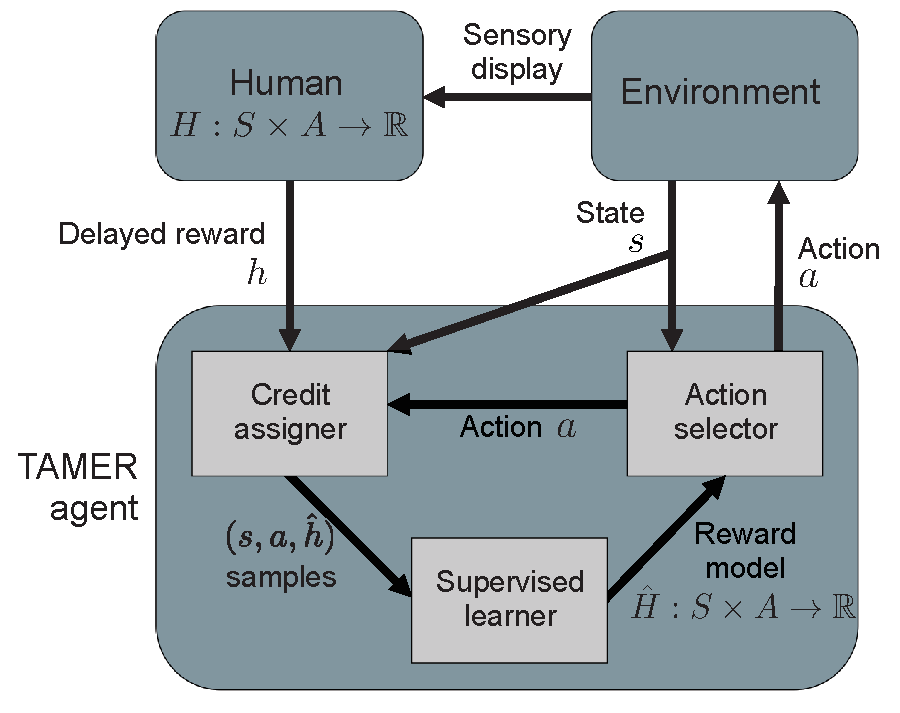
\includegraphics[width=2.8in]{HumanAgentEnvConceptualDiagram}
\caption{Interaction in the TAMER framework (reproduced from \protect\cite{knox2012learning}). }
\label{HumanAgentEnvConceptualDiagram}
\end{figure}


Specifically, it learns a function $\hat{R}_{H}(s, a)$ that approximates the expected human reward conditioned on the current state and action, $R_{H}: S \times A \rightarrow \Re$. Given a state $s$, the agent myopically chooses the action with the largest estimated expected reward, $\argmax_{a}\hat{R}_{H}(s, a)$. The trainer observes the agent's behavior and can give reward corresponding to its quality. The TAMER agent takes each observed reward signal as part of a label for the previous $(s,a)$ and then uses it as a supervised learning sample to update the estimate of $\hat{R}_{H}(s, a)$. %In this paper, the update is performed by incremental gradient descent; i.e., the weights of the function approximator specifying $\hat{R}_{H}(s, a)$ are updated to reduce the error $|r - \hat{R}_{H}(s, a)|$, where $r$ is the sum of reward instances observed shortly after taking action $a$ in state $s$. 


%The TAMER agent strives to maximize the immediate reward, %caused by its action, 
%which contrasts with traditional reinforcement learning, in which the agent seeks the largest discounted sum of future rewards. Until recently, general myopia was a feature of all algorithms involving learning from human feedback and has received empirical support~\cite{knox2015framing}.
%The trainer observes and evaluates the agent's behavior and can give reward. 

The TAMER agent strives to maximize the immediate reward, %caused by its action, 
which contrasts with traditional reinforcement learning, in which the agent seeks the largest discounted sum of future rewards. There are two reasons why an agent can learn to perform tasks from a myopic reward value. Firstly, the human reward can be delivered with small delay, which is the time it takes for a trainer to evaluate the agent's action and deliver her feedback. Secondly, the evaluation provided by a human trainer carries a judgment of the behavior itself with a mental model of its long-term consequences in mind. 
Until recently, general myopia was a feature of all algorithms involving learning from human feedback and has received empirical support~\cite{knox2015framing}.

%The intuition for why an agent {\it can} learn to perform tasks using such a myopic valuation of reward is that human feedback can generally be delivered with small delay---the time it takes for the trainer to assess the agent's behavior and deliver feedback---and the evaluation that creates a trainer's reward signal carries an assessment of the behavior itself, with a model of its long-term consequences in mind. Until recently~\cite{knox2013learning}, general myopia was a feature of all algorithms involving learning from human feedback and has received empirical support~\cite{knoxreinforcement}. Built to solve a variant of a Markov decision processes, (i.e., a specification of a sequential decision-making problem commonly addressed through reinforcement learning \cite{sutton1998reinforcement}) in which there is no reward function encoded before learning, the TAMER agent learns a function $\hat{H}(s, a)$ that approximates the expectation of experienced human reward, $H: S \times A \rightarrow \Re$. Given a state $s$, the agent myopically chooses the action with the largest estimated expected reward, $\argmax_{a}\hat{H}(s, a)$. The trainer observes the agent's behavior and can give reward corresponding to its quality.

%The TAMER agent takes each observed reward signal as part of a label for the previous $(s,a)$ and then used it as a supervised learning sample to update the estimate of $\hat{H}(s, a)$. In this paper, the update is performed by incremental gradient descent; i.e., the weights of the function approximator specifying $\hat{H}(s, a)$ are updated to reduce the error $|r - \hat{H}(s, a)|$, where $r$ is the sum of reward instances observed shortly after taking action $a$ in state $s$.

%In this paper, \HH{Can we claim novelty here? i.e. showing that TAMER can be used to learn a model tree? In reality, we still had to be careful with the types of input features used... however, this was not neccessarily a straight-forward task.}the TAMER agent learns a \emph{model tree} \cite{quinlan1992learning} that constructs a tree-based \HH{this part doesn't make sense to me. Which part of the model is piecewise-linear? the update update of the tree node, parameters? For completeness, I think it would be a good idea to elaborate on the method here in a bit more detail. It's not clear here also why we had to use this method and not the existing TAMER setup. Wouldn't this paragraph be better placed and elaborated upon in the infinit Mario part? } piecewise-linear model to estimate $\hat{R}_{H}(s, a)$.  The TAMER agent takes each observed reward signal as part of a label for the previous $(s,a)$ and then uses it as a supervised learning sample to update the model tree by the divide-and-conquer method.  %In this paper, the TAMER agent learns a update is performed by a model tree \cite{quinlan1992learning}; i.e., the weights of the function approximator specifying $\hat{H}(s, a)$ are updated to reduce the error $|r - \hat{H}(s, a)|$, where $r$ is the sum of reward instances observed shortly after taking action $a$ in state $s$.

In the TAMER framework, the trainer observes and evaluates the agent's behavior and can give reward %. the human trainer provides feedback 
by pressing two buttons on the keyboard, which are assigned to the agent's most recent action. Each press of the two buttons is mapped to a numeric reward of -1 or +1 respectively. The human trainer can strengthen her feedback by pressing either button multiple times and the label for a sample is calculated as a delay-weighted aggregate reward based on the probability that a human reward signal targets a specific time step \cite{knox2012learning}.  %The reward value was always bounded between -4 and +4. %(up to $\pm 4$). 
%The interface flashes blue or red for positive or negative reward, respectively, to inform the trainer when she is giving feedback. 
A TAMER agent learns by repeatedly taking an action, sensing reward, and updating $\hat{R}_{H}$. Note that unlike \cite{knox2012learning}, when no feedback is received from the trainer, learning is suspended until the next feedback instance is received. 

%\vspace{-1mm}
%\HH{I'm not sure if this belongs in the background section... It mixes our implementation in with existing implementations. It undersells the fact that porting Infinite mario into TAMER was not straightforward. I think it might make more sense to put this in a different section as a description of the novel proposed methodology that is used to evaluate our experimental conditions. The clarity and narrative in this part is also confusing. You really need to explain the concepts step by step so it's clear which are the states, which paossible actions there are...currently, new knowledge about the states does not appear all at once but trickles in a bit as a time almost incidentally as you're describing othe parts of the set up. It's really not easy to get a mental picture of what's happening.}


\section{Infinite Mario Domain}
%\vspace{-1mm}
\label{sec:domain}

Super Mario Bros is an extremely popular video game, %and has been ranked first on the ``Top 100 Video Games of All Time''\footnote{\url{http://en.wikipedia.org/wiki/Super\_Mario\_Bros.}}, 
making it an excellent platform for investigating how humans interact with agents that are learning from them. %We used 
To establish the generalizability of TAMER to more complex domains, and to make the experiment appealing to trainers of all ages, we implemented TAMER in the Infinite Mario domain from the Reinforcement Learning Competition \cite{whiteson2010reinforcement,dimitrakakis2014reinforcement} that was adapted from the classic Super Mario Bros video game. %\HH{To establish the generalisability of TAMER to more complex domains, and to make the experiment appealing to trainers of all ages, we implemented}

%Infinite Mario is a complex and challenging domain from the Reinforcement Learning Competition \cite{whiteson2010reinforcement} that was adapted from the classic Super Mario Bros video game. 
The Mario avatar must move towards the right of the screen as fast as possible %to the right as soon as possible 
and at the same time collect as many points as possible. To facilitate comparisons of TAMER with other learning methods that have been applied to this domain, we used the standard scoring mechanism that was established for the Reinforcement Learning Competition, which gives positive reward for killing a monster (+1), grabbling a coin (+1), and finishing the level (+100).  It gives negative points for dying (-10) and for each time step that passes (-0.01). The actions available for Mario %correspond to the buttons on a standard Nintendo controller, which 
are (left, right, no direction), (not jumping, jumping) and (not sprinting, sprinting), resulting in 12 different combined actions for the agent at every time step. The state space is quite complex, as Mario observes a 16 $\times$ 21 matrix of tiles, each of which has 14 possible values. 

To reduce the state space, in our TAMER implementation we consider an 8 $\times$ 8 region of tiles around Mario as his state. The state representation includes properties of Mario and two picked tiles within the 8 $\times$ 8 region ranked by priority of whether it is a pit, monster, block and distance. %\sw{I don't understand this: are you describing the state representation or the actions that are available?} 
%\HH{How is the distance relevant in this case? Isn't it always 1 tile away?} 
%\sw{I still don't understand how the agent can ``search'' the state space.  When does this searching occur?  How does the agent decide where to search? What does it have to do with the state represention?}
For the two selected tiles, the properties include whether it is a pit, monster, mushroom, flower, coin, smashable block or question block and the distance from Mario. The properties of Mario include whether it is at the right of a wall and the speed of it.
%\HH{This gets a bit confusing. You didn't mention mushrooms or flowers before... or whether the block was smashable block, questionmark or coin. Aren't they also part of the state? Or is there a set of possible states for each tile to be in? You describe all this part as if the reader should already know. Given how crucial this part is to the paper and the fact that this is part of the novel implementation, you need to introduce it properly.}
%and the distance from Mario and whether it is a smashable block, a question mark block or a coin. Apart from these, we also select whether Mario is at the right of a wall and the speed of Mario as features of the state representation %\HH{this is quite confusing. You mentioned only pit, monster, block and distance before as the state representation. And now you say that being speed and walls are also part of the state representation. This was not mentioned before!}. 
Thus, the feature vector $\Theta$ for the state representation is 
\begin{equation}
\label{eqn:sr}
 \Theta = [\phi_{1}, \phi_{2}, \phi_{M}],
\end{equation}
where $\phi_{1}$ and $\phi_{2}$ are two vectors for the two selected state features with each consisting of the above properties, and $\phi_{M}$ is a vector consisting of the properties of Mario.

In this paper, %\HH{Can we claim novelty here? i.e. showing that TAMER can be used to learn a model tree? In reality, we still had to be careful with the types of input features used... however, this was not neccessarily a straight-forward task.}
the TAMER agent learns a \emph{model tree} \cite{wang1996induction} that constructs a tree-based %\HH{this part doesn't make sense to me. Which part of the model is piecewise-linear? the update update of the tree node, parameters? For completeness, I think it would be a good idea to elaborate on the method here in a bit more detail. It's not clear here also why we had to use this method and not the existing TAMER setup. Wouldn't this paragraph be better placed and elaborated upon in the infinit Mario part? } 
piecewise-linear model to estimate $\hat{R}_{H}(s, a)$.  
The inputs to $\hat{R}_{H}$ are the above state representation %properties of the two selected tiles, features of Mario, 
and the combined action. %\sw{You mean these are the inputs to $H$?  Make this more precise.}
%The TAMER agent takes each observed reward signal as part of a label for the previous $(s,a)$ and then uses it as a supervised learning sample to update the model tree by the divide-and-conquer method. The model tree can have multivariate linear models at each node with only features tested in the subtree of the current node instead of using all features, analogous to piecewise linear functions. We use model tree because features for state representation are mostly binary and not all features are always relevant. Model tree can select the relevant subset of the features to predict the human reward, thus resulting in more accurate prediction. 

%The inputs to $\hat{R}_{H}$ are the above state representation %properties of the two selected tiles, features of Mario, 
%and the combined action. %\sw{You mean these are the inputs to $H$?  Make this more precise.}
%The TAMER agent takes each observed reward signal as part of a label for the previous $(s,a)$ and then uses it as a supervised learning sample to update the model tree by the divide-and-conquer method.  %In this paper, the TAMER agent learns a update is performed by a model tree \cite{quinlan1992learning}; i.e., the weights of the function approximator specifying $\hat{H}(s, a)$ are updated to reduce the error $|r - \hat{H}(s, a)|$, where $r$ is the sum of reward instances observed shortly after taking action $a$ in state $s$.

In our study, %this version of the game, 
we have 3 levels (0, 1 and 2) with seed 121 %\sw{What does this mean?} 
in Infinite Mario domain. %in our study. 
Level 0 is the same as in the Reinforcement Learning Competition. %and we designed levels 1 and 2. 
We designed level 1 and 2 %were designed 
with increased difficulties, e.g., increasing the number of monsters, changing the type of monsters, adding one pit, changing the height of walls and length of flat stretches, etc. As in Super Mario Bros, Mario can enter the next level automatically if he finishes one level. The game goes back to level 0 if Mario dies or finishes level 2. A given game ends when Mario dies. %\HH{You need to add a decription of how levels 1 and 2 are designed to increase difficulty.}

To see whether a TAMER agent can successfully learn to play the game and compare the learning performance with other methods, one of the authors trained the agent on level 0 with seed 121 %\HH{I dont' recall any prior mention of the difficulty level or seed. If this is important, then you should also mention this in the experimental set up.} 
in the Infinite Mario Domain for 10 trials with TAMER. 
%Figure \ref{setup&feedback&performance}c shows the average offline performance per episode. 
An episode ends when Mario dies or finishes the level. The policy was frozen and recorded at the end of each episode of training. Then, each recorded policy was tested for 20 games offline. The performance for each episode %in Figure \ref{setup&feedback&performance}c 
was averaged over the 20 games and then over the 10 trials. The result shows that our TAMER agent can achieve 120 points in 12 episodes, while it takes about 500 episodes for a SARSA agent to achieve a similar performance level \cite{taylor2011teaching} and a hierarchical SARSA agent implemented with object-oriented representation about 50 episodes to reach a similar level and 300 episodes to achieve 149.48 points \cite{mohan2011object}, which is almost optimal. Although the TAMER agent does not learn an optimal policy, it can successfully learn a good policy substantially faster than these other methods, making this set-up very suitable for our experiments with members of the public where each training session can only last up to 15 minutes.
 %\HH{It's great that you did this. Very good!} 
%\HH{I wonder if this part would be better described in the experimental set up. This part isn't really a result in itself but a way of showing that we did some serious experimental preparation to verify the efficacy of the set up. }

%\vspace{-4mm}\HH{I think you may need to move this before the experimental conditions. I think it would make more sense to explain the physical set up in the room and where the cameras were. I think you also need to explain important information about how they sat in the room. i.e. they could not see the screens of the people and did not sit facing each other.....etc. You also don't mention what they gave consent for. }

\section{Experimental Setup}
%\vspace{-1mm}
\label{sec:es}

%\HH{consider moving this before the conditions as the conditions are limited to some extent by the conditions of the NEMO science live programme.}

Our user study was conducted in conjunction with the research program of the NEMO science museum in Amsterdam.  This program enables museum visitors to participate as experimental subjects in studies conducted by scientists from nearby universities.  In our experiment, a group of up to four trainers, typically a family or group of friends, trained their own TAMER agents at the same time. In each group, each subject sat at her own table, facing away from the other members' and their screens. There was also a camera on the screen in front of the trainer's face. Each participant signed a consent form (with parental consent for children under 18 years old) permitting recording the data and using it for research.
%and was briefed before the experiment about instructions. %\HH{about what?}. 
Then participants in the group were asked to train their own agents for 15 minutes in the same room at the same time. 

Each participant could quit at any time she wanted before the 15 minutes elapsed. Finally, we debriefed the participants and asked for feedback and comments. The experiment was carried out in the local language with English translations available for foreign visitors. We recorded the training data including state observations, actions, human rewards and timestamp, scores, timestamp for each time step, and video data of facial expressions and key presses on the keyboard for each trainer during training. %Trainers were not given time to practice before the experiment because we were concerned that they might get tired of expressing facial emotions after the practice.

%to evaluate the conditions we proposed, as described in Section \ref{sec:cons}. 


%\begin{figure}[htb]
%\vspace{-4mm}
%%\hspace{4mm}
%\centering
%%\begin{tabular}{c c c}
%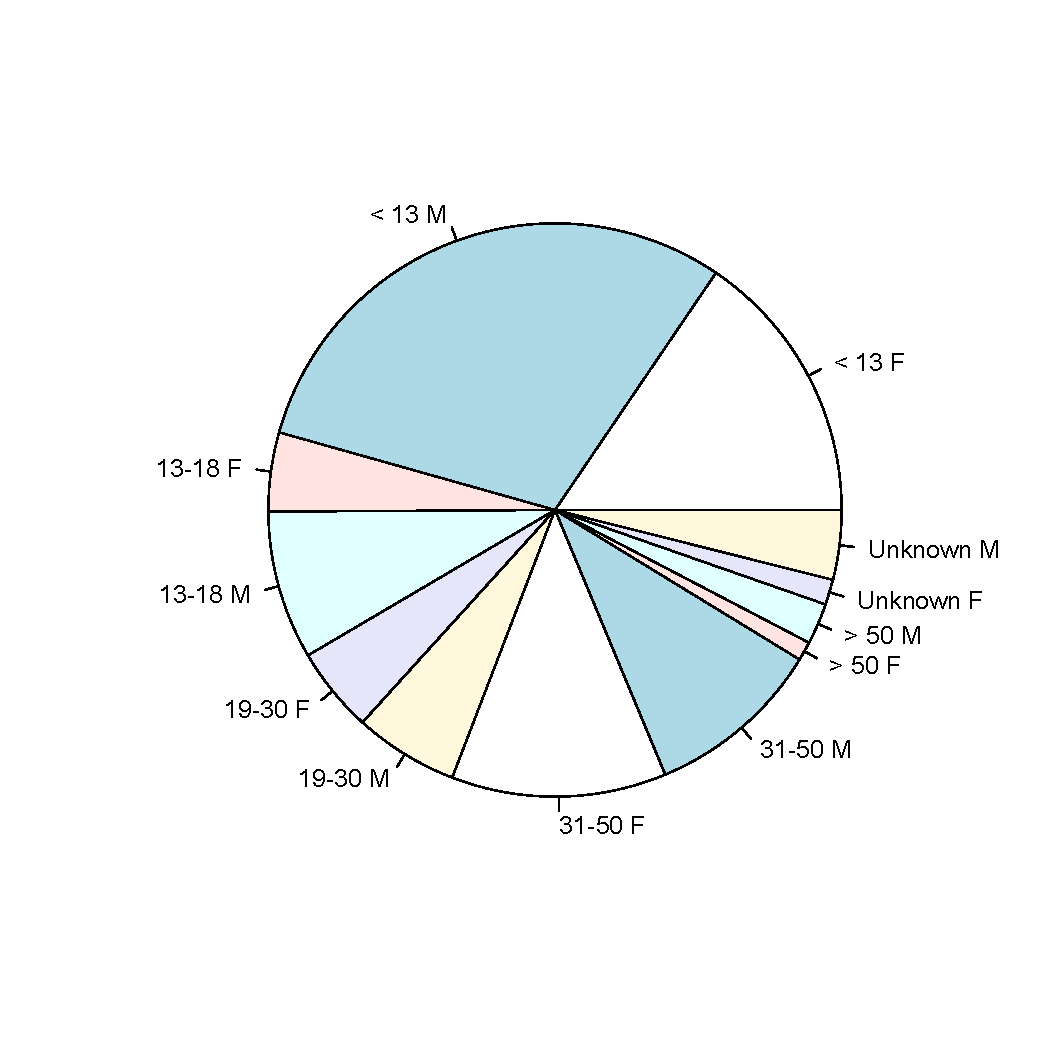
\includegraphics[width=0.7\columnwidth,trim=0 0 0 0, clip]{AgeGenderDistribution}
%%\includegraphics[width=0.4\columnwidth,trim=0 0 0 0, clip]{NumberOfTimeStepsWithFeedback}&
%%\includegraphics[width=0.65\columnwidth,trim=0 0 0 0, clip]{MeanOfflinePerformancePerEpisode} \\
%%a&b&c
%%\end{tabular}
%\vspace{-3mm}
%\caption {Distribution of subjects across age ranges and genders, (F=Female, M=Male).}% b) mean number of time steps with feedback, with and without facial expression and competitiveness and c) mean offline performance per episode trained by one of the authors. Note: black bars in Figure b stand for standard error.}
%\vspace{-4mm}
%\label{demographic}
%\end{figure}

%\HH{I think it is better when describing the actual experimental set up that you do this in the past tense}
Our experiment is a between-subjects study with 561 participants from more than 27 countries participated and %were 
randomly distributed into our four experimental conditions (described below). %i.e., between-subjects study.  %the four conditions described in the next section. %described in previous section. %Section \ref{sec:conditions}. 
Of them, 221 were female and 340 were male respectively, aged from 6 to 72. Figure \ref{demographic} %Figure \ref{demographic} 
shows the distribution of participants across age ranges and genders. %As shown in Figure \ref{setup&feedback&performance}a, %\HH{please do make sure that both gender distributions for different age categories are shown}, %256 (87 females and 169 males) subjects younger than 13 years old, 72 (25 females and 47 males) subjects between 13 and 18 years old, 60 (27 females and 33 males) subjects between 19 and 30 years old, 124 (68 females and 56 males) subjects between 31 and 50 years old, 19 (6 females and 13 males) subjects older than 50 years old and 30 (8 females and 22 males) 
%45.6\% of the subjects were less than 13 years old, 13\% were between 13 and 18 years old, 10.7\%  were between 19 and 30 years old, 22\% were between 31 and 50 years old, 3.4\% were more than 50 years old and  5.3\% subjects did not report their age.
%\footnote{Some subjects did not fill in the age or fill the wrong age in the consent form.} %\HH{Please give distribution across the age ranges and gender as text and also as bar graphs. You have space - the graphs in the paper currently are quite big...when you shrink the figures, you will also need to increase the font size. It is currently far too small.}. 
Data from 63 participants were disregarded: five participants lacked parental consent; three had not played Super Mario Bros before and were unable to judge Mario's behavior; one had an internet connection problem, one quit after only five minutes' training; and the rest did not fully understand the instructions, got stuck and gave feedback randomly by alternating positive and negative feedback in quick succession, or interrupted their family members. %because they did not understand the instructions and gave feedback randomly by pressing the buttons in turn. The choice was made based on the judgment of the experimenter during the experiment and by checking the recorded audio, video, and key presses afterwards. \sw{This still seems really vague to me.} %\HH{You need to elaborate on how this choice was made to show that the selection of these bad data points was performed as objectively as possible.} 
After pruning the data, 498 participants remained: 109 participants in the control condition; 100 in the facial expression condition; 135 in the competitive condition; and 154 in the competitive facial expression condition.

\begin{figure}[tb]
%\vspace{-2mm}
%\hspace{4mm}
\centering
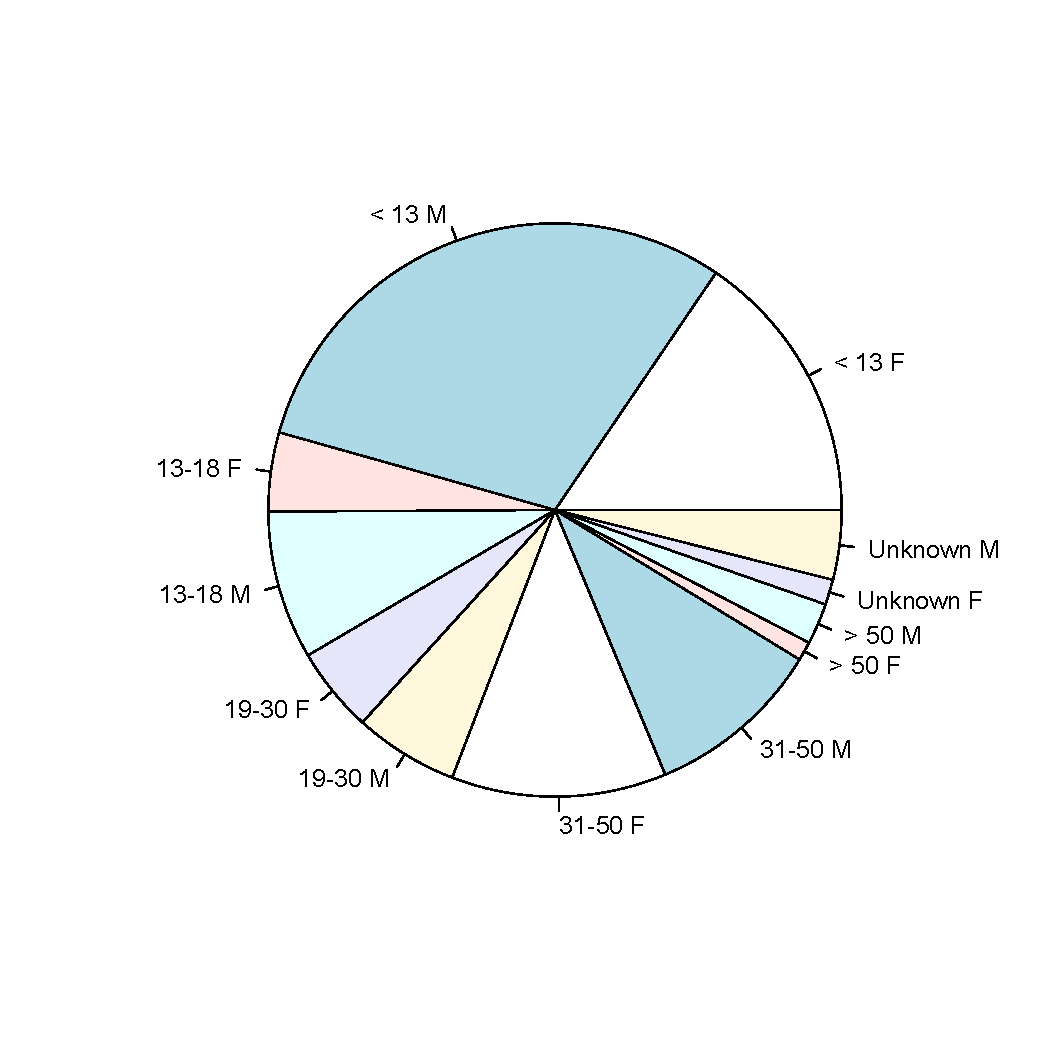
\includegraphics[width=0.9\columnwidth,trim=10 10 10 0, clip]{AgeGenderDistribution} 
%\vspace{-15mm}
\caption{ Demographic information of participants across age ranges and genders in our study. (F=Female, M=Male)}%\HH{Can you also include the gender in the pie chart (this is what I had meant before...?) }}%\sw{``Feedback'' should be lowercase in the graph header.}}
%\vspace{-4mm}
\label{demographic}
\end{figure}

%\begin{table}[htb]
%%\vspace{-2mm}
%\centering
%%\caption{Demographic information of participants in our experiment. }%Distribution of subjects across age ranges and genders.}
%\vspace{2mm}
%\begin{tabular}{ | r | c | c | c |}
%\toprule
%& Under 13 & 13 to 30 & Above 30  \\
%\toprule
%\textbf{Female} & 90 & 57 &74\\
%\hline
%\textbf{Male} & 187 & 81 & 72 \\
%\toprule
%\end{tabular}
%\caption{Demographic information of participants in our experiment. }
%%\vspace{-4mm}
%\label{demographic}
%\end{table}

%\vspace{-1mm}
\section{Experimental Conditions}
%\vspace{-1mm}
\label{sec:cons}

%In this section, we propose two variations on the baseline TAMER interface described above that each display additional information about the agent?s performance history or internal processes. These variations are motivated by the notion that the interaction between the trainer and the agent should be consciously designed to be bidirectional, where the agent gives the trainer informative and/or motivating feedback about its learning process. Our intuition is that such feedback will help keep the trainer?s involvement in the training process and empowers them to offer more useful feedback. More objectively, we hypothesize that doing so will increase the quantity of the trainer?s feedback and improve the agent?s task performance.

In this section, we describe the four conditions we proposed and tested in our experiment. We investigate how the agent's competitive feedback---the agent's performance relative to agents trained by other trainers, and telling trainers to use facial expression as an additional channel to train agents affect %the amount of feedback received by the agent, 
the agent's learning performance and trainer's facial expressiveness. We hypothesize that the agent's competitive feedback will motivate the trainer to train agents better, and telling to use facial expression will %reduce the number of keypress feedback received from the trainer and 
result in worse agent performance as it might distract the trainer from giving high quality keypress feedback. In addition, we expect that both the agent's competitive feedback and telling to use facial expression will increase the trainer's facial expressiveness.

%The interfaces for the control and trick facial expression conditions are replicated from \cite{li2013using}. 
Note that as in the original TAMER, %participants in all four conditions could give positive and negative feedback by pressing buttons on the keyboard to reward or punish the previous action of the agent. Their feedback can be strengthened by pressing the button multiple times. The reward value was always bounded between -4 and +4. 
in all conditions, participants could give positive and negative feedback by pressing buttons on the keyboard to train the agent. Only the key press signal was used for agent learning and videos of training by participants in all conditions were recorded. 

%\vspace{-1mm}
\subsection{Control Condition} 
%\vspace{-1mm}
The interface for the control condition is the performance-informative interface replicated from \cite{li2015using} and implemented in the Infinite %\HH{ Can you just write the name of the game in full?i.e. Super Mario Brothers}
Mario domain, as shown in Figure \ref{control}. %Apart from the state and action of the agent, which are visible from the game board, the agent's performance over past and current games is shown in a performance window during the training process. The performance window allows the agent to give the trainer %\HH{I would suggest to remove 'motivating'. This is more speculatory than proven...} %motivating 
%feedback about its learning process and keeps the trainer involved in the training process \cite{li2013using}. Trainers in this condition were told to use key presses to train the agent.

%\HH{You must say that video was recorded of the trainer while they trained the agent and that they were informed of this fact. Depending on the ordering of the sections (as I have suggested in the earlier comment), you can either put it here, or in the experimental set up. However, it's important for the experimental design that they knew that they were being recorded with video and that their parents were also aware of this fact wrt. their children. }
%and empowers her to give useful feedback. %\sw{Why?} 

%\begin{figure}[htb]
%\centering
%\begin{tabular}{c c}
%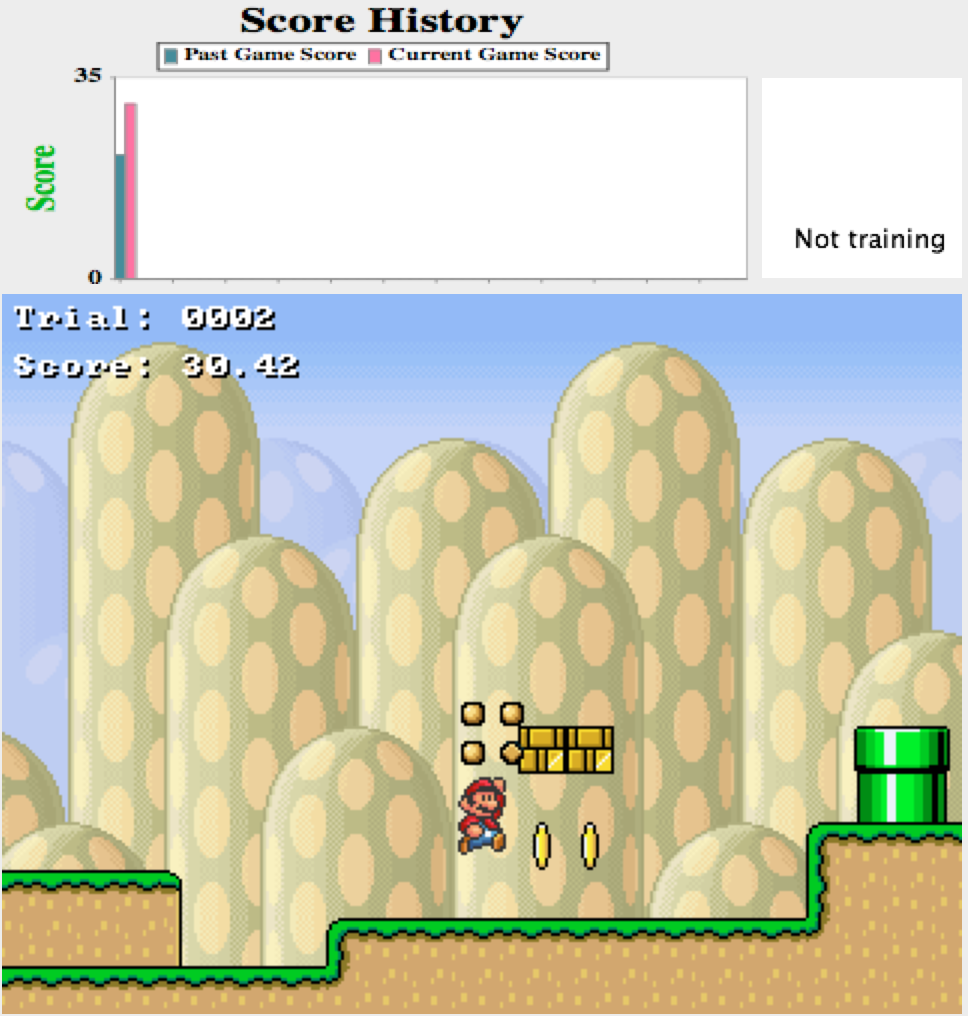
\includegraphics[width=0.5\linewidth]{control} & 
%\includegraphics[width=0.4\columnwidth,height=1.7in]{NumberOfTimeStepsWithFeedbackScoreLevel.pdf}\\
%(a)&(b)
%\end{tabular}
%%\vspace{-4mm}
%\caption{(a) The training interface in the control condition, (b) mean number of time steps with feedback received by agents in level 0, 1 and 2 in the game. Note: error bars represent standard error.}
%%\vspace{-5mm}
%\label{control&feedback}
%\end{figure}

\begin{figure}[htb]
\centering
%\begin{tabular}{c c}
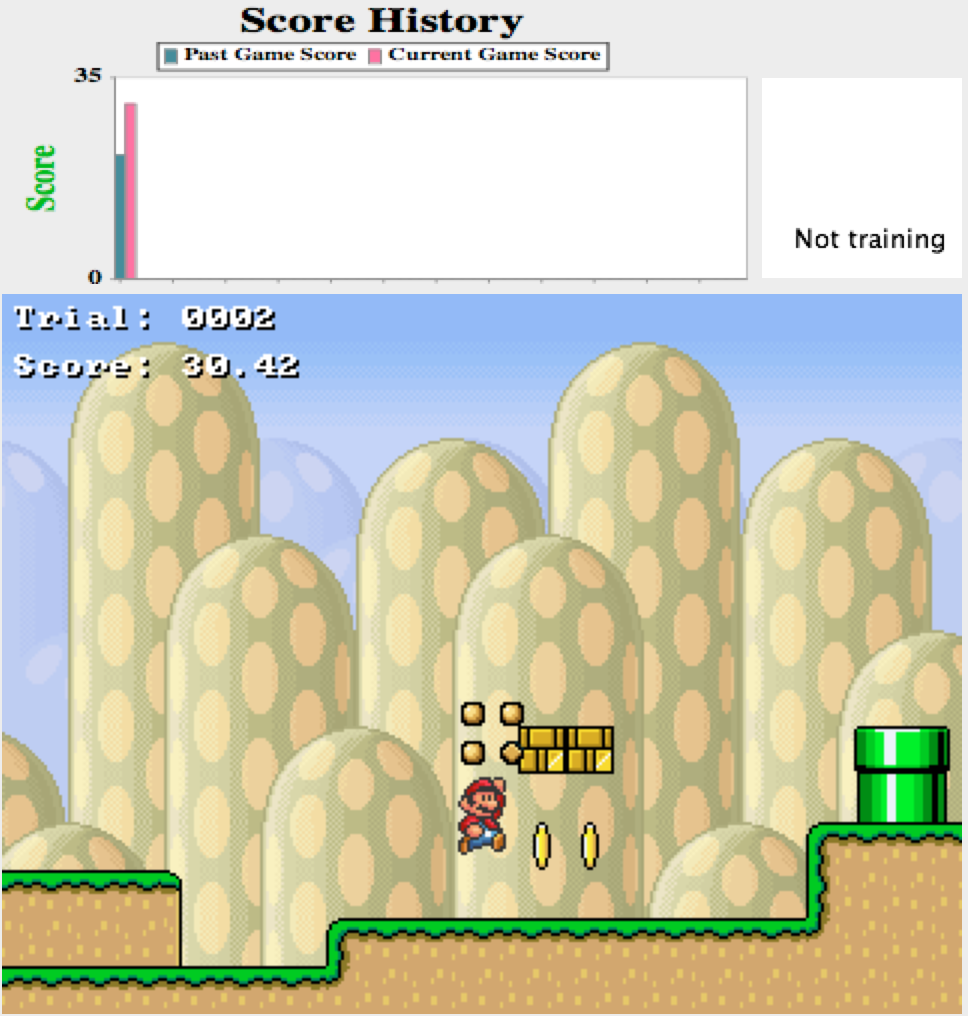
\includegraphics[width=0.75\linewidth]{control} %& 
%\includegraphics[width=0.4\columnwidth,height=1.7in]{NumberOfTimeStepsWithFeedbackScoreLevel.pdf}\\
%(a)&(b)
%\end{tabular}
%\vspace{-4mm}
\caption{The training interface used in the control condition. }%(b) mean number of time steps with feedback received by agents in level 0, 1 and 2 in the game. Note: error bars represent standard error.}
%\vspace{-5mm}
\label{control}
\end{figure}

%\begin{figure*}[htb]
%%\vspace{-2mm}
%%\hspace{4mm}
%\centering
%\begin{tabular}{c c c}
%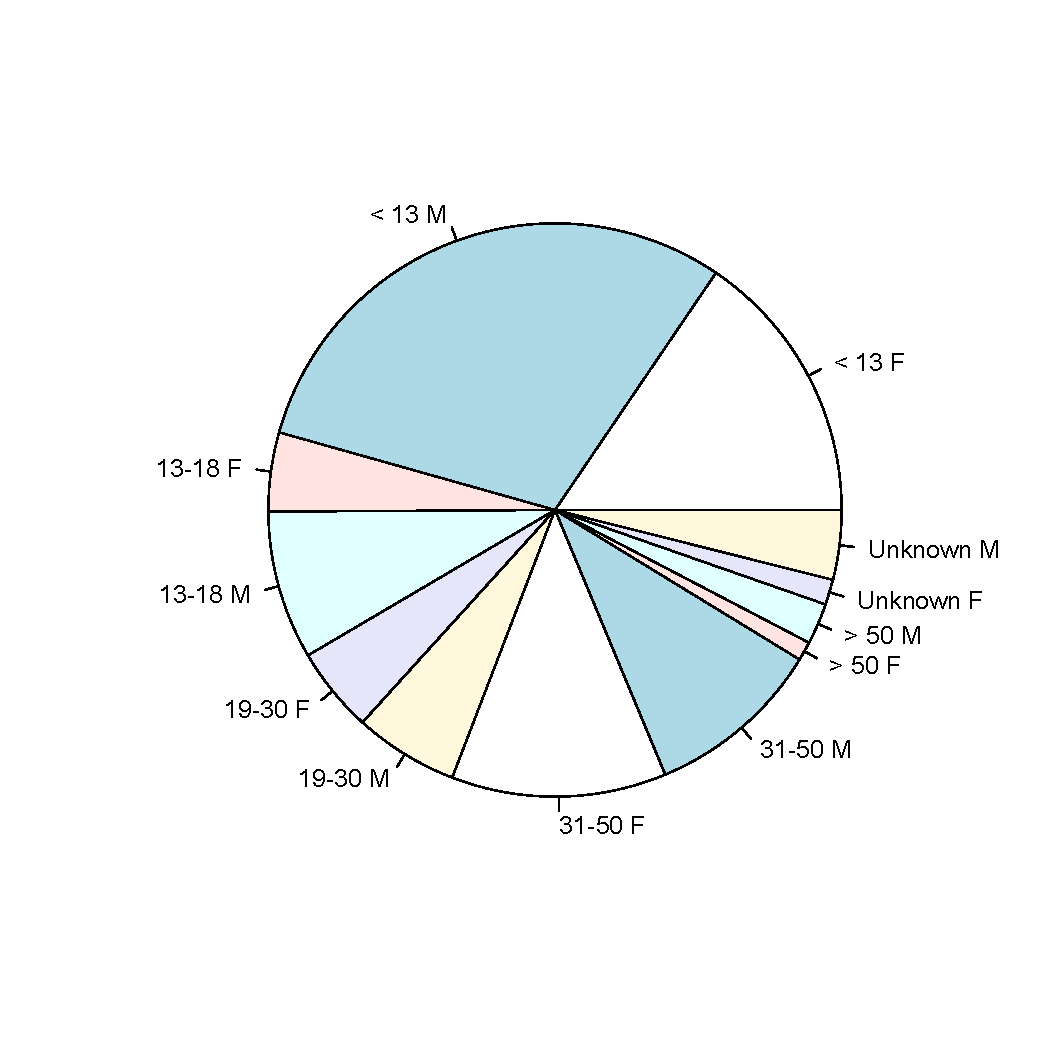
\includegraphics[width=0.7\columnwidth,trim=0 0 0 0, clip]{AgeGenderDistribution}&
%\includegraphics[width=0.4\columnwidth,trim=0 0 0 0, clip]{NumberOfTimeStepsWithFeedback}&
%\includegraphics[width=0.65\columnwidth,trim=0 0 0 0, clip]{MeanOfflinePerformancePerEpisode} \\
%a&b&c
%\end{tabular}
%\vspace{-3mm}
%\caption{ a) Distribution of subjects across age ranges and genders, (F=Female, M=Male), b) mean number of time steps with feedback, with and without facial expression and competitiveness and c) mean offline performance per episode trained by one of the authors. Note: black bars in Figure b stand for standard error.}
%\vspace{-6mm}
%\label{setup&feedback&performance}
%\end{figure*}

%As shown in Figure \ref{control}, 
In the interface, each bar in the performance window above the game board indicates the agent's performance in one game chronologically from left to right. The agent's performance is the score achieved by the Mario agent in the game task. During training, the pink bar represents the score received so far for the current game, while the dark blue bars represent the performance of past games. When a game ends (i.e., Mario dies), the corresponding bar becomes dark blue and a new score received in the new game is visualized by a pink bar to its right. When the performance window is full, the window is cleared and new bars appear from the left. Trainers in this condition were told to use key presses to train the agent.
%Participants could give positive and negative feedback by pressing buttons on the keyboard to reward or punish the previous action of the agent. Their feedback can be strengthened by pressing the button multiple times. The reward value was always bounded between -4 and +4. \sw{Move this to the beginning of Section 5?}

 %\HH{The reward value was always bounded between -4 and +4.}

%\subsection{\HH{We need a new name for this that doesn't sound so vindictive...}Trick Facial Expression Condition}

%\vspace{-1mm}
\subsection{Facial Expression Condition}
%\vspace{-1mm}
The interface used in this condition is the same as in the control condition except that trainers were told to use both key presses and facial expressions to train the agent. We told them this because we wanted to investigate whether telling trainers to use facial expressions as a separate channel to train the agent would affect the trainer's training and agent's learning, compared to trainers in the control condition. We hypothesize that telling trainers to use facial expressions to train the agent will result in worse performing agents than agents trained by those being told to use only key-press feedback to train agents. This is because telling participants to use facial expressions as separate reward signal could induce higher cognitive load thus distracting them from giving high quality key press feedback. In addition, we hypothesize that because of more posed facial behaviors by trainers in this condition, the expressiveness of trainers' facial expression will be higher than those in the control condition. %\sw{Why?} %We hypothesized that the facial behaviour would be more posed and less spontaneous and could be more tiring to give in this condition.

%The interface used in this condition is the same as in control condition. The only difference is that trainers in this condition were told to use both key presses and facial expressions to train the agent. We told them this because we wanted to investigate whether trainers would behave differently, e.g., by exaggerating their facial expressions, if they were told that they have a separate channel to use facial expression to train the agent, compared to trainers in the control condition. We hypothised that the facial behaviour would be more posed and less spontaneous and could be more tiring to give in this condition. %\HH{We hypothesise that the facial behaviour will be more posed and less spontaneous and could be more tiring to give.} 
%Additionally, we hypothesize that compared to trainers in the control condition, the agents trained in facial expression condition will perform worse because less key press feedback is given to train the agents while more desperate facial expressions were performed by trainers. \HH{This second hypothesis is an obvious one. We need to make sure that the hypotheses actually contribute to some interesting and perhaps surprising findings rather than just very obvious and boring things.}

%\vspace{-1mm}

\begin{figure}[htb]
\centering
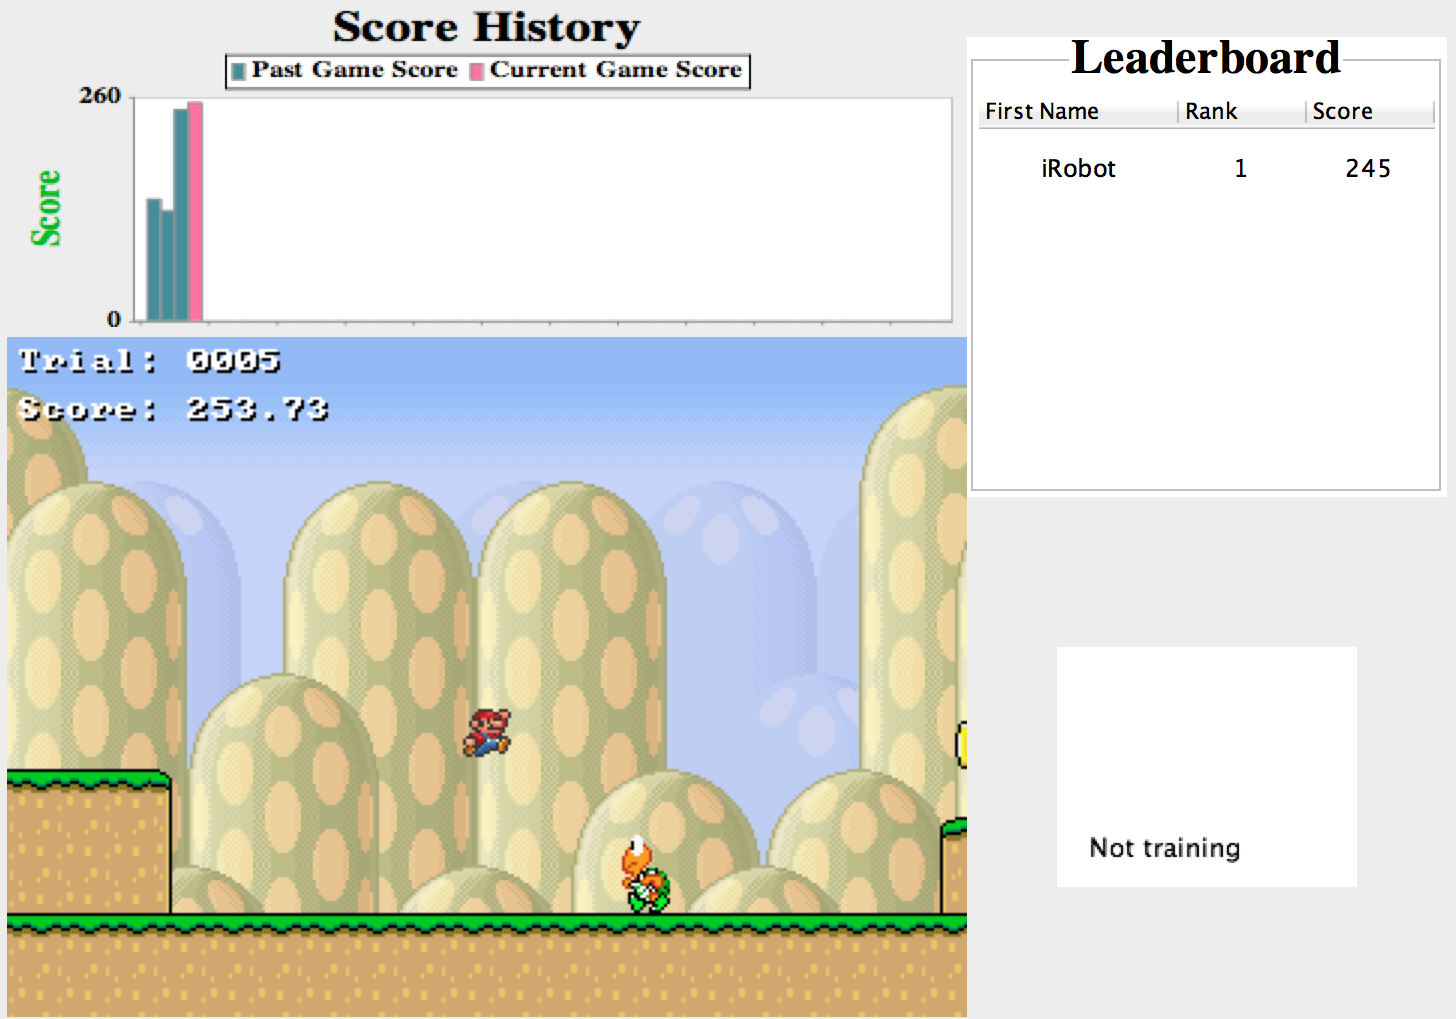
\includegraphics[width=0.85\linewidth]{leaderboard}
%\vspace{-2mm}
\caption{The training interface for the competitive condition.}
%\vspace{-4mm}
\label{leaderboard}
\end{figure}


\subsection{Competitive Condition}%Close-competitive Condition}

In the interfaces used in the control and facial expression conditions, only the agent's own performance was shown to the human trainer. Li et al.\ \cite{li2014learning} showed that putting people in a socio-competitive situation could further motivate them to give more feedback and improve the agent's performance. In this study, we aim to verify this result as well as investigate how it plays out when the socio-competitive setting involves people who know each other and are training at the same time in the same room. In addition, we hypothesize that the expressiveness of trainers' facial expressions in the competitive condition would increase as a result of the agent's competitive feedback compared to those in the control condition. %and the effect of competition on trainers' facial expressions. %We hypothesize that people will be further motivated to improve the agent's performance if they are put in a competitive situation where they can compare the performance of their agents with that of others, especially those closely related people. \sw{This sounds like it's a new idea.  We need to say that a previous study showed that this works and that we wanted to verify it and see how it plays out when people who know each other are training at the same time in the same room.}
Therefore, in the competitive condition, we allow the agent to indicate the rank and score of the other members of the group, who are all training their own agents simultaneously in the same room, as described in the experimental setup in the previous section. The groups typically consist of family members or close friends, e.g., children and (grand) parents, %or grandparents
 brothers and sisters. %\HH{it would be better to actually provide numerical statistics here rather than broad statements - we should at least have the relationship between the adult and the child that they are signing on behalf of.}. 

%We hypothesize that the trainers in the competitive condition will express more and %\HH{You need to express this in more measurable terms.. . I recall you meant 'extreme' facial expressions...this is an interesting one that we could have added to the discussion with Hamdi this afternoon!} 
%extreme facial emotions %and give more key press feedback 
%than those in the control condition. % and the trained agents will perform better finally. 

%This condition is called close-competitive not only because the trainers are closely related, but also they sit and train their own agents in the same location at the same time. %unlike experiment in \cite{li2014leveraging, li2014learning} where trainers compete with each other remotely on the internet and most probably trained their agent at different times 
%\HH{is the submission anonymous? If so, we have to be careful not to draw attention to ourselves as authors of the previous work.}.
%


To implement this condition, we added a leaderboard to the right of the interface used in the control and facial expression conditions, as shown in Figure \ref{leaderboard}. 
In the leaderboard, the first names, scores and ranks of all the group members currently training the agent are shown. When the trainer starts training for the first time, her agent's performance is initialized to 0 and ranked in the leaderboard. Whenever the trainer finishes a game (i.e. Mario dies), the new game score and rank is updated in the leaderboard. To create more movement up and down in the leaderboard, the last game score is always used. The trainer can directly check her score and rank in the leaderboard. Therefore, the trainer can keep track of both the agent's learning progress and the agent's performance relative to that of other members of her group.


%\vspace{-1mm}
\subsection{Competitive Facial Expression Condition}%Trick Facial Expression and Close-compe-titive Condition}
%\HH{I'm not sure whether to use the word 'close'... it implies that there should be another condition where strangers compete with each other. However, we did not have a setup for this... so perhaps socio-competitive in some sense, is more accurate. Also, I think you need to explain why the members of groups were close - it's actually more related to how NEMO was set up.}
The final condition is a combination of the facial expression and competitive conditions. Specifically, the interface is the same as in the competitive condition but, as in the facial expression condition, trainers were told to use both key presses and facial expressions to train agents.  As in other conditions, only key presses were actually used for agent learning. We hypothesize that the expressiveness of trainers' facial expressions in this condition will be much higher than those in the facial expression condition and competitive condition, since trainers in this condition were both told to use facial expressions as additional channel to train the agent and informed competitive feedback by the agent.

%With this condition, we aim to investigate how trainers behave if they are told to use facial expressions to train the agent in a %\HH{close?} socio-competitive 
%competitive situation and whether trainers in this condition behave and train the agent differently from those in the facial expression and competitive conditions. We hypothesize that agents trained in this condition will ultimately perform worse %and receive less key press feedback 
%%and trainers will make more %\HH{extreme} desperate
%%extreme facial expressions 
%compared to those in the competitive condition. Furthermore, we hypothesize that, compared with agents trained in the facial expression condition, agents trained in this condition will perform better finally and receive more key press feedback.% and trainers will make more \sw{Why?} extreme facial expressions. 


%\vspace{-1mm}
\section{Results and Discussion}
%\vspace{-1mm}
\label{sec:re}

In this section, we present and analyze our experimental results. Given the large sample size and game design, since participants in our study span a wide range of ages and two genders, we consider three additional individual variables: age, gender and level, in addition to `competition' and `facial expression' the two tested independent variables. %Here `facial expression' means whether telling trainers to use facial expressions to train agents or not, %as in the facial expression condition and competitive facial expression condition, 
%while `competition' means whether a leaderboard was shown in the training interface. % as in the competitive condition and competitive facial expression condition. 
`Gender' and `age' mean all trainers were divided into females and males and three age groups: under 13, 13 to 30 and older than 30. %, which is also a measure of variance by telling what proportion of the variance in the dependent variable is attributable to the factor in question.
`Level' means the most frequent highest level in the game reached by the agent tested offline: level 0, level 1 and level 2 in the game design.
In the results below, the $p$-values were computed with $n$-way ANOVA ($n$ is the number of factors) since we need to take multiple factors into account, unless indicated otherwise. ANOVA is a test for statistical significance between means by actually comparing the variance due to the between-groups variability with the within-group variability. %for each factor. %\HH{comparing variance between what? The variance of what? You need to be more precise here.}.  \HH{this sentence doesn't really explain anything... it's like saying 'g' is usually used for testing the state. What is eta and how is the calculated? where is 'n'? }
$\eta_{p}^{2}$ is the effect size which indicates %the proportion of variance in the dependent variable explained by the independent variable. 
the variance accounted for by a factor effect and that effect plus its associated error variance within an ANOVA study. Note that the suggested norms for $\eta_{p}^{2}$ are: small = 0.01; medium = 0.06; large = 0.14.  %\cite{cohen2013statistical}. 
%Apart from `competition' and `facial expression' two independent variables, we consider three additional individual variables: %$n=5$ factors: facial expression, competition, 
%age, gender and level. %Here `facial expression' means whether telling trainers to use facial expressions to train agents or not, %as in the facial expression condition and competitive facial expression condition, 
%%while `competition' means whether a leaderboard was shown in the training interface. % as in the competitive condition and competitive facial expression condition. 
%`Gender' and `age' mean all trainers were divided into females and males and three age groups: under 13, 13 to 30 and older than 30. %, which is also a measure of variance by telling what proportion of the variance in the dependent variable is attributable to the factor in question.
%`Level' means the most frequent highest level in the game reached by the agent tested offline.

%\HH{you mention the inclusion of a mode anova later but don't mention it here.... that's pretty confusing...}
%\sw{It's important that the figures be readable in black and white, but it's also nice if they are in color for people who print on a color printer or read the pdf on a computer.}

%\vspace{-3mm}
%\paragraph{Feedback Given}
%\subsection{Feedback Given}
%%\vspace{-1mm}
%
%\begin{wrapfigure}{r}{0.5\columnwidth}
%\vspace{-8mm}
%\begin{center}
%\includegraphics[width=0.45\columnwidth]{NumberOfTimeStepsWithFeedbackScoreLevel.pdf}
%\vspace{-4mm}
%\caption{Mean number of time steps with feedback received by agents in level 0, 1 and 2 in the game. Note: error bars represent standard error.} %with and without facial expression and competitiveness.}
%\label{feedback}
%\end{center}
%\vspace{-4mm}
%\end{wrapfigure}

%\begin{figure}{r}
%\vspace{-8mm}
%\begin{center}
%\includegraphics[width=0.7\columnwidth]{NumberOfTimeStepsWithFeedbackScoreLevel}
%%\vspace{-10mm}
%\caption{Mean number of time steps with feedback for score level 0, 1 and 2.} %with and without facial expression and competitiveness.}
%\label{feedback}
%\end{center}
%%\vspace{-8mm}
%\end{figure}

%\begin{figure}
%\centering
%\includegraphics[width=0.45\columnwidth]{NumberOfTimeStepsWithFeedback}
%\vspace{-6mm}
%\caption{Mean number of time steps with feedback, with and without facial expression and competitiveness.}
%\vspace{-4mm}
%\label{feedback}
%\end{figure}

%\begin{figure}[htb]
%\centering
%%\begin{tabular}{c c}
%%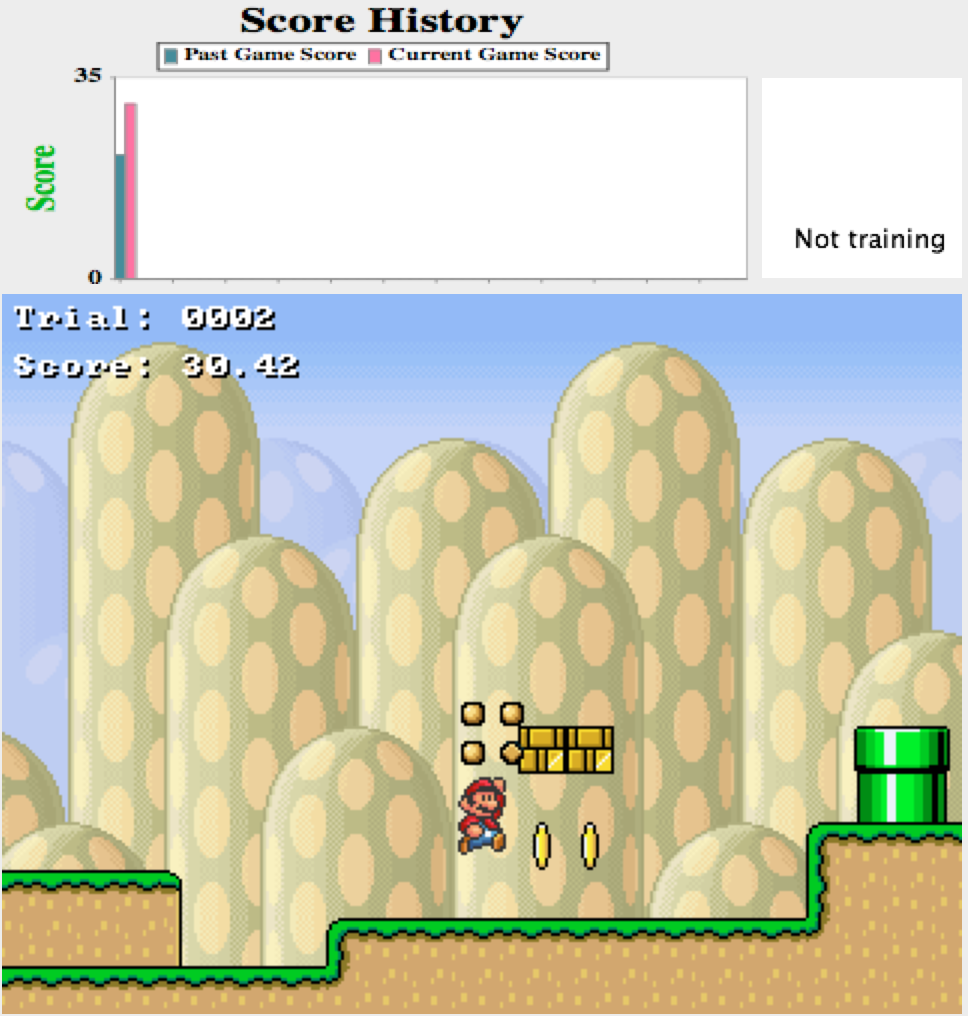
\includegraphics[width=0.5\linewidth]{control} & 
%\includegraphics[width=0.4\columnwidth,height=1.7in]{NumberOfTimeStepsWithFeedbackScoreLevel.pdf}%\\
%%(a)&(b)
%%\end{tabular}
%%\vspace{-4mm}
%\caption{Mean number of time steps with feedback received by agents in level 0, 1 and 2 in the game. Note: error bars represent standard error.}
%%\vspace{-5mm}
%\label{feedback}
%\end{figure}

\begin{figure}
\centering
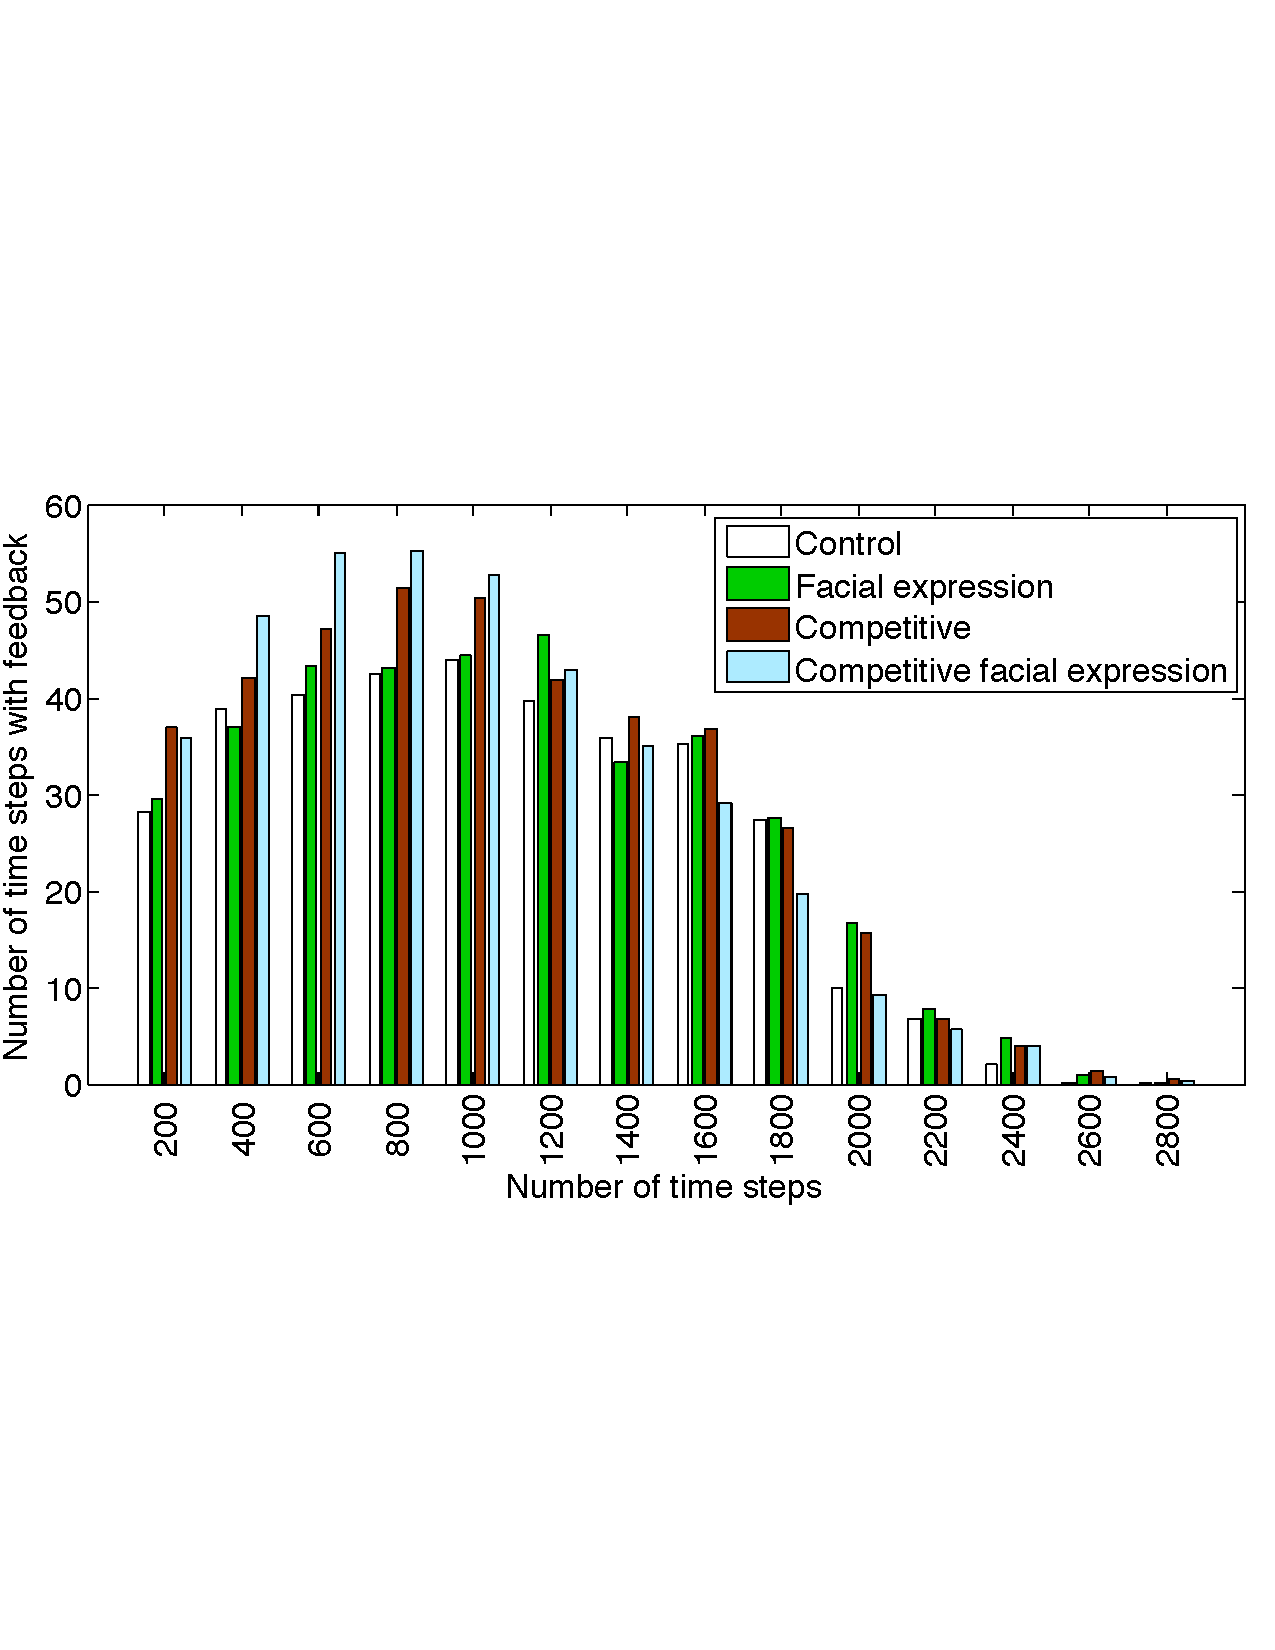
\includegraphics[width=1\columnwidth, height=2.2in,]{FeedbackFrequency}
%\vspace{-6mm}
\caption{Mean number of time steps with feedback per 200 time steps for all four conditions during the training process.}
%\vspace{-4mm}
\label{feedback}
\end{figure}

\begin{figure*}[htb]
%\vspace{-2mm}
%\hspace{-6mm}
\centering
\begin{tabular}{c c c c}
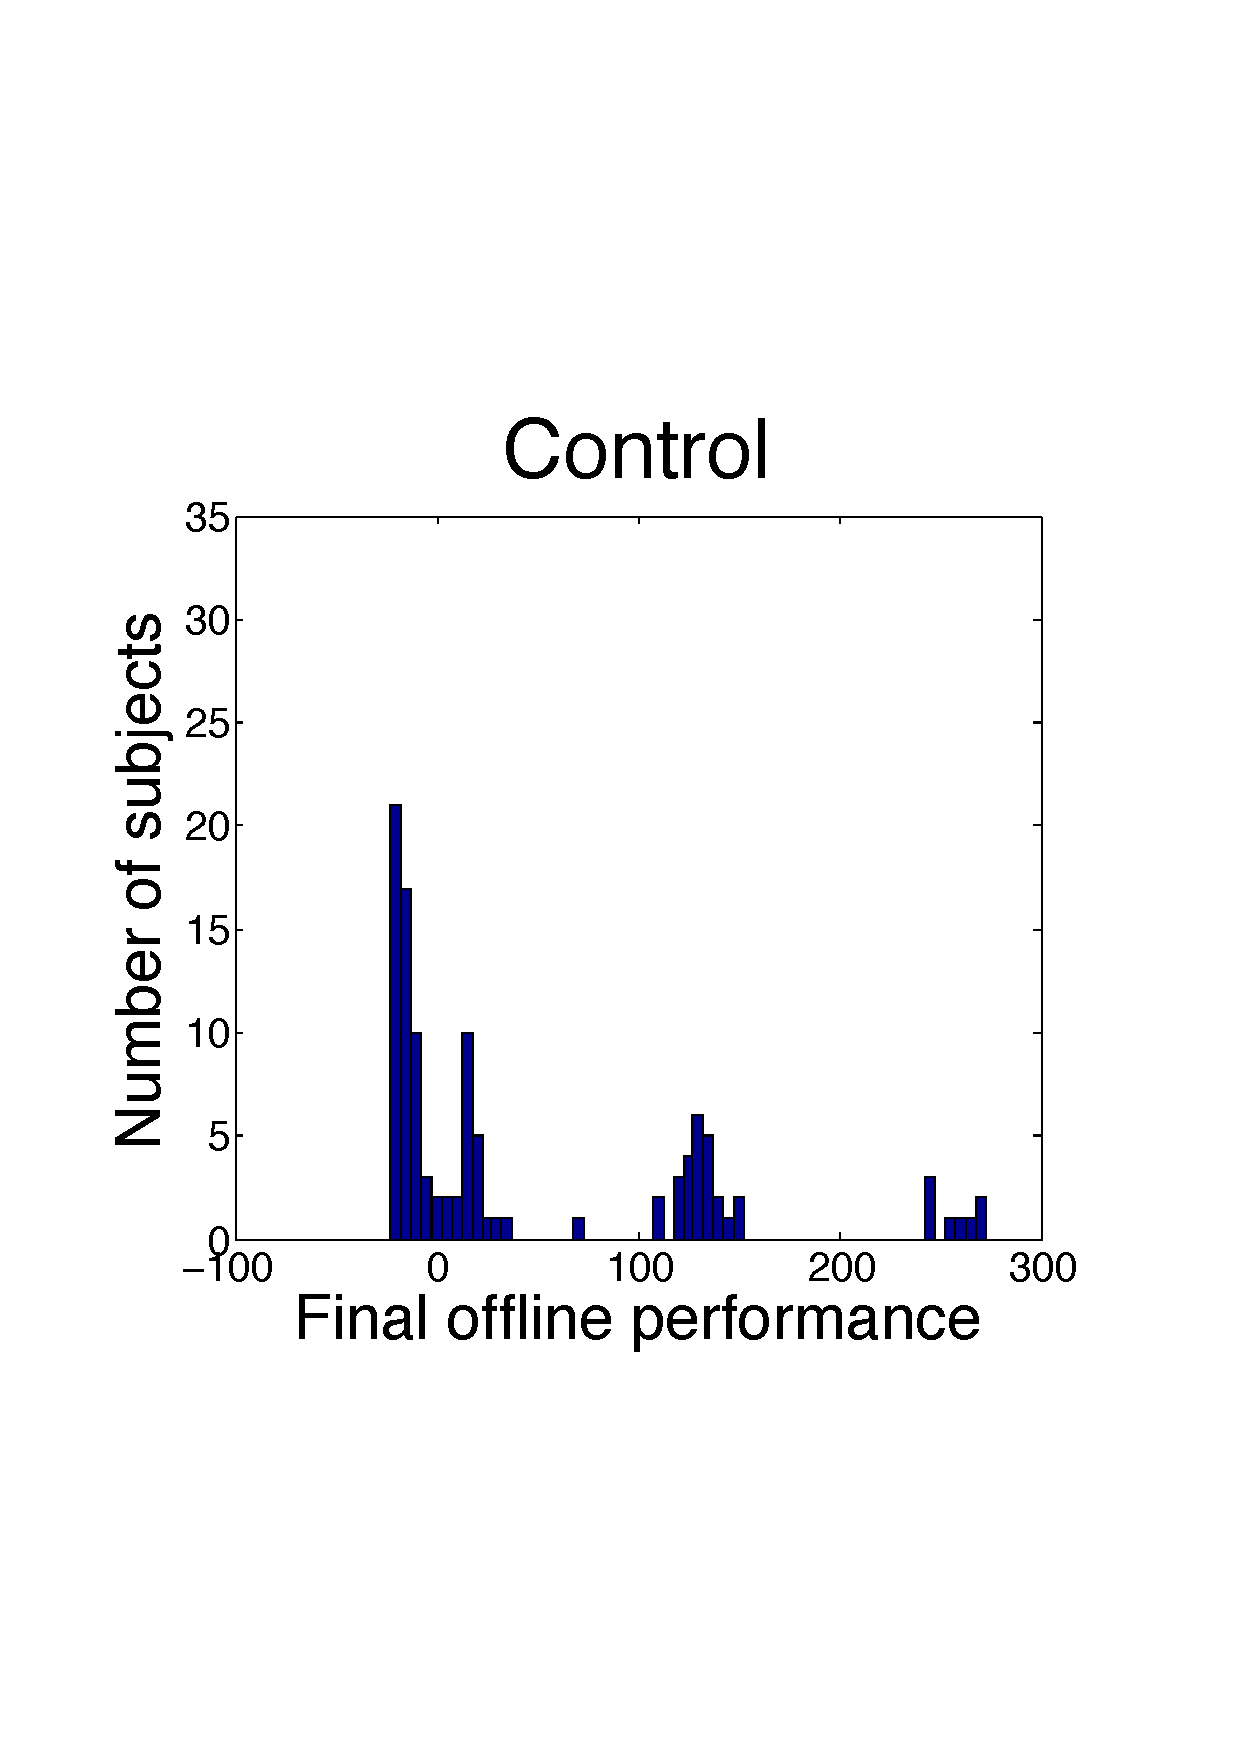
\includegraphics[width=0.47\columnwidth]{DistributionFinalOfflinePerformControl.pdf}&
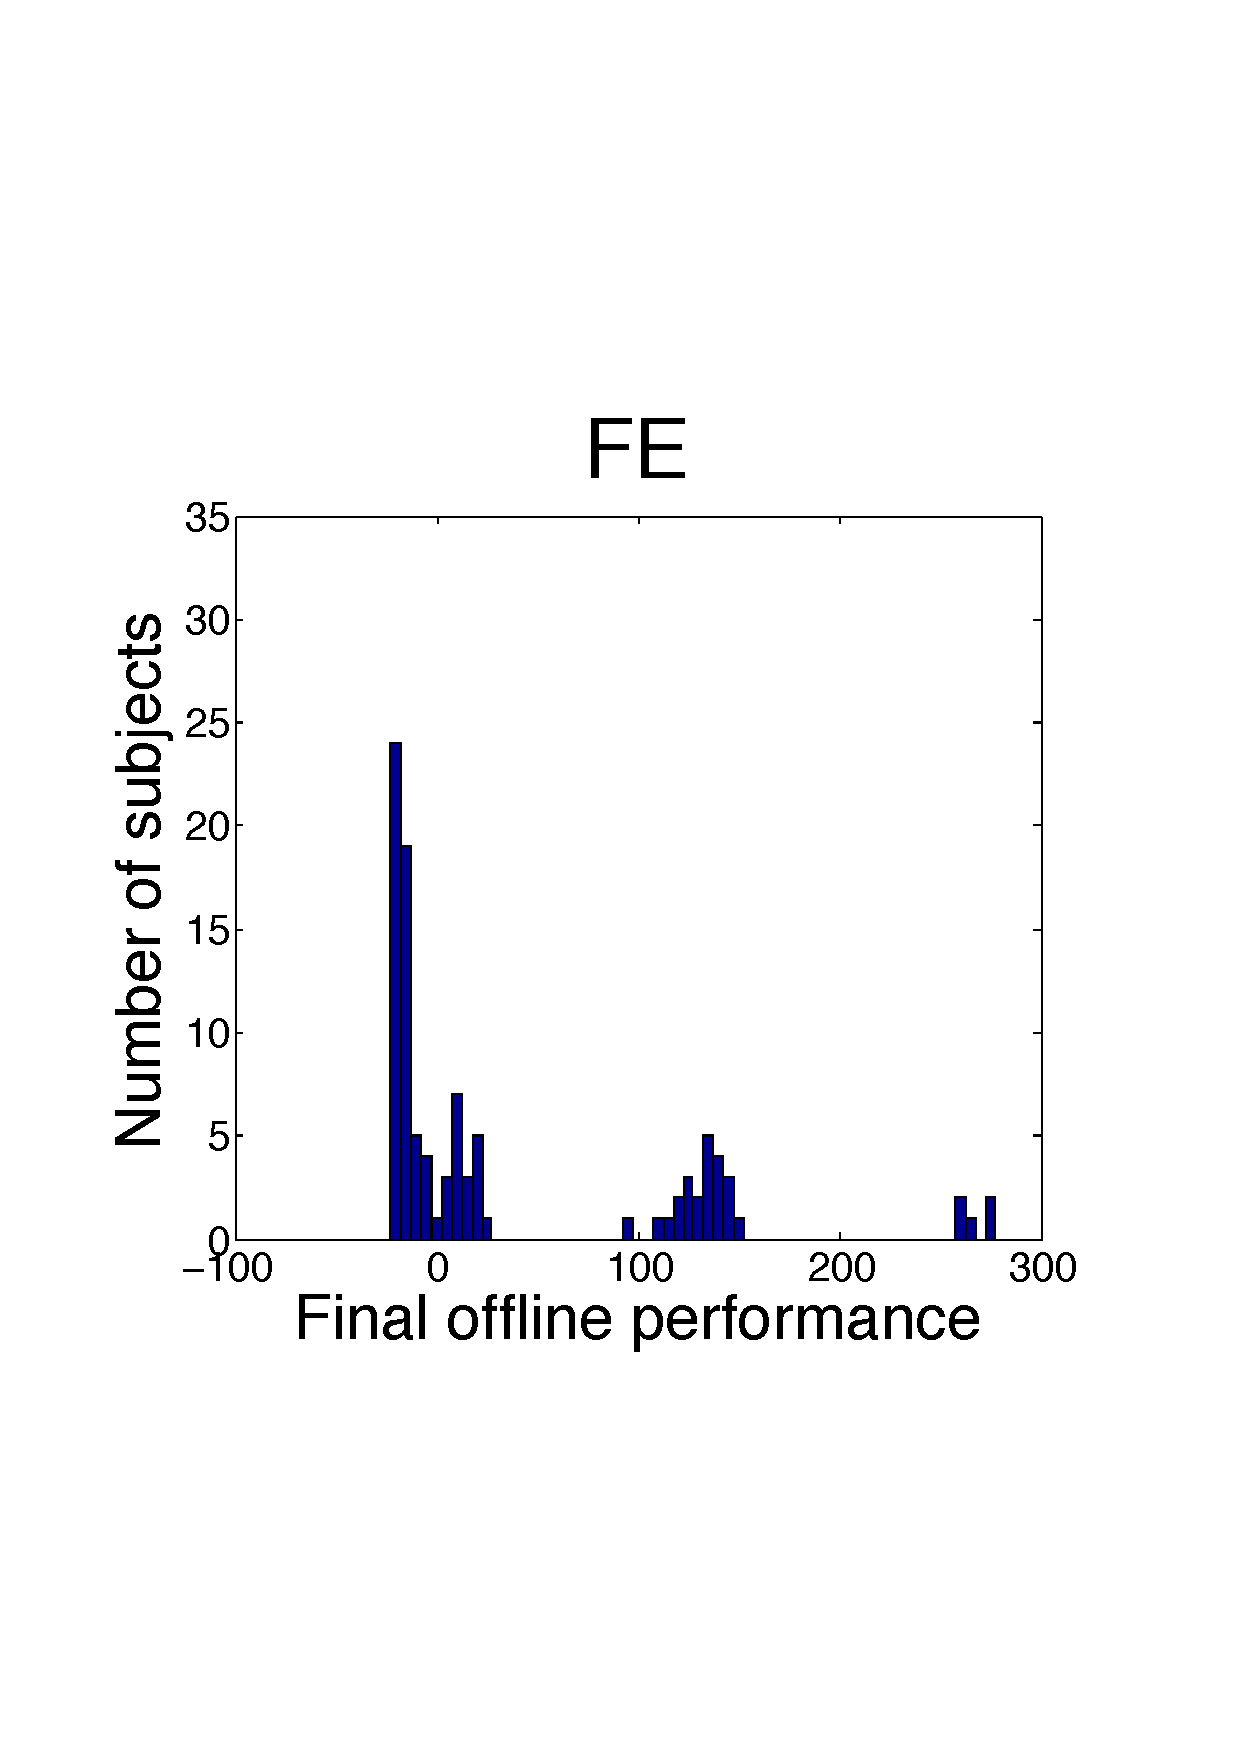
\includegraphics[width=0.47\columnwidth]{DistributionFinalOfflinePerformFE.pdf}&
\includegraphics[width=0.47\columnwidth]{DistributionFinalOfflinePerformCompetitive.pdf}&
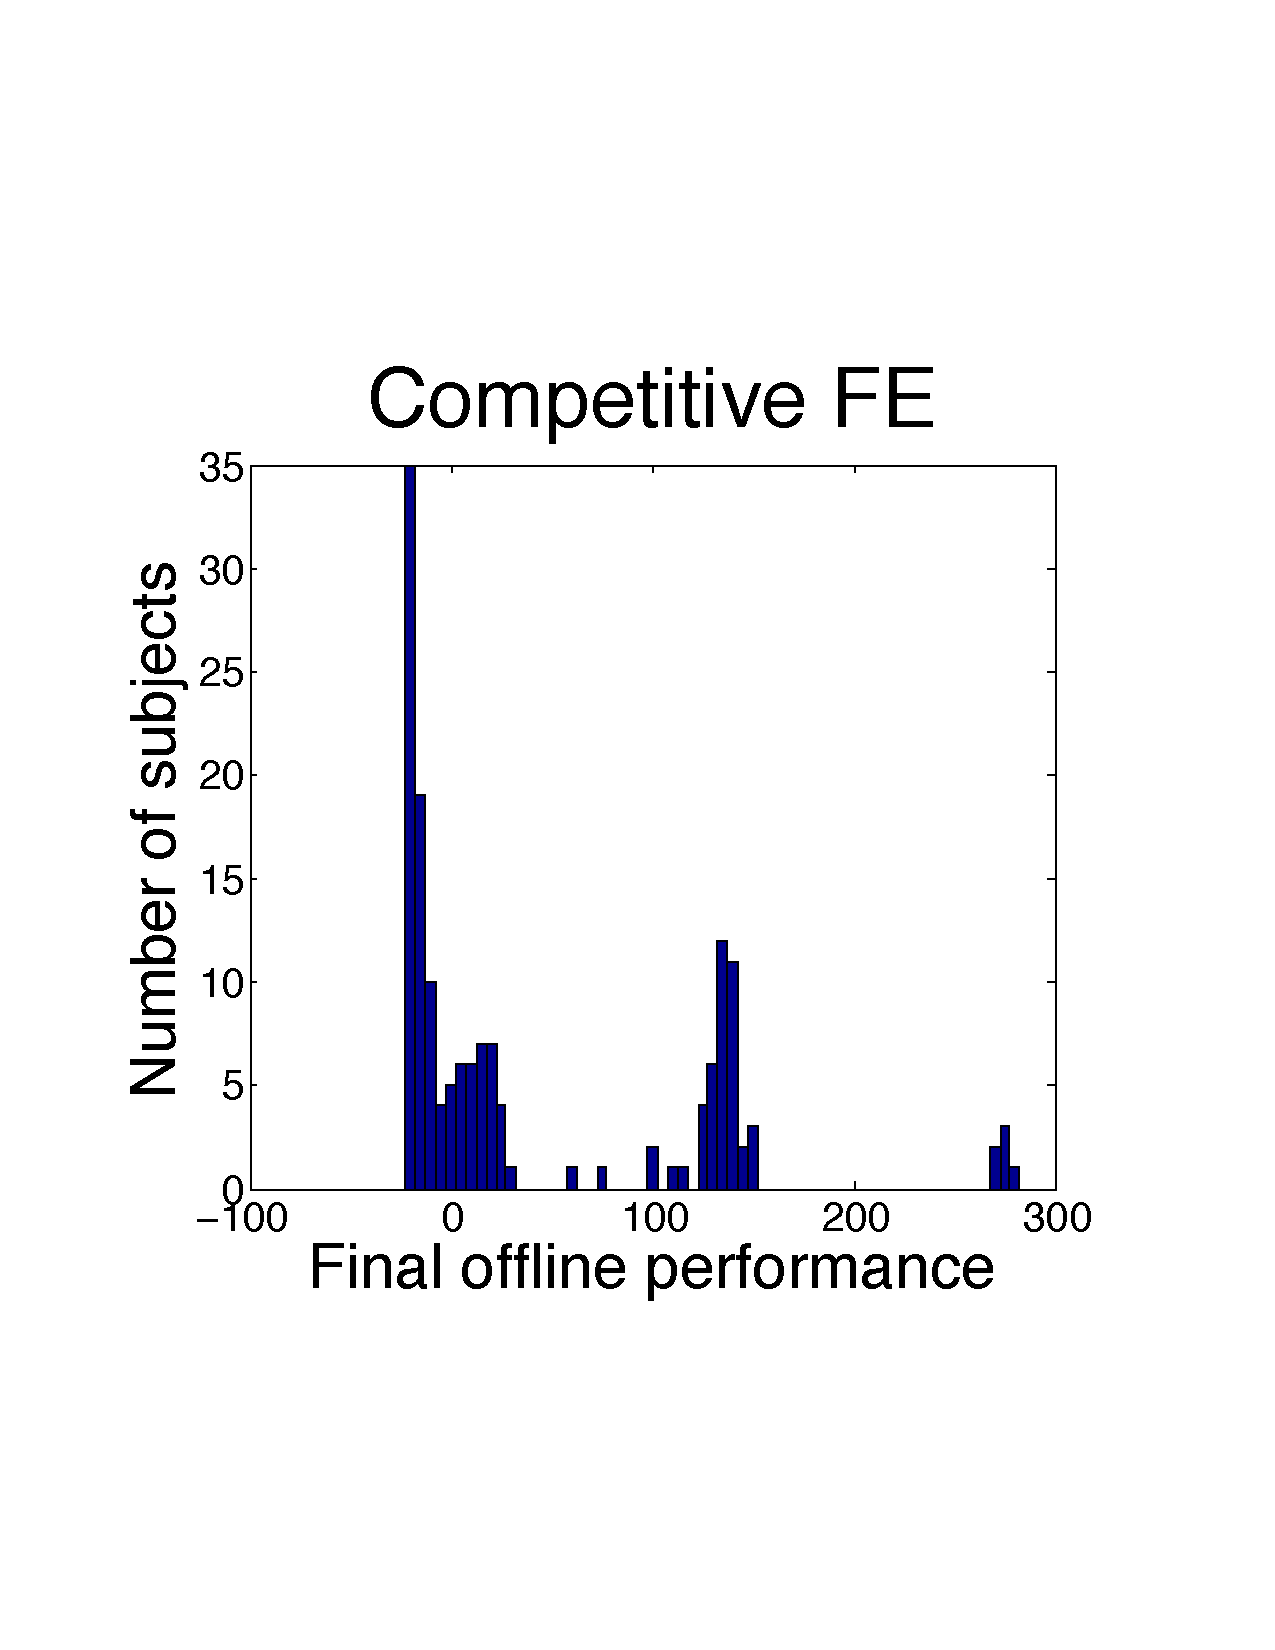
\includegraphics[width=0.47\columnwidth]{DistributionFinalOfflinePerformCompetitiveFE.pdf}
%(a)&(b)&(c)&(d)\\
%\vspace{-2mm}
\end{tabular}
\caption{Distribution of final offline performance across the four conditions. FE=Facial Expression.}%: a) Control condition, b) FE condition, c) Competitive condition and d) Competitive FE condition (FE=Facial Expression). %\HH{Could it make sense to actually color the bars here according to the highlest level that was reached for a given bar? It might help in better expalaining the multi-level scoring}}
%\vspace{-2mm}
\label{HisFinalOfflinePerformance}
\end{figure*}

\subsection{Feedback Given}

Figure \ref{feedback} shows how feedback was distributed per 200 time steps over the learning process for the four conditions. From Figure \ref{feedback} we can see that the number of time steps with feedback received by agents in the four conditions increased at the early training stage and decreased dramatically afterwards, which supports previous studies \cite{knox2012humans,li2013using} and our motivation for investigating methods of enabling agents to learn from the trainer's facial expressions. In addition, the number of feedback received by agents in the competitive and competitive facial expression condition is more than that in the control and facial expression conditions before 1000 time steps, which shows that the agent's competitive feedback can increase the number of feedback given by the trainer. %at least at the early training stage.

%Trainers in both informative conditions gave feedback for much longer than those in the control condition. Most notably, trainers in the uncertainty-informative condition gave a strikingly large amount of feedback, even during later intervals, with a much slower fall-off than the other conditions.

%%Figure \ref{feedback} 
%Our results show that both  `facial expression' and `competition' increase the amount of feedback given via key presses, though not significantly.
%%telling subjects to use facial expressions as a separate channel for giving feedback to train agents increases the amount of feedback given via key presses, and an agent's competitive feedback can also increase the amount of feedback given by the trainers even at a much broader age range (from 6 to 72) than was considered in \cite{li2014learning}, though not significantly. 
%However, Figure \ref{control&feedback}b shows that the higher the level the agents reach, the less feedback they receive ($F(2,490) = 9.11, p = 0.0001, \eta_{p}^{2} = 0.036$). 

%the mean number of time steps with feedback with and without  `facial expression' and `competition'. %summarizes the mean and median number of time steps with feedback for each condition. %\HH{Doesn't one time step equates to a certain number of ticks which is independent of when actions of the agent are taken...?} 
%One time step equates to the execution of one action by the agent. The results show that, `facial expression' does not decrease the number of time step with feedback provided by trainers ($F[1,492]$ = $0.57$, $p$ = $0.45$, $\eta_{p}^{2}$ = $0.001$), %($F[1,492] = 0.57, p = 0.4504, \eta_{p}^{2} = 0.0012$), 
%and `competition' increased the number of time step with feedback provided by trainers ($F[1,492]$ = $1.37$, $p$ = $0.24$, $\eta_{p}^{2}$ = $0.003$). 
%($F[1,492] = 1.37, p = 0.2426, \eta_{p}^{2} = 0.0028$). %in terms of both mean and median, in the competitive condition, trainers gave more feedback than those in the control condition ($p = 0.075$). Similarly, in the competitive facial expression condition, trainers gave more feedback than those in the facial expression condition ($p = 0.2298$). However, trainers in the facial expression condition and competitive facial expression condition gave similar amounts of feedback to those in the control and competitive conditions respectively.% ($p = 0.2842$ and $p = 0.5439$ respectively). \sw{What do these p-values mean?  Was the null hypothesis here that they were the same or different?}

%Overall, our results show that telling the subjects to use facial expressions as a separate channel for giving feedback for training agents does not decrease the amount of feedback given via key presses, and an agent's competitive feedback can increase the amount of feedback given by the trainers even at a much broader age range (from 6 to 72) than was considered in \cite{li2014learning}, though not significantly.

%provide additional evidence that, even at a much broader age range (from 6 to 72) than was considered in \cite{li2014leveraging}, an agent's competitive feedback can increase the amount of feedback given by the trainers. Moreover, telling the subjects to use facial expressions as a separate channel for giving feedback for training agents does not decrease the amount of feedback given via key presses.





%\vspace{-3mm}
%\paragraph{Performance}
\subsection{Performance}
\label{sec:per}

%\begin{figure}[tb]
%%\vspace{-2mm}
%%\hspace{4mm}
%\centering
%\includegraphics[width=0.7\columnwidth,trim=0 0 0 0, clip]{MeanOfflinePerformancePerEpisode} 
%\vspace{-2mm}
%\caption{Mean offline performance per episode trained by one of the authors.}
%\vspace{-4mm}
%\label{MeanOfflinePerformanceEpisode}
%\end{figure}

%First, to see whether a TAMER agent can successfully learn to play the game and compare the learning performance with other methods, one of the authors trained the agent on difficulty level 0 with seed 121 \HH{I dont' recall any prior mention of the difficulty level or seed. If this is important, then you should also mention this in the experimental set up.} in the Infinite Mario Domain for 10 trials with TAMER. %Figure \ref{setup&feedback&performance}c shows the average offline performance per episode. 
%We take a dying of Mario and finishing the level as one episode. The policy was frozen and recorded at the end of each episode of training. Then, each policy was tested for 20 games offline. The performance for each episode %in Figure \ref{setup&feedback&performance}c 
%was averaged over the 20 games and then over the 10 trials. The result shows that our TAMER agent can achieve 120 points in 12 episodes, while it takes about 500 episodes for a SARSA agent to achieve a similar performance level \cite{taylor2011teaching} and a hierarchical SARSA agent implemented with object-oriented representation 300 episodes to achieve 149.48 points \cite{mohan2011object}, which is almost optimal. Although the TAMER agent does not learn an optimal policy, it can successfully learn a good policy substantially faster than these other methods, making this set-up very suitable for our experiments with members of the public where each training session can only last up to 15 minutes. %\HH{It's great that you did this. Very good!} 
%\HH{I wonder if this part would be better described in the experimental set up. This part isn't really a result in itself but a way of showing that we did some serious experimental preparation to verify the efficacy of the set up. }


%
%To see whether the agent's competitive feedback can motivate a human trainer to give better feedback and ultimately improve the agent's learning, we examined how the agent's performance varied as its policy changed over time in the four conditions. We divided the whole training process into intervals, with each interval composed of 200 time steps. As before, the agent's policy was frozen and tested offline for 20 games and performance was averaged across all subjects within each condition. However, some factors such as the distribution of the trainer's skill level across conditions, the domain stochasticity etc., may still affect the evaluation of agent performance. Nonetheless, we believe that the large number of participants in our study can partially compensate for these variabilities. 
%
%Our results show that an agent's competitive feedback can motivate human trainers to train agents better regardless of whether they are told to use facial expressions as a separate channel to train the agent or not. As shown in Figure \ref{finalofflineperformance}, agents in the competitive condition ultimately outperform those in the control condition, especially in terms of the median ($p = 0.2952$). Similarly, agents in the competitive facial expression condition ultimately outperform those in the facial expression condition ($p = 0.2096$). Moreover, agents in the facial expression condition and competitive facial expression condition ultimately perform worse than those in the control and competitive condition respectively ($p = 0.2072$ and $p = 0.2827$). %\sw{Discuss why the mean and median are so different.}
%
%In summary, our results verify that the agent's competitive feedback can improve its performance. In addition, the results are consistent with our hypothesis that telling the subject to use facial expressions as a separate channel to give feedback has a negative effect on the agent's learning.
%
%However, the mean and median performance are quite different and the differences between conditions are not statistically significant. 

%see whether the agent's competitive feedback and telling to use facial expressions as separate channel have effect on agent learning and 
To get some exploratory insights into our data, we first analyzed the distribution of final offline performance for each condition with the learned final policy tested offline for 20 games and averaged over the 20 games for each subject. %as shown in Figure \ref{HisFinalOfflinePerformance}. 
Figure \ref{HisFinalOfflinePerformance}, which contains histograms of the final offline performance for the four conditions, shows that the distribution in the four conditions are all characterized by three modes. The gap between modes is caused by the score mechanism which gives credit +100 for finishing one level and much less otherwise. Therefore, the three modes in Figure \ref{HisFinalOfflinePerformance} from left to right correspond to level 0, 1 and 2 in the game respectively.

%\HH{It's really strange to say this and not give any explanation of why! By the way, the following sentence provides an observation but not explanation for this result. Why dont' you include something about the level number that was reached for each mode?}.  
%In each condition, many subjects' agents performed poorly, with scores below 50, reflecting a failure to master basic skills.  A moderate number of subjects' agents performed solidly, with scores around 125, on par with the agent we trained. %(see Figure \ref{setup&feedback&performance}c).  
%A small number of subjects' agents performed exceptionally, with scores in excess of 250.  


%\begin{figure*}[htb]
%%\vspace{-2mm}
%%\hspace{4mm}
%\centering
%%\begin{tabular}{c c c}
%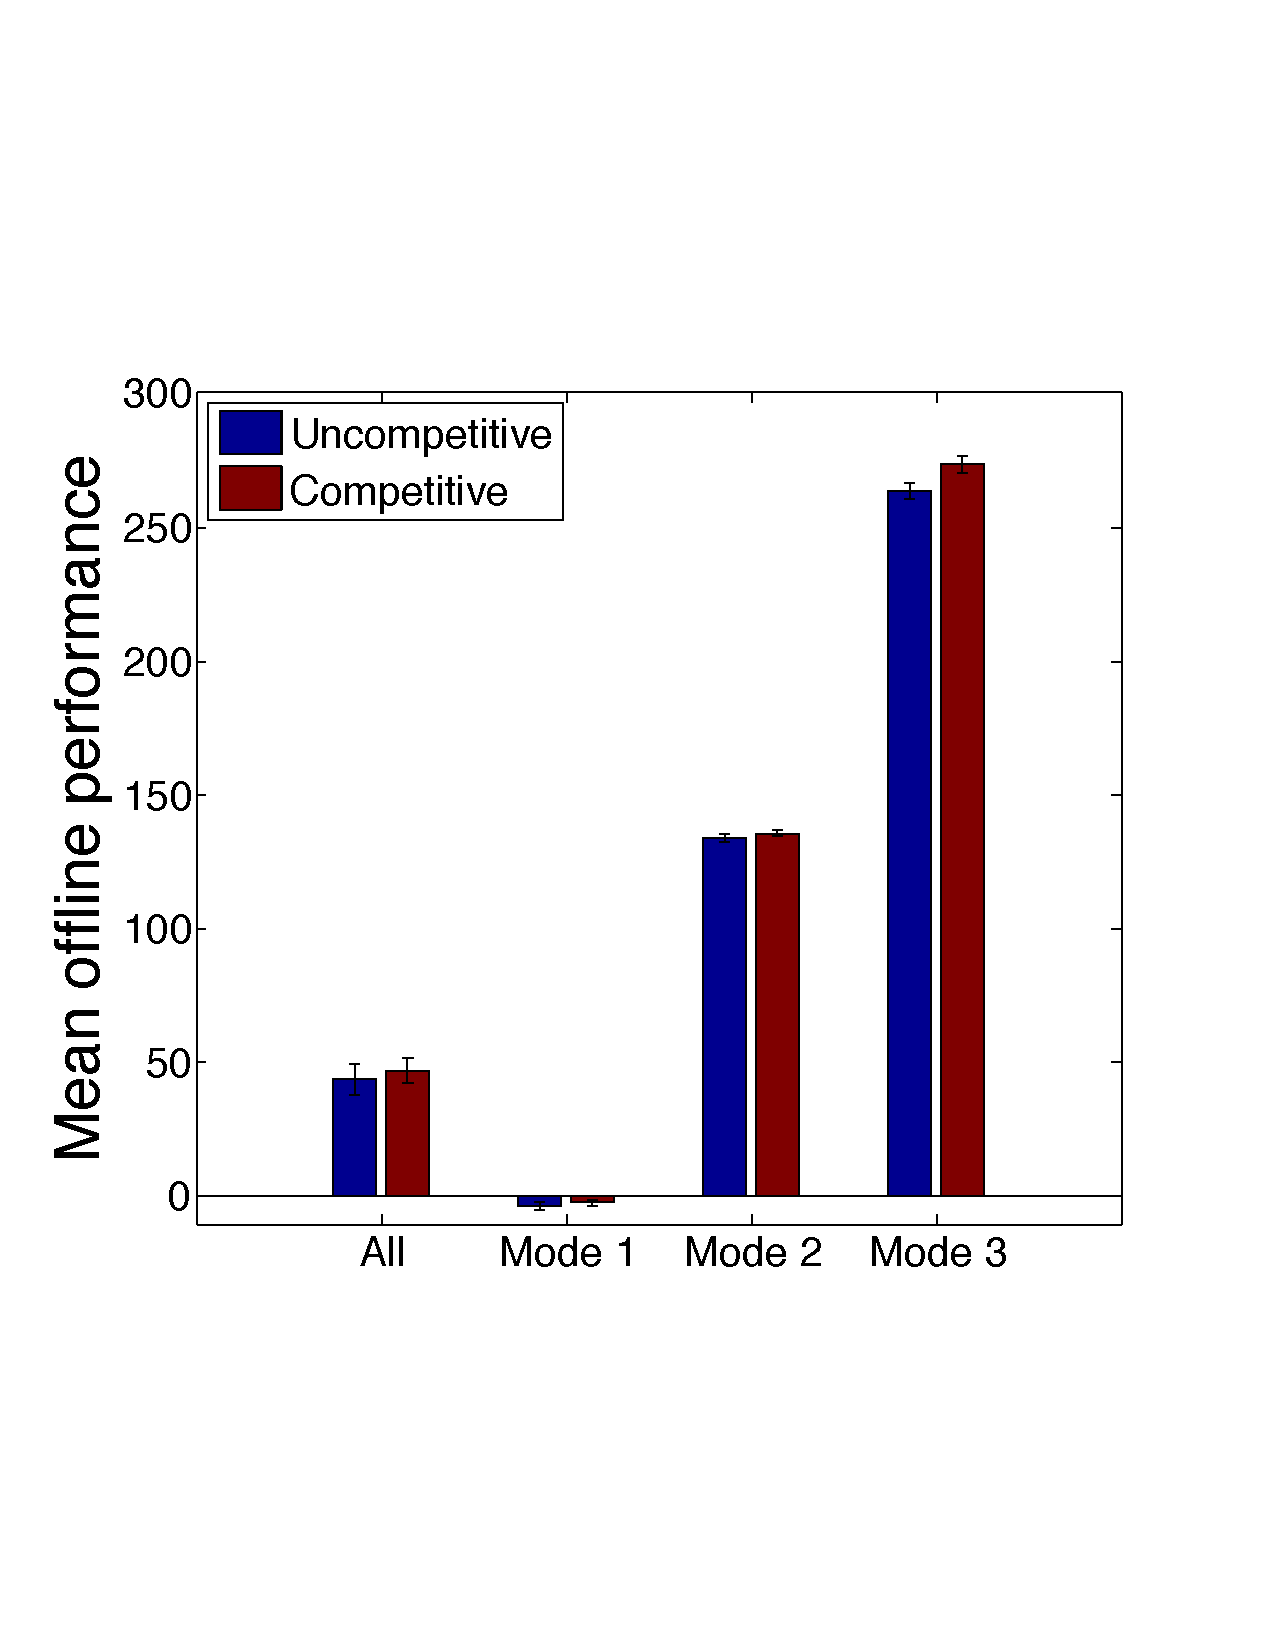
\includegraphics[width=0.75\columnwidth,trim=0 0 0 0, clip]{CompetitionPerMode}&
%\includegraphics[width=0.45\columnwidth,trim=0 0 0 0, clip]{FacialExpressionPerGender}&
%%\includegraphics[width=0.5\columnwidth,trim=0 0 0 0, clip]{CompetitionPerGender}&
%\includegraphics[width=0.60\columnwidth,trim=0 0 0 0, clip]{CompetitionPerAge} \\
%%\vspace{-2mm}
%(a)&(b)&(c)
%\end{tabular}
%\vspace{-4mm}
%\caption{Mean final offline performance for a) agents across and within mode 1, 2, 3 distributed in Figure \ref{HisFinalOfflinePerformance} from left to right trained with and without competitiveness, b) agents trained by female and male subjects with and without facial expression, and c) agents trained by trainers in three age groups with and without competitiveness. Note: black bars stand for standard error. %and mode 1 corresponding to the left mode (level 0), mode 2 corresponding to the middle mode (level 1) and mode 3 corresponding to the right mode (level 2) in a).
%}
%\vspace{-5mm}
%\label{performance}
%\end{figure*}

%The histograms highlight a similar distribution in both competitive conditions and between both non-competitive conditions.
%% the competitive and competitive facial expression conditions, and in conditions. %also show that the distribution of final offline performance in the competitive condition and competitive facial expression condition are similar, while the distributions of final offline performance in the control and facial expression condition are also similar. 
%Although the number of subjects who trained the agent well 
%%\HH{ be careful with the use of a word that implies time dependence...}
%% increased 
%was higher (increased by 32)
%because of the competitive element in the corresponding condition, 
%% competitiveness in the competitive and competitive facial expression conditions, 
%the number of subjects who trained agents poorly was 
%% high or 
%%\HH{ be careful with the use of a word that implies time dependence...}
%% also increased. 
%similarly high (increased by 49). %\HH{ if you want to talk about similar or higher values, you really need to provide numerical evidence. These statements about the quantative are currently too qualitative...}



%This may partially explain the large difference between mean and median performance and the lack of significance in the performance differences between conditions.
%\HH{Nice!}

%Given there are three modes in the distribution of final offline performance and a broad range of ages and genders across trainers, to get a deep insight of the data, we consider mode of the final offline performance as an additional factor in the n-way ANOVA test.% in terms of five factors: , 
%facial expression, competition, age and gender. Here `facial expression' means whether telling trainers to use facial expression to train the agent or not, %as in the facial expression condition and competitive facial expression condition, 
%while `competition' means whether there is leaderboard in the training interface.% as in the competitive condition and competitive facial expression condition. 
%`Gender' and `age' mean all trainers were divided into females and males and three age groups: under 13, 13 to 30 and older than 30 years old. 

%\begin{table}[htb]
%%\renewcommand{\arraystretch}{1.5}
%%\captionsetup{font=footnotesize}
%
%\centering
%\begin{tabular}{ r | l | l | l }
%\toprule
%%\multirow{2}{*}{Condition} &Non-social  &  Social behavior \\
%& \textbf{Mode 1} & \textbf{Mode 2}  & \textbf{Mode 3}\\
%\toprule
%\textbf{Competition} & $p = 0.1271$ & $p$ = $\textbf{0.0334}^{\ast}$ & $p$ = $\textbf{0.0135}^{\ast}$ \\
%\hline
%\textbf{Gender} & $p = 0.3777$ & $p = 0.6141$ &  $p = 0.6055$ \\
%\hline
%\textbf{Age} & $p = 0.4726$ & $p = 0.4032$ & $p = 0.2069$\\
%\hline
%\textbf{FE} & $p = 0.5098$ & $p = 0.8976$ & $p = 0.2482$ \\
%\toprule
%\end{tabular}
%\caption{ANOVA test of factor effect on final agent performance for the three performance modes shown in Figure \ref{HisFinalOfflinePerformance}. Note: mode 1 corresponding to the left mode, mode 2 corresponding to the middle mode and mode 3 corresponding to the right mode in Figure \ref{HisFinalOfflinePerformance}. $^{\ast}$Statistically significant.}
%%\vspace{-4mm}
%\label{mode}
%\end{table}

\begin{figure}[htb]
\vspace{4mm}
%\hspace{4mm}
\centering
%\begin{tabular}{c c c}
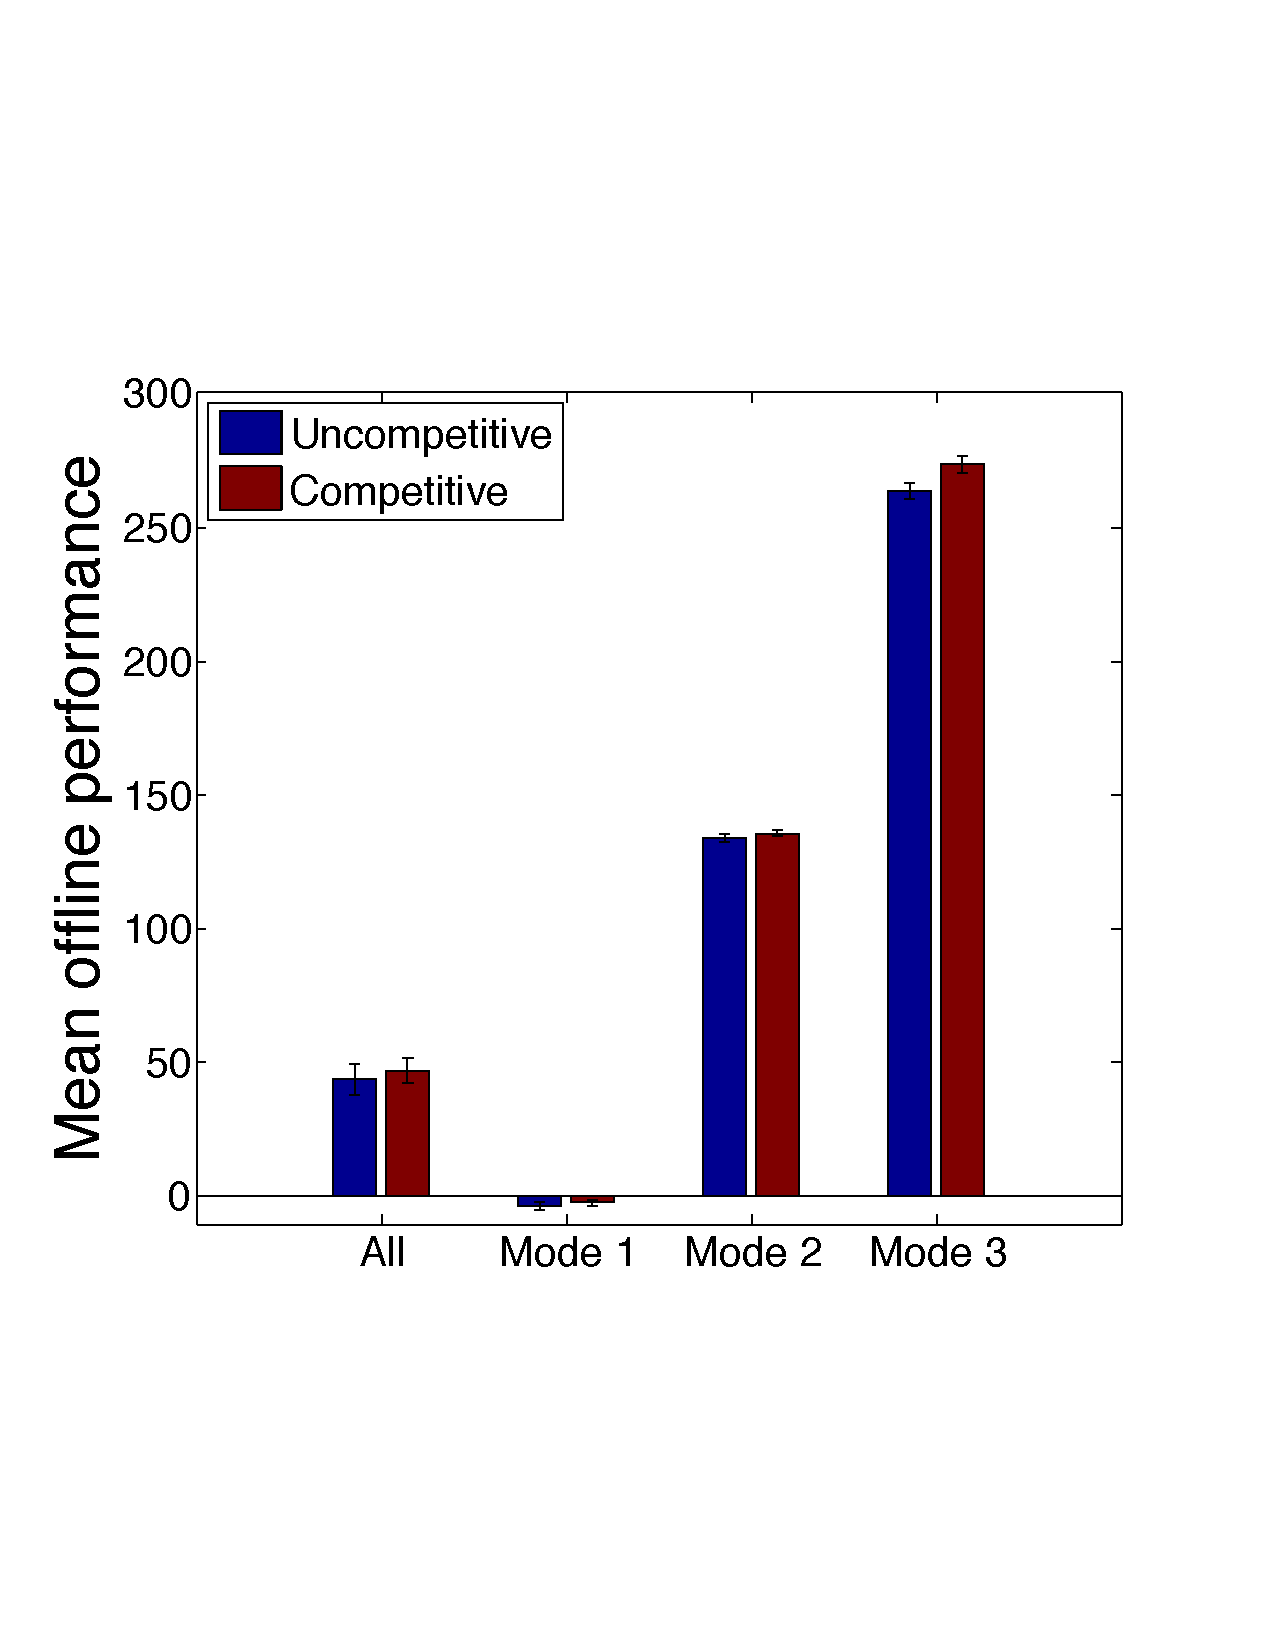
\includegraphics[width=0.8\columnwidth, trim=0 0 0 0, clip]{CompetitionPerMode}%&
%\includegraphics[width=0.38\columnwidth, height=1.56in, trim=0 0 0 0, clip]{FacialExpressionPerGender}&
%\includegraphics[width=0.50\columnwidth, height=1.56in, trim=0 0 0 0, clip]{CompetitionPerAge} \\
%(a)&(b)&(c)
%\end{tabular}
%\vspace{2mm}
\caption{Mean final offline performance for agents across and in the three modes distributed in Figure \ref{HisFinalOfflinePerformance}, trained with and without competitiveness. % trained by (b) female and male subjects with and without facial expression, (c) trainers in three age groups with and without competitiveness. 
Note: black bars stand for standard error.}
\vspace{4mm}
\label{Mode}
\end{figure}


%Given there are three modes in the distribution of final offline performance with a large difference in performance, %and a broad range of ages and genders across trainers, 
%to get a deep insight of the data, 
%we consider the mode of the final offline performance as an additional factor in the $n$-way ANOVA test.  
%\HH{how can you consider a mode as an additional factor? This doesn't make sense. You probably have to assign an integer to label a particular mode. However, you need to do this systematically. How was this determined? Why aren't you talking about the highest level that mario reached? The way you describe it now seems like you numbered the start and end of each node manually yourself... which is not what I had discussed with you before....You remember after my discussion with the psychologists in Eindhoven that you should consider splitting the modes based on the maximum level surpassed?I'm surprised that you have not written this anyway. It makes me rather concerned that you present here the experiments from the analysis that you already did before the submission of last year's aamas submission...}. 
Figure \ref{Mode} highlights the importance of `competition'. %for all agents and agents distributed in the three modes in Figure \ref{HisFinalOfflinePerformance}. %When taking all five factors together, %the results show that %the mode of the final offline performance has a significant role on agent learning performance ($p = 0$), which is obviously and clearly shown in Figure \ref{HisFinalOfflinePerformance}, and 
For all agents across all modes, Figure \ref{Mode} shows that `competition' can motivate trainers to train agents  significantly better ($F(1,471)$ = $4.45$, $p$ = $0.035$, $\eta_{p}^{2}$ = $0.009$). %($F[1,490] = 5.33, p = 0.0214, \eta_{p}^{2} = 0.0108$). %while `age' and `gender' factors have insignificant effect on agent final performance ($F[2,490] = 1.47, p = 0.2307, \eta_{p}^{2} = 0.006$ and $F[1,490] = 0.98, p = 0.3223, \eta_{p}^{2} = 0.002$, respectively). 
%Moreover, when looking into the interaction between the five factors, we found that the interaction of `facial expression' and `gender' has a significantly negative effect on agent performance ($F[1,471]$ = $5.06$, $p$ = $0.02$, $\eta_{p}^{2}$ = $0.011$). %($F[1,471] = 5.06, p = 0.0249, \eta_{p}^{2} = 0.0106$). 
While examining %the factor effect for 
each mode, %as shown in Table \ref{mode}, 
Figure \ref{Mode} shows that `competition' can significantly improve the agent's learning in %mode 2 ($F[1,116]$ = $4.64$, $p$ = $0.03$, $\eta_{p}^{2}$ = $0.015$) and 
mode 3 ($F(1,19)$ = $7.41$, $p$ = $0.01$, $\eta_{p}^{2}$ = $0.04$),  %($F[1,116] = 4.64, p = 0.0334, \eta_{p}^{2} = 0.0152$) and mode 3 ($F[1,19] = 7.41, p = 0.0135, \eta_{p}^{2} = 0.0399$) 
%respectively, %corresponding to the middle and right modes in Figure \ref{HisFinalOfflinePerformance} 
in which agents performed best. However, when examining `facial expression', there is no effect on agents' learning across modes or within each mode.


%\begin{figure}[htb]
%%\vspace{-2mm}
%%\hspace{4mm}
%\centering
%%\begin{tabular}{c c}
%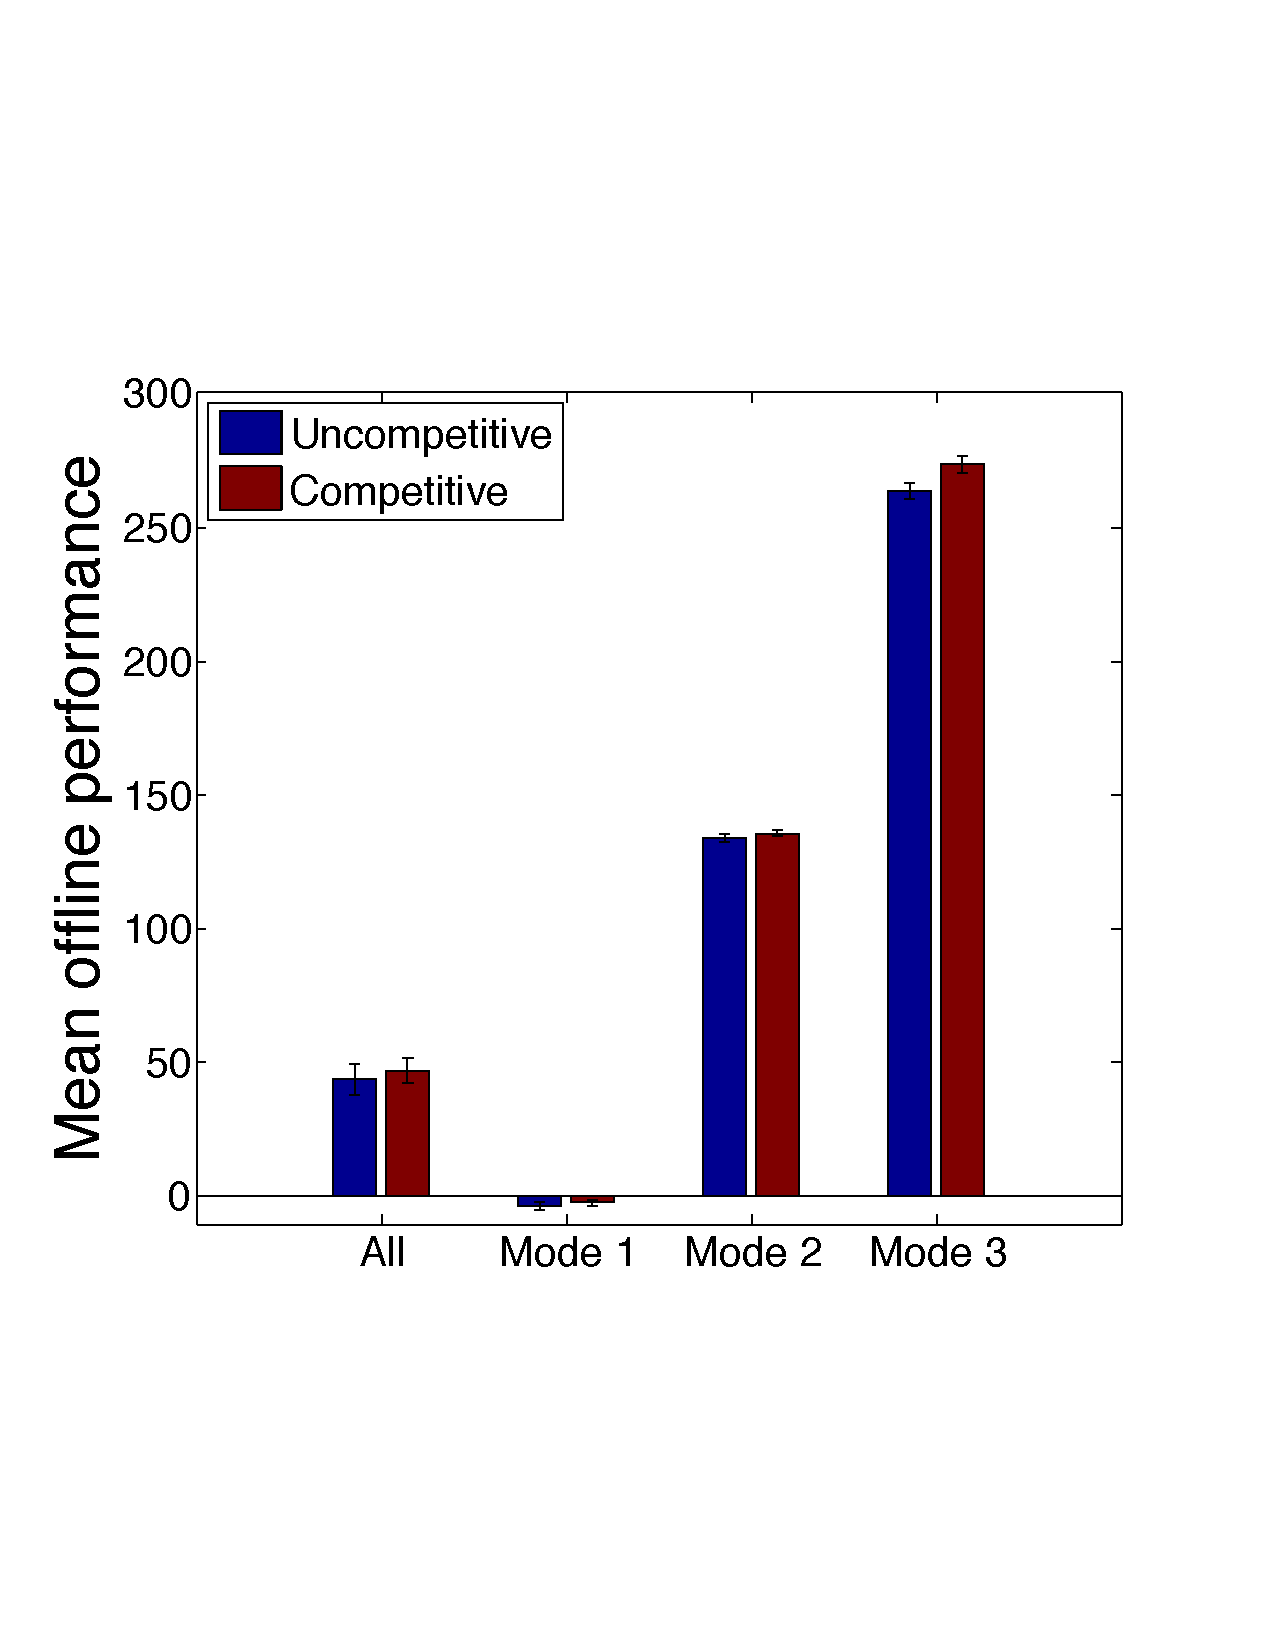
\includegraphics[width=0.75\columnwidth,trim=0 0 0 0, clip]{CompetitionPerMode}
%%\includegraphics[width=0.495\columnwidth,trim=0 0 0 0, clip]{MedianOfflinePerformance} \\
%%a&b
%%\end{tabular}
%\vspace{-4mm}
%\caption{Mean final offline performance for agents across and in the three modes distributed in Figure \ref{HisFinalOfflinePerformance}, trained with and without competitiveness. Note: black bars stand for standard error.}%mode 1 corresponding to the left mode (level 0), mode 2 corresponding to the middle mode (level 1) and mode 3 corresponding to the right mode (level 2) in Figure \ref{HisFinalOfflinePerformance}. }
%\vspace{-4mm}
%\label{mode}
%\end{figure}

%especially while trained by good trainers. 
%However, though the results are significant, differences between the mean performances are not large. We believe that it could be because of the inappropriate reward for easy and difficult agent's behaviors by the score mechanism.%who can train agents to perform better. %While our results also show that the interaction of `facial expression' and `gender' has a significant negative effect on agent performance, we are curious to know how `facial expressions' and `competition' affect different genders and age groups.

In addition, we found that there is a two-way interaction between `facial expression' and `gender':  
`facial expression' has a significantly negative effect on agent learning trained by female trainers ($F(1,185)$ = $4.57$, $p$ = $0.03$, $\eta_{p}^{2}$ = $0.024$) but not by male ones. When looking into each mode in Figure \ref{HisFinalOfflinePerformance}, we found that within mode 1 (level 0 in the game), %agents trained by female trainers performed significantly better than by males ones %a significant effect on agent's learning performance was caused by `gender' 
%($F(1,332)$ = $4.07$, $p$ = $0.045$, $\eta_{p}^{2}$ = $0.012$) and %there is a two-way interaction between `facial expression' and `gender': 
`facial expression' ruins agent learning trained by female subjects ($F(1,332)$ = $6.75$, $p$ = $0.01$, $\eta_{p}^{2}$ = $0.02$). However, we found no significant gender-specific effect of `competition' on training.

Moreover, while examining the `age', we found that `competition' can significantly motivate trainers older than 30 to train the agent better ($F(1,123)$ = $4.65$, $p$ = $0.03$, $\eta_{p}^{2}$ = $0.036$)  %not trainers younger than 30 years old. %under 13 years old ($F[1,241]$ = $2.99$, $p$ = $0.085$, $\eta_{p}^{2}$ = $0.012$), %($F[1,241] = 2.99, p = 0.0848, \eta_{p}^{2} = 0.0123$), 
%though not significant. 
but not %has no effect on trainers 
those younger than 30. %While examining `facial expression'
Furthermore, we found that %it has some negative effect on agent training by subjects older than 30 years old ($F(1,123)$ = $2.42$, $p$ = $0.12$, $\eta_{p}^{2}$ = $0.019$), %($F[1,123] = 2.42, p = 0.1225, \eta_{p}^{2} = 0.0193$), 
%and %
there is a two-way interaction between `facial expression' and `gender' for trainers younger than 13 years old: `facial expression' 
ruins agent learning trained by female participants younger than 13 ($F(1,232)$ = $7.1$, $p$ = $0.008$, $\eta_{p}^{2}$ = $0.03$).


Overall, these results support prior results \cite{li2014learning} demonstrating the importance of bi-directional interaction and competitive elements in the training interface, and show that `competition' can significantly improve agent learning and help the best trainers the most. Moreover, our results show that %`facial expression' -- telling subjects to use facial expressions as a separate training channel has some effect on final agent performance trained by subjects older than 30 years old and
`competition' can significantly motivate participants older than 30 to train agents better not those who are younger.
In addition, our results suggest that `facial expression' %telling subjects to use facial expressions as a separate training channel 
has a significantly negative effect on agent training by female participants, especially those who are less than 13 years old and cannot train agents to perform well. %that can only reach level 0 most frequently, % not by male trainers, 
%and `competition' has no effect on agent training by males and females respectively. 
%Moreover, our results show that %`facial expression' -- telling subjects to use facial expressions as a separate training channel has some effect on final agent performance trained by subjects older than 30 years old and
%`competition' can significantly motivate subjects older than 30 years old to train agent better not those younger ones. %than 30 years old. 
%Furthermore, %for trainers between 13 and 30 years old, agents trained by male subjects performed better than those by female ones and %the two-way interaction effect was on trainers younger than 13 years old.
% %telling to use facial expression as a separate training channel 
%`facial expression' has a negative effect on agent learning trained by female subjects younger than 13 years old.

%\begin{table}
%%\renewcommand{\arraystretch}{1.5}
%%\captionsetup{font=footnotesize}
%\centering
%\begin{tabular}{ r | l | l }
%\toprule
%%\multirow{2}{*}{Condition} &Non-social  &  Social behavior \\
%& \textbf{Female} & \textbf{Male}  \\
%\toprule
%\textbf{Perfor. mode} & $p$ = $\textbf{0}^{\ast}$ & $p$ = $\textbf{0}^{\ast}$ \\
%\hline
%\textbf{Competition} & $p = 0.4881$ & $p$ = $\textbf{0.007}^{\ast}$ \\
%\hline
%\textbf{Age} & $p$ = \textbf{0.076} & $p = 0.9655$\\
%\hline
%\textbf{FE} & $p$ = $\textbf{0.0339}^{\ast}$ & $p = 0.2039$ \\
%\toprule
%\end{tabular}
%\caption{ANOVA test of factor effect on final agent performance for female and male subjects. $^{\ast}$Statistically significant.}
%%\vspace{-4mm}
%\label{gender}
%\end{table}

%\sw{We also need something here to support our claim that the results show TAMER can be used to learn Mario.  How do these average scores compare to RL benchmarks after the same number of episodes?  What kind of qualitative performance do they correspond to?  Can we argue that Mario was able to master basic skills due to TAMER training?}

%\HH{What happened to the learning curves? Can we include some of them? The dip in learning was something that could be discussed.. and how it varies across gender/age...?}


%\vspace{-3mm}
%\paragraph{Role of Gender}
%\subsection{Role of Gender}
%\begin{figure*}[htb]
%%\vspace{-2mm}
%%\hspace{4mm}
%\centering
%\begin{tabular}{c c}
%\includegraphics[width=0.8\columnwidth,trim=0 6 10 10, clip]{FinalOfflinePerformanceForFemale} &
%\includegraphics[width=0.8\columnwidth,trim=0 6 10 10, clip]{FinalOfflinePerformanceForMale}\\
%a&b
%\end{tabular}
%\caption{Final offline performance for female (a) and male (b) subjects. (FE=Facial Expression.)}
%\label{FinalOfflinePerformanceGender}
%\end{figure*}



%While our results show that competitive feedback can significantly improve agent final performance, %that the interaction of `facial expression' and `gender'  has significantly negative effect on the agent performance. %motivate human trainers to give better feedback and improve the agent's ultimate performance.  
%%telling trainers to use facial expressions as a separate channel to give feedback 
% %has a negative effect on the agent's learning. 
%%Moreover, 
%%When looking into the interaction between the five factors, we found that the interaction of `facial expression' and `gender' has a significantly negative effect on agent performance ($F[1,471]$ = $5.06$, $p$ = $0.02$, $\eta_{p}^{2}$ = $0.011$).
%we wanted to know which gender `competition' and `facial expression' affect more, since females and males often perceive and react to social situations differently, e.g., girls have been shown to be significantly more relationally aggressive than boys \cite{crick1995relational}.
%%Moreover,

%We found that %there is a two-way interaction between `facial expression' and `gender':  
%`facial expression' has a significantly negative effect on agent learning trained by female trainers ($F(1,185)$ = $4.57$, $p$ = $0.03$, $\eta_{p}^{2}$ = $0.024$) but not by male ones, as shown in Figure \ref{ModeGengerAge}b.
%%($F(1,471)$ = $6.49$, $p$ = $0.01$, $\eta_{p}^{2}$ = $0.014$). 
%When looking into each mode in Figure \ref{HisFinalOfflinePerformance}, we found that within mode 1 (level 0 in the game), %agents trained by female trainers performed significantly better than by males ones %a significant effect on agent's learning performance was caused by `gender' 
%%($F(1,332)$ = $4.07$, $p$ = $0.045$, $\eta_{p}^{2}$ = $0.012$) and %there is a two-way interaction between `facial expression' and `gender': 
%`facial expression' ruins agent learning trained by female subjects ($F(1,332)$ = $6.75$, $p$ = $0.01$, $\eta_{p}^{2}$ = $0.02$). % in mode 1 (level 0 in the game).
%Moreover, we found no significant gender-specific effect of `competition' on training.


%Therefore, we want to know which gender `facial expression' and `competition' affect more, since females and males often perceive and react to social situations differently, e.g., girls have been shown to be significantly more relationally aggressive than boys \cite{crick1995relational}. %We hypothesize that the effect of competitive feedback would be different for male and female subjects, since they often perceive and react to social situations differently, e.g., girls have been shown to be significantly more relationally aggressive than boys \cite{crick1995relational}.  %\HH{removing this citation. i don't see the link..venkatesh2000don} %\sw{Need supporting cites here}. 
%Therefore, we analyzed the offline performance for male and female subjects across the four conditions.
%
%Therefore, we did n-way ANOVA test with the other four factors on agent final performance for female and male subjects separately.% as shown in Table \ref{gender}.
%
%From Table \ref{gender} we can see that, `performance mode' still has significant effects on final agent performance for both females and males ($p = 0$). Recall that results in Section \ref{sec:per} show that the interaction of `facial expression' and `gender' has a significant effect on agent performance, Table \ref{gender} 


% In summary, our results suggest that `facial expression' %telling subjects to use facial expressions as a separate training channel 
% has a significantly negative effect on agent training by female subjects, especially those trained agents insufficiently well, %that can only reach level 0 most frequently, % not by male trainers, 
% and `competition' has no effect on agent training by males and females respectively. %some effect on agent learning trained by male subjects. %can significantly improve agent learning trained by male subjects. %not by female subjects. 
%Interestingly, similar gender differences were also observed by other researchers \cite{brody1993understanding}, where females express a wider variety of emotions than do males, both verbally and through facial expressions. This could relate to our results about the significant effect of `facial expression' on agent performance trained by female subjects, though more investigation needs to be made into whether female trainers made more facial expressions than male trainers in our experimental setting.

%%\vspace{-4mm}
%\begin{figure}[hb]
%%\vspace{-2mm}
%%\hspace{4mm}
%\centering
%\begin{tabular}{c c}
%%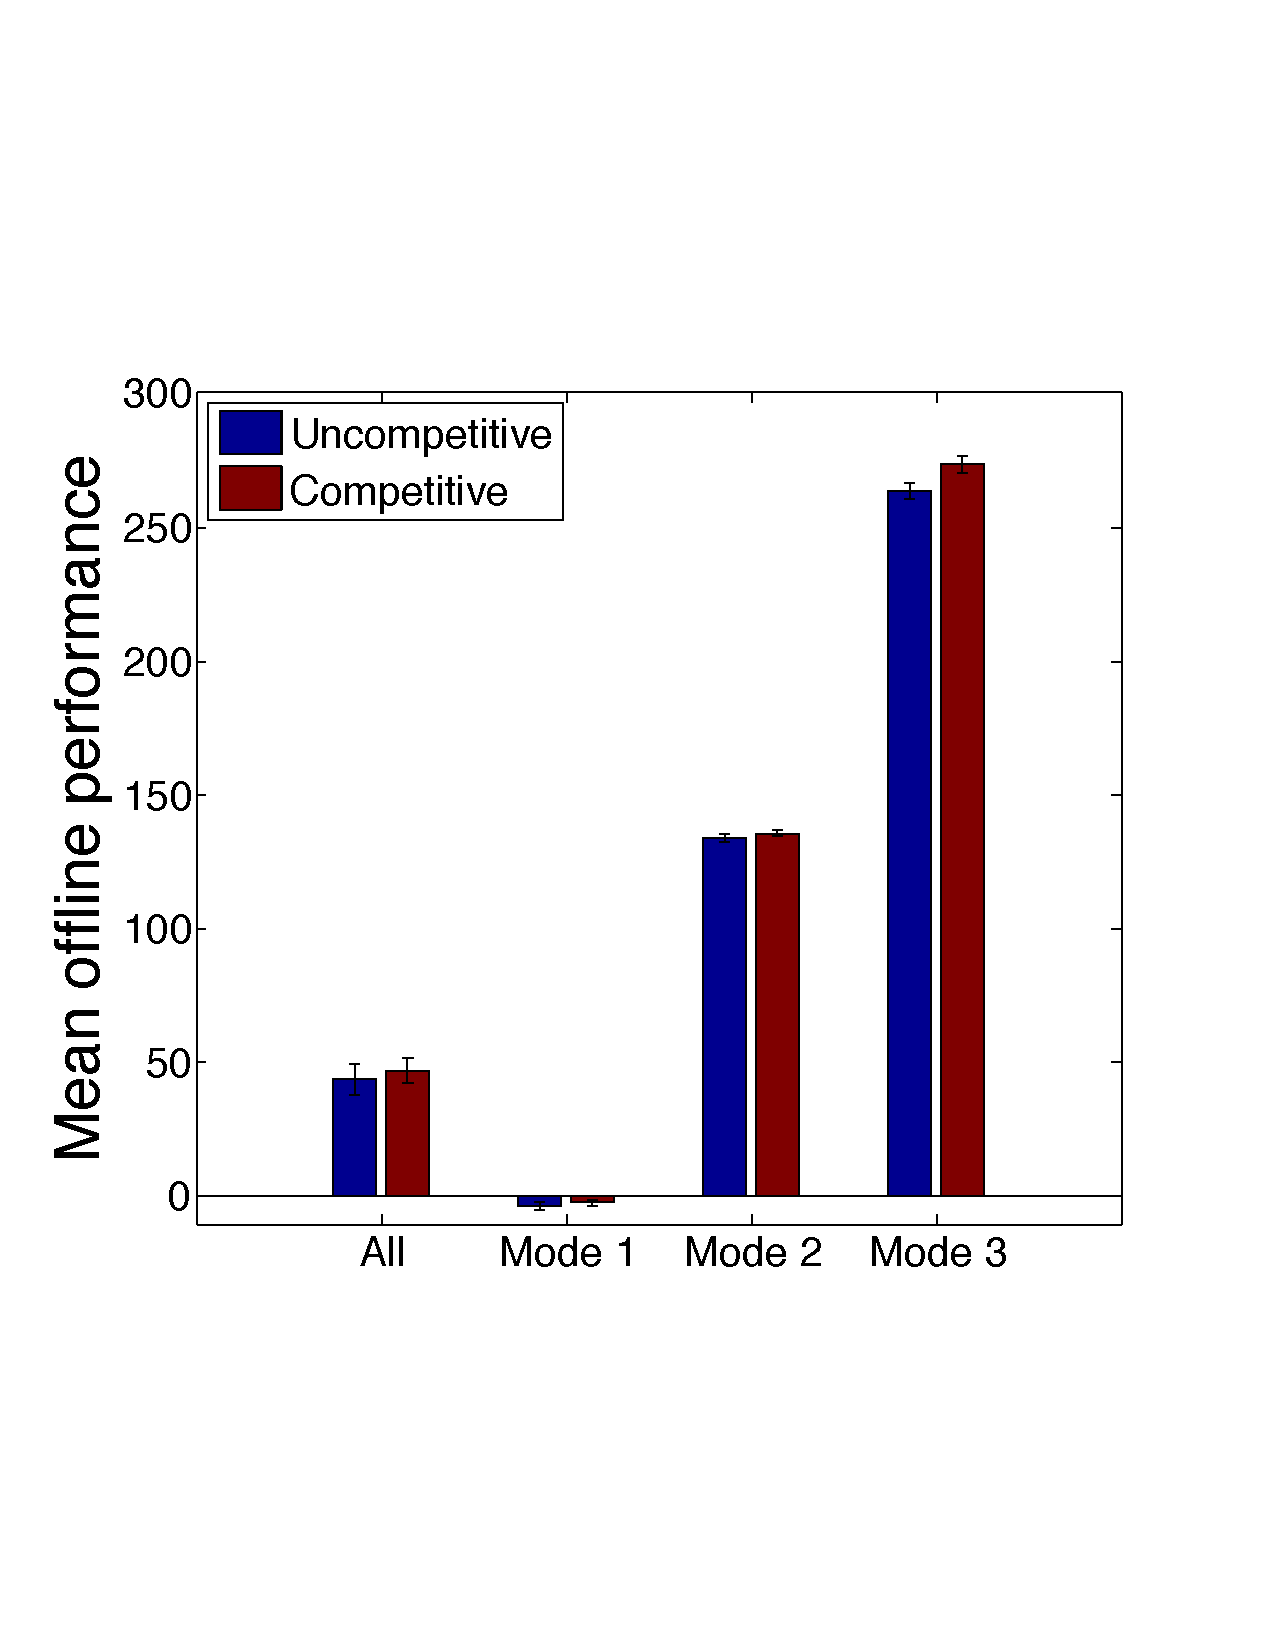
\includegraphics[width=0.58\columnwidth, height=1.56in, trim=0 0 0 0, clip]{CompetitionPerMode}&
%\includegraphics[width=0.38\columnwidth, height=1.56in, trim=0 0 0 0, clip]{FacialExpressionPerGender}&
%\includegraphics[width=0.50\columnwidth, height=1.56in, trim=0 0 0 0, clip]{CompetitionPerAge} \\
%(a)&(b)
%\end{tabular}
%%\vspace{-4mm}
%\caption{Mean final offline performance for agents %(a) across and in the three modes distributed in Figure \ref{HisFinalOfflinePerformance}, trained with and without competitiveness, 
%trained by (a) female and male subjects with and without facial expression, (b) trainers in three age groups with and without competitiveness. Note: black bars stand for standard error.}
%%\vspace{-5mm}
%\label{GengerAge}
%\end{figure}

%\paragraph{Role of Age}
%\subsection{Role of Age}
%\begin{figure}[tb]
%%\vspace{-2mm}
%%\hspace{4mm}
%\centering
%%\begin{tabular}{c c}
%\includegraphics[width=\columnwidth,trim=0 6 6 6, clip]{CompetitionPerAge}
%%\includegraphics[width=0.495\columnwidth,trim=0 0 0 0, clip]{MedianOfflinePerformance} \\
%%a&b
%%\end{tabular}
%%\vspace{-2mm}
%\caption{Mean final offline performance for agents in three age groups, with and without competitiveness. Note: black bars stand for standard error. }
%%\vspace{-8mm}
%\label{mode}
%\end{figure}

%\begin{table}
%%\renewcommand{\arraystretch}{1.5}
%%\captionsetup{font=footnotesize}
%\centering
%\begin{tabular}{ r | l | l | l }
%\toprule
%%\multirow{2}{*}{Condition} &Non-social  &  Social behavior \\
%& \textbf{Under 13} & \textbf{13 to 30}  & \textbf{Above 30}\\
%\toprule
%\textbf{Perfor. mode} & $p$ = $\textbf{0}^{\ast}$ & $p$ = $\textbf{0}^{\ast}$ &  $p$ = $\textbf{0}^{\ast}$ \\
%\hline
%\textbf{Competition} & $p$ = \textbf{0.0848} & $p = 0.6189$ & $p$ = $\textbf{0.033}^{\ast}$ \\
%\hline
%\textbf{Gender} & $p = 0.7827$ & $p$ = \textbf{0.0967} & $p = 0.6443$\\
%\hline
%\textbf{FE} & $p = 0.6634$ & $p = 0.9976$ & $p = 0.1225$ \\
%\toprule
%\end{tabular}
%\caption{ANOVA test of factor effect on final agent performance for trainers under 13 years old, 13 to 30 years old and older than 30 years old. $^{\ast}$Statistically significant.}
%%\vspace{-4mm}
%\label{age}
%\end{table}

%%Although Section \ref{sec:per} showed that overall, `age' has insignificant effect on agent's final offline performance, 
%We also suspected that `facial expression' and `competition' affect agent training by trainers within different agent groups differently, %the agent's competitive feedback and telling subjects to use facial expressions as a separate training channel have different effects on subjects of different ages, 
%since age differences largely account for reaction time differences \cite{deary2005reaction} and both brain size and cognitive ability increase until young adulthood and then decrease \cite{rushton1996brain}. %Moreover, our results show that `age' has some effect on agent final performance trained by female subjects ($F(1,185)$ = $2.61$, $p$ = $0.076$, $\eta_{p}^{2}$ = $0.027$). %\sw{This is vague.  How are they different and why? Support with citations}\HH{I would talk about 'cognitive' ability. Maybe you can find papers about sensemaking ability as a function of age.}. 
%
%To investigate the role of age, we did n-way ANOVA test with the other four factors on agent final performance for trainers within the three age groups separately.% as shown in Table \ref{age}.%divided the subjects into three age groups: under 13, between 13 and 30, and over 30 years old. Then we analyzed the final offline performance for the three age groups.
%
%\begin{figure*}[t]
%%\vspace{-2mm}
%%\hspace{4mm}
%\centering
%\begin{tabular}{c c c}
%\includegraphics[width=0.6\columnwidth,trim=0 6 10 10, clip]{FinalOfflinePerformanceForUnder13} &
%\includegraphics[width=0.6\columnwidth,trim=0 6 10 10, clip]{FinalOfflinePerformanceFor1330}&
%\includegraphics[width=0.6\columnwidth,trim=0 6 10 10, clip]{FinalOfflinePerformanceForOlder30}\\
%a&b&c
%\end{tabular}
%\vspace{-2mm}
%\caption{Final offline performance for subjects under 13 (a), between 13 and 30 (b) and older than 30 years old (c). (FE=Facial Expression.)}
%\vspace{-3mm}
%\label{FinalOfflinePerformanceAge}
%\end{figure*}

%%From Table \ref{age} we can see that, `performance mode' still has significant effects on final agent performance for trainers within the three age groups: under 13, 13 to 30 and older than 30 years old ($p = 0$). 
%%Moreover, for trainers under 13 years old, `facial expression' has no effect on final agent performance ($F[1,241] = 0.19, p = 0.6634, \eta_{p}^{2} = 0.0008$) and there is no difference between agent training by female and male subjects ($F[1,241] = 0.08, p = 0.7827, \eta_{p}^{2} = 0.0003$), but 
%Our results show that `age' has some effect on agent performance trained by female subjects with those between 13 to 30 years old training agents the worst ($F(1,185)$ = $2.61$, $p$ = $0.076$, $\eta_{p}^{2}$ = $0.027$).
%Moreover, Figure \ref{ModeGengerAge}c shows that `competition' can significantly motivate trainers older than 30 years old to train the agent better ($F(1,123)$ = $4.65$, $p$ = $0.03$, $\eta_{p}^{2}$ = $0.036$)  %not trainers younger than 30 years old. %under 13 years old ($F[1,241]$ = $2.99$, $p$ = $0.085$, $\eta_{p}^{2}$ = $0.012$), %($F[1,241] = 2.99, p = 0.0848, \eta_{p}^{2} = 0.0123$), 
%%though not significant. 
%but not %has no effect on trainers 
%those younger than 30 years old. Furthermore, for trainers between 13 to 30 years old, males trained better than females ($F(1,116)$ = $5.75$, $p$ = $0.02$, $\eta_{p}^{2}$ = $0.047$).
%%agents trained by male subjects performed better than those by female ones %`competition' have no effect on agent performance %$F[1,116] = 0, p = 0.9976, \eta_{p}^{2} = 0$ and 
%%($F(1,116)$ = $5.75$, $p$ = $0.02$, $\eta_{p}^{2}$ = $0.047$). %($F[1,116] = 0.25, p = 0.6189, \eta_{p}^{2} = 0.0021$), 
%%but agents trained by male subjects performed better than those by female ones %there is almost significant difference between agent performance trained by female and male subjects 
%%($F[1,116]$ = $2.8$, $p$ = $0.098$, $\eta_{p}^{2}$ = $0.024$). %($F[1,116] = 2.8, p = 0.0967, \eta_{p}^{2} = 0.0236$). 
%%For trainers older than 30 years old, %`facial expression' has some effect on final agent performance though not significant ($F[1,123] = 2.42, p = 0.1225, \eta_{p}^{2} = 0.0193$) %and there is no significant difference between agent performance trained by female and male subjects ($F[1,123] = 0.21, p = 0.6443, \eta_{p}^{2} = 0.0017$), but 
%%`competition' can significantly motivate trainers to train agent better ($F[1,123]$ = $4.65$, $p$ = $0.03$, $\eta_{p}^{2}$ = $0.036$). %($F[1,123] = 4.65, p = 0.033, \eta_{p}^{2} = 0.0364$). 
%While examining `facial expression', we found that it %has some negative effect on agent training by subjects older than 30 years old ($F(1,123)$ = $2.42$, $p$ = $0.12$, $\eta_{p}^{2}$ = $0.019$), %($F[1,123] = 2.42, p = 0.1225, \eta_{p}^{2} = 0.0193$), 
%%and %there is a two-way interaction between `facial expression' and `gender' for trainers younger than 13 years old: `facial expression' 
%ruins agent learning trained by female subjects younger than 13 years old ($F(1,232)$ = $7.1$, $p$ = $0.008$, $\eta_{p}^{2}$ = $0.03$).%but no effect by trainers under 30 years old. 

% In summary, our results suggest that %`facial expression' -- telling subjects to use facial expressions as a separate training channel has some effect on final agent performance trained by subjects older than 30 years old and
%  `competition' can significantly motivate subjects older than 30 years old to train agent better not those younger ones. %than 30 years old. 
% Moreover, %for trainers between 13 and 30 years old, agents trained by male subjects performed better than those by female ones and %the two-way interaction effect was on trainers younger than 13 years old.
% %telling to use facial expression as a separate training channel 
% `facial expression' has a negative effect on agent learning trained by female subjects younger than 13 years old. %, but has some negative effect on agent learning by subjects younger than 13 years old. %In addition, our results also show that there is almost significant difference between final agent performance trained by female and male subjects between 13 and 30 years old. 
%
%Since the brain size and cognitive ability show a curvilinear relation with age: increasing to young adulthood and then decreasing \cite{rushton1996brain}, 
%
%These results provide a deep insight on human training the agent especially when we allow agents to learn from facial expressions, though not significant. 

%\vspace{1mm}
%\section{Discussion}
%\label{sec:dis}
%
%The results of our experiment shed a lot of light on the way subjects interact with learning agents via TAMER and support prior studies (Li et al. 2014a) demonstrating the importance of bi-directional interaction and competitive elements in the training interface. %Specifically, our results show that `competition' can significantly improve agent learning especially trained by those who can train agents to perform better. 
%%When examining the gender, our results demonstrate that `facial expression'---telling subjects to use facial expressions as a separate training channel has a significantly negative effect on agent training by females subjects, and `competition' can significantly improve agent learning trained by male subjects.  Furthermore, `competition' can significantly motivate subjects older than 30 years old to train agent better, but has some negative effect on agent learning trained by subjects younger than 13 years old. 
%However, though the results are significant, some differences between the mean performances are not big. We believe that it could be because of the game score mechanism. For example, when motivated by `competition', trainers may have encouraged behaviors such as collecting mushrooms and killing a monster, which are much more difficult than collecting coins. However, the scoring metric rewards the agent equally when it kills monsters, collects coins, and no score for collecting mushrooms. The trainers may have put more emphasis on these difficult behaviors without a large increase in score, especially those subjects who can train agents to be in the second and third modes in Figure \ref{HisFinalOfflinePerformance}. 


%while a good strategy for getting a high score is to singlemindedly move to the right as fast as possible and reach the finishing line. %, even though the two are rewarded equally by the scoring metric.   Trainers may also have trained the agent to play the way they themselves play, e.g., walking back and forth to collect mushrooms or coins or smash blocks, while a good strategy for getting a high score is to singlemindedly move to the right as fast as possible and reach the finishing line.%However, a key limitation of our results is that, despite the large number of subjects, they are not statistically significant. One possible reason is that trainers, due to their prior familiarity with the domain, may have tried to teach the agent behavior that they consider good but which is not rewarded by the scoring metric from the Reinforcement Learning Competition that we employed.  For example, the scoring metric only rewards the agent when it kills monsters, collects coins, and reaches the finishing line but trainers may have also encouraged other behaviors such as collecting mushrooms.  Similarly, since killing a monster is much more difficult than collecting coins, the trainers may have put more emphasis on the former, even though the two are rewarded equally by the scoring metric.   Trainers may also have trained the agent to play the way they themselves play, e.g., walking back and forth to collect mushrooms or coins or smash blocks, while a good strategy for getting a high score is to singlemindedly move to the right as fast as possible and reach the finishing line.  A similar effect was observed by Li et al.\ \cite{li2014leveraging,li2014learning}, in which subjects training TAMER agents to play Tetris seemed to encourage clearing multiple lines at a time, though this yielded no additional rewards in the scoring metric they employed.  Teaching such complex behaviors in such a short time is difficult and, if it is not rewarded by the scoring metric, may result in the poor performance seen in the first modes in the histograms in Figure \ref{HisFinalOfflinePerformance}. Further analysis is needed to get a deeper understanding of these results, e.g., analyzing the agent's learned behavior and the contribution of each element for the performance, evaluating performance with other scoring metrics, etc.


%Interestingly, similar gender differences were also observed by other researchers \cite{brody1993understanding}, where females express a wider variety of emotions than do males, both verbally and through facial expressions. This could relate to our results about the significant effect of `facial expression' on agent performance trained by female subjects, though more investigation needs to be made into whether females made more facial expressions than males in our experimental setting.
%%In addition, more analysis of the video data is needed to
%%understand the reason for the negative effect caused by %telling subjects to use facial expressions as a separate training channel, 
%%`facial expression', e.g., to determine whether the negative effect on
%%female subjects is due to females making more pronounced facial
%%expressions. 
%However, these results point the way to further
%analysis of the correlation between key press feedback and
%facial expressions by considering gender and age differences.
%%opening the door to TAMER systems that can learn only from facial expressions. 
%%It also underscores the fact that, if we
%%want the agent to learn from facial expressions and we tell
%%trainers that they can use facial expressions to train the
%%agent, then we need to find a way to balance these negative
%%effects. Otherwise, it may be better not to let them know that
%%the agent can learn from facial expressions at all.


%\vspace{-4mm}

%\paragraph{Analysis of Facial Feedback}
\subsection{Analysis of Facial Feedback}

It is well known that facial expressions reflect inner feelings
and emotions. We assessed the informativeness of facial
expressions as a feedback signal. To this end, 3-D locations of 512
densely defined facial landmarks (see
Figure~\ref{landmarks}) were automatically detected and
tracked using the state-of-the-art method proposed by Jeni et
al.\ \cite{jeni2015dense}. Videos with a downsampled frame
rate of 20 fps were used in tracking. Data from 31 participants (5.5\% of the data analyzed) %\HH{(X\% of the data analysed)} 
were discarded due to methodological problems such as face
occlusion, talking, and chewing gum during the experiment. %\HH{state in numbers how many subjects were removed from the analysis here}. 
In
total 9,356,103 frames were tracked.  %\HH{should we say here how many hours on what types of high powered machines?}. %(110 subjects for the control condition, 101 subjects for the facial expression
%condition, 158 subjects for the competitive condition, 161
%subjects for competitive facial expression condition).
To eliminate rigid head movements, the tracked faces were
shape-normalized by removing translation, rotation and scale.
Since the normalized faces are approximately frontal with
respect to the camera, we ignored the depth ($z$) coordinates
of the normalized landmarks. Consequently, 1024 location
parameters were obtained per frame. %(512 landmarks $\times$ $x$, $y$ coordinates)
%cond1: 110, 1,917,557, m=1.7432e+04, s=3.1129e+03
%cond2: 101, 1,737,242, m=1.7200e+04, s=3.4708e+03
%cond3: 158, 2,876,593, m=1.8206e+04, s=2.4188e+03
%cond4: 161, 2,824,711, m=1.7545e+04, s=2.8530e+03

\begin{figure}[htb]
\centering

\includegraphics[height=0.56\columnwidth]{markers2.pdf}
\caption{512 tracked facial landmarks.}
\label{landmarks}
\end{figure}

\subsubsection{Facial Expressiveness}

To analyze facial activity levels of different conditions, we
computed the standard deviation of the landmark positions within a 2$s$
interval around each key press feedback (1$s$ before to 1$s$
after). The 2$s$ interval is chosen because the great majority of facial expressions of felt emotions last between 0.5 second and 4 seconds \cite{ekman1984expression} and the differences of standard deviations between conditions are largest in this case. Standard deviations were averaged for each
subject in each condition. Then, we analyzed the significant
differences in vertical ($y$) and horizontal ($x$) facial
movements, between different conditions using a t-test. The computed
$p$ values for $x$ and $y$ coordinates were combined as
$p_c=\sqrt{{p_x}^2+{p_y}^2}$ to represent the significance level
for each landmark position as one parameter.



\begin{figure*}[t!]
\begin{center}%\HH{could perhaps get away with making this table half a column and have the faces in two rows ... it feels like it's quite big or even just 4 in a row and remove (a)... do we really need (a)?}

\begin{tabular}{c c c c c}
 % 
\includegraphics[height=0.4\columnwidth]{markers2.pdf} &
 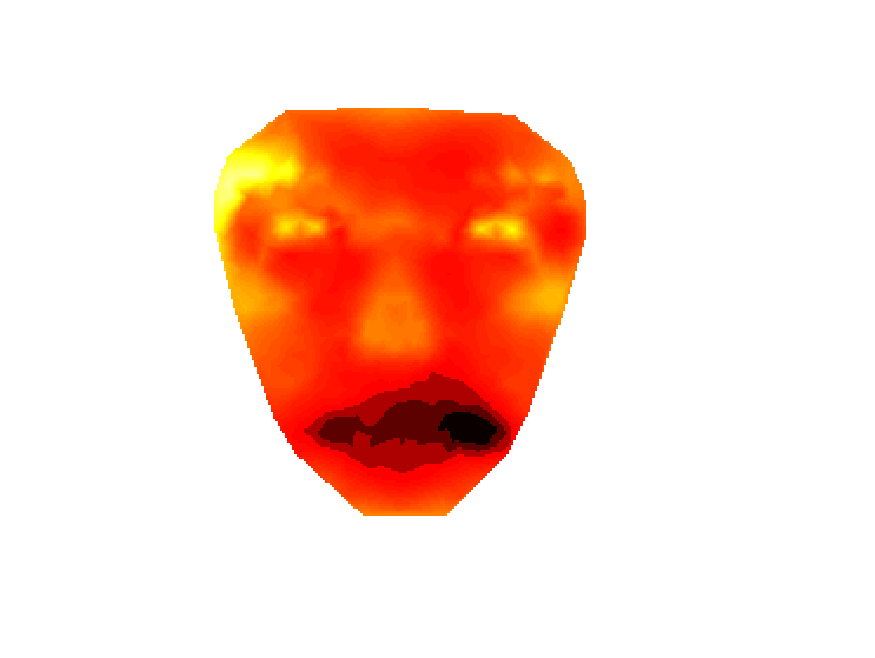
\includegraphics[height=0.5\columnwidth]{fc1-2.pdf}&
  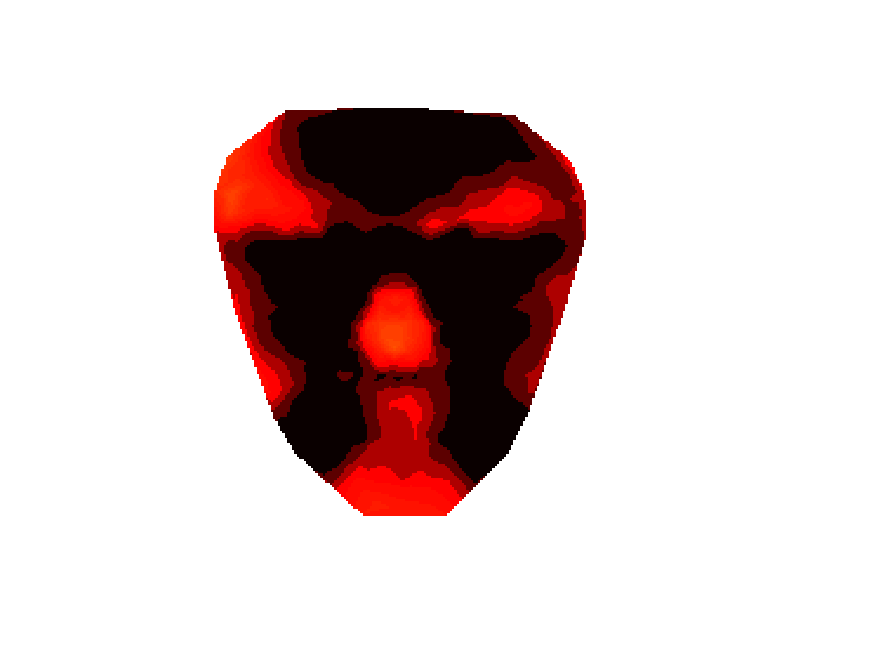
\includegraphics[height=0.5\columnwidth]{fc3-4.pdf}   &\includegraphics[height=0.5\columnwidth]{fc1-3.pdf}&
  \includegraphics[height=0.5\columnwidth]{fc2-4.pdf}   &\includegraphics[height=0.5\columnwidth]{fc_legend.pdf}  \\
    (a)& (b)& (c)& (d)\\%& (e)\\
 \end{tabular}
\end{center}
%\vspace{-4mm} 
\caption{%(a) 512 tracked facial landmarks.
Significance level ($p_c$) of differences in expressiveness
between different conditions: (a) \emph{control vs. facial
expression}, (b) \emph{competitive vs. competitive facial
expression}, (c) \emph{control vs. competitive}, and (d)
\emph{facial expression vs. competitive facial expression}.
Dark gray or black colored ($p_c<0.05$) regions display
significantly different activeness between the corresponding
conditions.} \label{markers}
%\vspace{-4mm}
\end{figure*}

Figures~\ref{markers}(a--d) visualize the significance level of
differences ($p_c$) in expressiveness between different
conditions. The visualized $p_c$ values for transition
locations between detected landmarks were computed by linear
interpolation. When we analyze the significant differences
($p_c<0.05$) in facial activeness between different conditions,
it is seen that the mouth region is more dynamic in the \emph{facial
expression condition} compared to the \emph{control condition}
(Figure~\ref{markers}(a)). Similarly, the deviation of movements in the 
mouth, upper cheek, and forehead regions for the \emph{competitive
facial expression condition} are higher than those of the
\emph{competitive condition} (Figure~\ref{markers}(b)). These
results can be explained by the fact that subjects exaggerate
their expressions in facial expression conditions. In
competitive conditions, almost the whole surface of the face has
higher activity levels in comparison to the control conditions as
shown in Figure~\ref{markers}(c--d). These findings suggest
that competitive conditions can elevate facial expressiveness. 

In summary, consistent with our hypotheses, both agent's competitive feedback and telling trainers to use facial expressions as additional channel to train agents could increase the trainer's facial expressiveness. In addition, the largest difference was observed in Figure~\ref{markers}(c) between the control and competitive conditions, which indicates that the effect of the competitive situation on expressiveness could be larger than that effect of the facial expression condition. %Moreover, 
%some facial expressions seems to exaggerate eyebrow only regions compared to the baseline. Could this indicate that there is more negative feedback (frowning being observed).
%ask jeff
%\HH{do we have space to discuss the fact that some facial expressions seems to exaggerate eyebrow only regions compared to the baseline. Could this indicate that there is more negative feedback (frowning being observed?)}

\subsubsection{Classification of Positive and Negative Feedback with Facial Expressions}
\label{sec:classify}

\begin{table}[t!]
%\vspace{-2mm}
%\vspace{2mm}
\begin{center}
\resizebox{1\columnwidth}{!}{ \footnotesize
\renewcommand\arraystretch{1.1}
\begin{tabular}{clccc}
\toprule[.8pt]
                                &Condition&Positive	&Negative	&Total\\
\midrule[.8pt]
\multirow{3}{*}{\rotatebox{90}{{\parbox{1.35cm}{\footnotesize{Proposed Method}}}}} &&&&\\ [-2.5ex]
&Control                        &0.47    &0.68    &0.57	\\
&Facial Expression              &0.49    &0.69    &0.59 	\\
&Competitive                    &0.61    &0.59    &0.60  \\
&Competitive Facial Expression  &0.72    &0.59    &0.67  \\
\midrule[.8pt]
\multirow{4}{*}{\rotatebox{90}{{\parbox{1.2cm}{\footnotesize{Random Baseline}}}}} &&&&\\ [-2.5ex]
&Control                        &0.50	    &0.50	    &0.50 \\
&Facial Expression              &0.42	    &0.58	    &0.51 \\
&Competitive                    &0.52 		&0.48		&0.50 \\
&Competitive Facial Expression  &0.58 		&0.42 		&0.51 \\
\bottomrule[.8pt]
\end{tabular}
}\vspace{.4cm}
\caption{\label{table:feedAcc} Accuracy of classifying positive
and negative feedback using facial responses.} %\vspace{.4cm}
\end{center}
%\vspace{-6mm}
\end{table}

Next, we investigated the discriminative power of facial
responses for classifying positive and negative feedback. To
obtain a compact representation for facial movement parameters,
Principal Component Analysis (PCA) was used to reduce 1024
coordinate values to 20 principle components while retaining
$99.6\%$ of the variance. The mean, median, standard deviation,
maximum, minimum values of each principle component for 2$s$
intervals around each positive and negative feedback key press
(1$s$ before to 1$s$ after) were computed. These statistics can fairly describe the temporal movement characteristics of expressions within that interval \cite{cohn2009detecting,dibeklioglu2015recognition,dibekliouglu2015multimodal}. By
concatenating these features, 100-dimensional feature vectors were
obtained. Using a t-test, features that do not significantly
differ ($p>0.001$) between positive and negative feedback were
% identified, and 
removed. Random forest classifiers \cite{breiman2001random} %\SW{cite} 
using 300 trees were then trained using the resulting features.
 %(n predictors for splitting at each node).
Class labels for random baseline are assigned by drawing a random class label according to the ratio of positive and negative class labels from the training set.
%The random baseline is calculated based on the probabilities of 
%the positive and negative class. 

Our experimental scenario learns facial patterns of the
users in the first five minutes of the game, and classifies their
positive and negative feedback during the rest of the game. A five-fold cross-validation scheme was used. While
feedback in the first five minutes from fold $i$, and all
feedback from the remaining folds were used for feature
selection and training, unseen feedback from fold $i$ were
used for experimental evaluation (around 10 minutes). There was no subject overlap between
folds. %\textcolor[rgb]{1.00,0.00,0.00}{
85,429 positive and 79,585
negative feedback instances were used in the experiment.
%} 
As shown in
Table~\ref{table:feedAcc}, the use of facial expressions
significantly ($p<0.001$) outperformed the random baseline in each
condition except for classifying positive feedback in the 
\emph{control} condition. The highest accuracy was achieved for the
\emph{competitive facial expression} condition, followed by the
\emph{competitive} condition. This can be explained by the
increased facial expressivity due to the competitive setting and posed facial expressions.  As
expected, the proposed method provided higher accuracies for
facial expression conditions.
% to
% \emph{control} and \emph{competitive} conditions.


Overall, our study takes a first step towards enabling agents to learn from facial expressions by investigating correlations between facial expressions and key-press feedback.  Obviously, a critical future step would be to use classifiers trained in this way to actually train agents, thus reducing the need for explicit key-press feedback.  

%Unfortunately, such a step is well beyond the scope of this paper since it cannot be accomplished using the data gathered for our study. This is because learning via TAMER, as in any reinforcement-learning setting, is an interactive process, in which the learner's behavior affects what states are visited and thus what data is gathered.  Since all our data was gathered by agents learning only from key-press feedback, training agents using facial-expression feedback on this same data would not be meaningful: if performance declined, there would be no way to determine whether the cause was a change in the form of feedback or a discrepancy between the states visited by the recorded data and those visited by the learned policy.  
%
%Consequently, training agents using facial-expression feedback will require conducting a new study with new subjects, an important avenue for future work.

\begin{figure*}[htb]
%\vspace{-2mm}
%\hspace{4mm}
\centering
\begin{tabular}{c c c c}
\includegraphics[width=0.95\columnwidth]{cond1.pdf}&
\includegraphics[width=0.95\columnwidth]{cond2.pdf}\\
(a) Control condition & (b) Facial Expression condition\\
\includegraphics[width=0.95\columnwidth]{cond3.pdf}&
\includegraphics[width=0.95\columnwidth]{cond4.pdf}\\
(c) Competitive condition & (d) Competitive Facial Expression condition
%\vspace{-3mm}
\end{tabular}
\caption{Offline performance of agent learning from predicted feedback with facial expressions, compared to learning from keypress feedback and random feedback for all four conditions. }%(a) control condition, (b) facial expression condition, (c) competitive condition and (d) competitive facial expression condition.}%: a) Control condition, b) FE condition, c) Competitive condition and d) Competitive FE condition (FE=Facial Expression). %\HH{Could it make sense to actually color the bars here according to the highlest level that was reached for a given bar? It might help in better expalaining the multi-level scoring}}
%\vspace{-6mm}
\label{learning_from_predicted}
\end{figure*}

\subsection{Learning from Facial Feedback}

Then, to examine whether an agent can learn from the human trainer's facial expressions, we use the above trained model to predict human reward with human trainer's facial expressions at the time when keypress feedback was given. Ideally, we would run a new experiment where the trainer gives new facial expressions while watching the agent learn and use the predictor to get reward that we trained with. But that's prohibitively expensive so we need to do an evaluation with the data we have, and the closest approximation is to not use the early data to train the predictor but save it for implicit learning once we have trained the predictor on later data, or vice versa. 

Therefore, to get predicted human reward for the complete training trajectory for each participant, we first trained the model with the same above process in Section \ref{sec:classify}, to predict the unseen feedback after the first five minutes' training. For predicting feedback during the first five minutes, the training process is the same, except that the model training was done with data after the first five minutes' training. Then we use the predicted feedback to train agents with recorded data, record the learning policy per 200 time steps, and test the offline performance of the learning policy for 20 games each. The whole process was repeated for three trials for both learning from predicted feedback and random feedback. The performance for each condition is averaged over the three trials. %\sw{I think you need to much more clearly motivate why you are doing the evaluation in this way.  You need to say that, ideally, you'd run a new experiment where the trainer gave new facial expressions while watching the agent learn and you used your predictor to get reward that you trained with.  But that's prohibitively expensive so you need to do an evaluation with the data you have, and the closest approximation is to not use the early data to train the predictor but save it for implicit learning once you've trained the predictor on later data.}

We compare the agent's learning performance with predicted feedback to random feedback and keypress feedback, as shown in Figure \ref{learning_from_predicted}. From Figure \ref{learning_from_predicted} we can see that agent learning from facial expressions performs better than from random feedback, though still worse than learning from explicit feedback. Even though the learning from facial expressions is modest, the fact that the agent is able to learn at all given only implicit feedback is an exciting success and opens up a lot of new potentials for learning from human reward that should be explored. We believe in future work, an improved model with higher prediction accuracy would allow the agent to learn better from facial expressions.


%both competition and telling to use facial expressions can elevate the human trainer's facial expressiveness and result in higher accuracy of predicting positive and negative feedback using facial responses, 
%taking the first step for exploring methods of facilitating agents to learn from facial expressions in future work.

%When considering gender, our results suggest that telling female subjects to use facial expressions as a separate training channel has a negative effect on training agents but not for male subjects. However, the agent's competitive feedback can improve the agent's learning only when female subjects were told to use facial expressions as a separate training channel and when male subjects were not told to. 

%When considering age group, our results suggest that the agent's competitive feedback and telling subjects to use facial expressions as a separate training channel have different effects on different age groups. Specifically, telling subjects to use facial expression as a separate training channel has little or even no effect on the agent's learning for subjects less 30 years old, but has a negative effect on the agent's learning for subjects more than 30 years old. In addition, the agent's competitive feedback can improve the agent's learning when trained by subjects more than 30 years old, has no clear effect on subjects less than 13 years old, and improves the agent's learning for subjects between 13 and 30 years old only when they are told to use facial expressions as a separate training channel. %Finally, these findings provide a deep insight into how to use facial expression as reward signal to train the agent.

%From these analysis we can see that, generally speaking, knowing facial expression as training signal has negative effect on agent training, competitiveness can increase agent performance and competitiveness can compensate this negative effect. In term of different age groups, this phenomenon can be found especially on subjects older than 31 years old. But for subjects younger than 30 years old it does not work well or it may work person-specificly or gender-specific.
%
%In term of gender difference, generally speaking, knowing facial expression as training signal has negative effect on agent training happens on female subjects but unclear for male subjects. However, after looking into the gender difference within different age groups, we found that this negative effect happens on female subjects younger than 30 years old but on male subjects older than 30 years old.
%
%On average, competitiveness only works on female subjects when they were told to use facial expression as training signal, but unclear for male subjects. After looking into the gender difference within different age groups, for female subjects, competitiveness works whenever they were told to use facial expression as training signal for those older than 31 years old, but for those younger than 12 years old, it only works when they were told to use facial expression as training signal. This phenomenon remains unclear for female subjects between 13 and 30 years old.
%
%For male subjects, for for those younger than 12 years old, competitiveness works they were not told to use facial expression as training signal, but for those older than 13 years old, it only works when they were told to use facial expression as training signal.

%Future work will focus on further investigating the role of facial expressions in agent learning from human reward and its effects as a function of age and gender. This will enable us to explore the potential of allowing the agent to learn from it. 
%%\HH{I removed this part - we don't want to give away too many of our ideas!} First, we aim to investigate whether there is a correlation between facial expressions and explicit human reward. Second, we aim to use machine learning to train functions that predict explicit reward given implicit reward, so that implicit reward can be directly used within TAMER even when explicit feedback is not available.  
%Finally, we aim to find a way to balance the negative effects caused by telling trainers to use facial expressions as a reward signal, so as to maximize its potential as a learning signal.

\vspace{2mm}

\section{Discussion and Open Questions}
\label{sec:doq}

Our experiments highlight clearly that the relationship between the reward signal and the nature of facial expressions and how human trainers chose to use them still needs to be explored further. Our further results with recorded data indicate that an agent can learn from facial expressions via interpreting as reward signals, though the learning is modest.
%Training agents using facial-expression feedback will require conducting a new study with new subjects. However, our results with recorded data indicate that an agent can learn from facial expressions via interpreting as reward signals, though the learning is modest.
%Unfortunately, such a step is well beyond the scope of this paper since it cannot be accomplished using the data gathered for our study. This is because learning via TAMER, as in any reinforcement-learning setting, is an interactive process, in which the learner's behavior affects what states are visited and thus what data is gathered.  %Since all our data was gathered by agents learning only from key-press feedback, training agents using facial-expression feedback on this same data would not be meaningful: if performance declined, there would be no way to determine whether the cause was a change in the form of feedback or a discrepancy between the states visited by the recorded data and those visited by the learned policy.  
%Consequently, training agents using facial-expression feedback will require conducting a new study with new subjects, an important avenue for future work. 
However, before we begin to learn feedback signals from facial expressions in fairly unconstrained settings, we highlight a few future challenges:

\subsection{Efficiency of using face and keypress input}
Our experiments highlight significant differences between the performance of agents when subjects were told facial expressions would be used and when they were not. Importantly, despite differences in the quality of key-press feedback in the facial expression conditions, the number of feedback instances was the same. This suggests a negative effect related to the cognitive load of being told to make facial expressions. To measure the effects of cognitive load fully in this setting remains an open challenge since we do not know fully what the facial expressions mean when they are more spontaneous. This is evidenced by the results in Table \ref{table:feedAcc}, where the reward signal of the facial expressions in the control condition were the most difficult to predict. 

\subsection{Feedback quality in relation to temporal factor}
As shown in Figure \ref{feedback}, the amount of feedback reduces over time in general. Does keypress feedback quality reduce as a result? Does facial feedback correspond to feedback better quality as time increases? Further investigation is neccessary to understand whether the nature of the feedback in terms of reaction time, length of expression (the time it takes to go from neutral to the expression and back to neutral), intensity of the facial expression, amongst others.


\subsection{Linking facial behaviour to positive and negative reward}
We see that predicting facial expressions in more competitive scenarios is generally easier, particularly if the subjects are told that posed expressions correspond to positive and negative reward. However, we do not know how spontaneous as opposed to posed facial expressions might contribute to agent learning. It could also be that these require the learning of different models, even within the same condition. We also need to understand whether facial expression feedback might also be useful for agent learning even when no key press feedback is given. 

\vspace{2mm}

\section{Conclusion}% \& Future Work} 
\label{sec:con}
%\HH{I have not edited this. I'd like to wait till the Results section is a bit more finalised.}
This paper investigated the effect of an agent's competitive feedback and the potential for agents to learn from human trainers' facial expressions.
%telling trainers to use facial expressions as a separate training channel on agent's learning. %in different genders and ages. 
To this end, we conducted the first large-scale study with usable data from 498 participants (children and adults) by implementing TAMER in the Infinite Mario domain.  Our results show for the first time that a TAMER agent can successfully learn to play Infinite Mario, generalizing prior work in other game environments.  In addition, our experiment supports previous studies demonstrating the importance of bi-directional feedback and competitive elements in the training interface and shows the negative effect of telling female trainers to use facial expressions for training. %Specifically, `competition' can significantly improve agent learning especially trained by subjects who trained agents best %, male subjects 
%and subjects older than 30 years old. %. When considering gender, `competition' can significantly improve agent learning trained by male subjects. When considering age, `competition' can significantly motivate subjects older than 30 years old to train agent better. 
Furthermore, %`facial expression'---
%telling to use facial expressions as a separate training channel has a significantly negative effect on agent training by female subjects, %especially those who are younger than 13 years old and train agents insufficiently well, 
our analysis shows that telling trainers to use facial expressions makes them inclined to exaggerate their expressions, resulting in higher accuracy for predicting positive and negative feedback using facial expressions. Competitive conditions also elevated facial expressiveness and further increased predicted accuracy. This has significant consequences for the design of agent learning systems that wish to take into account a trainer's spontaneous facial expressions as a reward signal. Finally, our results indicate that an agent can learn from facial expressions via interpreting as reward signals, though the learning is modest. Further investigation into the nature of spontaneous and posed facial expressions is needed, in particular in terms of their relation to feedback quality and quantity.

%\section{Conclusion}
%The conclusion goes here.





% if have a single appendix:
%\appendix[Proof of the Zonklar Equations]
% or
%\appendix  % for no appendix heading
% do not use \section anymore after \appendix, only \section*
% is possibly needed

% use appendices with more than one appendix
% then use \section to start each appendix
% you must declare a \section before using any
% \subsection or using \label (\appendices by itself
% starts a section numbered zero.)
%


%\appendices
%\section{Proof of the First Zonklar Equation}
%Appendix one text goes here.
%
%% you can choose not to have a title for an appendix
%% if you want by leaving the argument blank
%\section{}
%Appendix two text goes here.
%
%
%% use section* for acknowledgment
%\ifCLASSOPTIONcompsoc
%  % The Computer Society usually uses the plural form
%  \section*{Acknowledgments}
%\else
%  % regular IEEE prefers the singular form
%  \section*{Acknowledgment}
%\fi
%
%
%The authors would like to thank...


% Can use something like this to put references on a page
% by themselves when using endfloat and the captionsoff option.
\ifCLASSOPTIONcaptionsoff
  \newpage
\fi



% trigger a \newpage just before the given reference
% number - used to balance the columns on the last page
% adjust value as needed - may need to be readjusted if
% the document is modified later
%\IEEEtriggeratref{8}
% The "triggered" command can be changed if desired:
%\IEEEtriggercmd{\enlargethispage{-5in}}

% references section

% can use a bibliography generated by BibTeX as a .bbl file
% BibTeX documentation can be easily obtained at:
% http://mirror.ctan.org/biblio/bibtex/contrib/doc/
% The IEEEtran BibTeX style support page is at:
% http://www.michaelshell.org/tex/ieeetran/bibtex/
%\bibliographystyle{IEEEtran}
% argument is your BibTeX string definitions and bibliography database(s)
%\bibliography{IEEEabrv,../bib/paper}

\bibliographystyle{abbrv}
\bibliography{sigproc} 
%
% <OR> manually copy in the resultant .bbl file
% set second argument of \begin to the number of references
% (used to reserve space for the reference number labels box)
%\begin{thebibliography}{1}
%
%\bibitem{IEEEhowto:kopka}
%H.~Kopka and P.~W. Daly, \emph{A Guide to \LaTeX}, 3rd~ed.\hskip 1em plus
%  0.5em minus 0.4em\relax Harlow, England: Addison-Wesley, 1999.
%
%\end{thebibliography}

% biography section
% 
% If you have an EPS/PDF photo (graphicx package needed) extra braces are
% needed around the contents of the optional argument to biography to prevent
% the LaTeX parser from getting confused when it sees the complicated
% \includegraphics command within an optional argument. (You could create
% your own custom macro containing the \includegraphics command to make things
% simpler here.)
%\begin{IEEEbiography}[{\includegraphics[width=1in,height=1.25in,clip,keepaspectratio]{mshell}}]{Michael Shell}
% or if you just want to reserve a space for a photo:

\begin{IEEEbiography}{Guangliang Li}
Biography text here.
\end{IEEEbiography}

\begin{IEEEbiography}{Hamdi Dibeklio{\u{g}}lu}
Biography text here.
\end{IEEEbiography}

\begin{IEEEbiography}{Shimon Whiteson}
Biography text here.
\end{IEEEbiography}

\begin{IEEEbiography}{Hayley Hung}
Biography text here.
\end{IEEEbiography}

% if you will not have a photo at all:
%\begin{IEEEbiographynophoto}{John Doe}
%Biography text here.
%\end{IEEEbiographynophoto}

% insert where needed to balance the two columns on the last page with
% biographies
%\newpage

%\begin{IEEEbiographynophoto}{Jane Doe}
%Biography text here.
%\end{IEEEbiographynophoto}

% You can push biographies down or up by placing
% a \vfill before or after them. The appropriate
% use of \vfill depends on what kind of text is
% on the last page and whether or not the columns
% are being equalized.

%\vfill

% Can be used to pull up biographies so that the bottom of the last one
% is flush with the other column.
%\enlargethispage{-5in}



% that's all folks
\end{document}


